%
% Draft  document crimp.tex
% Notes on crimp formation in wool staples
%
 
\documentclass[titlepage,10pt]{article}  % Latex2e
\usepackage{graphicx,lscape,subfigure}
\usepackage{caption,rotating}
\usepackage{bm}
\usepackage{textcomp}
 

\title{ Staple crimp formation in the fleece of Merino sheep}
\author{Neville Jackson and Jim Watts }
\date{22 Dec 2016} 

 
\begin{document} 
 
\maketitle      
\tableofcontents

\clearpage
\section{Acknowledgement}
Some of the ideas developed here originally arose in discussions of one of the authors with Dr Paul Swan when we worked together at CSIRO Division of Wool Technology. We would like to acknowledge Paul's contribution and point to his PhD Thesis~\cite{swan:93} as a major work on crimp and fibre curvature in Australian Merino wool.


\clearpage
\section{Introduction} 
When it was discovered that wool fibres have ortho and para cortex (Horio and Kondo(1953)~\cite{hori:53}, and that these differed in amount of keratinization , resulting in a curved fibre , there was a temptation to conclude that this 'intrinsic fibre curvature' was {\em the} fibre property of importance, and that all other issues related to wool crimp, such as the 'crimp-set' acquired in a staple, were irrelevant. In the textile world this is probably correct.

In the sheep world, people continue to look at crimped wool staples, to wonder at the variety therein, and to make inferences from what they see to what they think about wool quality. There are problems with this. Wool  quality is poorly defined, how staples get to look the way they do is not fully understood, and the relationship betwen the two is mostly a matter of guesswork.

What we want to try to do here is clarify some issues about the way crimp forms in wool staples and the extent to which crimp and staple appearance relate to basic fibre properties.

\clearpage
\section{A three-dimensional physical model for staple crimp formation}
There have been a number of theories of staple crimp  formation invoking movement of follicles in the skin (Chapman(1965)~\cite{chap:65} or movement of the fibre shaft within the follicle (Nagorcka(1981)~\cite{nago:81}.  We reject any theory invoking movement within the skin or follicle on the grounds that it is unnecessary. Crimp formation can be explained as a simple 3-dimesional phenomenon. No biological harmonic movement is required. All that is required is continuous growth of  fibres with constant curvature.

A single wool fibre grows with near-constant curvature and if conditions are reasonable with a regular even growth rate. If there were no other fibres growing around it, it would simply curl around on itself and lie coiled up like a hose on the ground. Technically it would be a helix. 

Fibres do not grow singly. They are surrounded by a dense 'forest' of other fibres, all growing with approximately the same growth rate and intrinsic curvature. There is not sufficient space for each fibre to form an independent helix. There are lateral forces at fibre contact points, and there are longitudinal forces ( along the helix) caused by some fibres growing faster than  others. The lateral forces hold fibres into bundles, so the hypothetical single fibre helix becomes a bundle of fibres coiled together. The longitudinal forces stretch the helix bundles - like a stretched spring. The fibres are {\em set} into that stretched position by the conditions of heat and moisture in the fleece near the skin. There is no requirement for a continuous longitudinal force to hold the fibres in the stretched helix position. 

In a typical Merino wool the 'spring' is over-stretched into a dished sine wave, which is the form of crimp seen in most strains of Merino sheep.


\subsection{Single fibre model}
Let us see how this works in a 3D model. First one fibre. We start with a helix. Figure~\ref{fig:1}  shows a length of electrical copper wire coiled up into a helix (like a phone cord). 

%\documentclass{article}
%\usepackage{graphicx,subfigure}
%\begin{document}

\begin{figure}[!h]
  \centering
  \includegraphics[width=1.1\textwidth]{fig1.jpg}
%  P7060005.JPG is original
  \caption{A length of electrical copper wire coiled up into a helix}
  \label{fig:1}
\end{figure}

%\end{document}



Notice that the yellow coloured stripe is always on the outer side of the curved wire. This emulates the orthocortex which is always on the outer side of a curved fibre.

Now apply a longitudinal force and stretch the helix. The result is shown in Figure~\ref{fig:2} .

%\documentclass{article}
%\usepackage{graphicx,subfigure}
%\begin{document}

\begin{figure}[!h]
  \centering
   \includegraphics[width=0.9\textwidth]{fig2.png}
%  \includegraphics{fig2.png}
  \caption{Measured radius for a number of fibres from  vertical sections of given follicle curvature score}
  \label{rawdata}
\end{figure}

%\end{document}


 
The wire in Figure~\ref{fig:2} forms a dished sine wave, and the yellow stripe  changes orientation as we move along the wire, so that it is always on the outer side of the sine wave curve. That is exactly what is seen in staples with sine wave crimp. Figure~\ref{fig:3} is a diagram from Onions(1962)~\cite{onio:62}  illustrating the change in orientation of the ortho and para cortex, as the fibre locus moves along a sine wave.

%\documentclass{article}
%\usepackage{graphicx,subfigure}
%\begin{document}

\begin{figure}[!h]
  \centering
  \includegraphics[width=1.1\textwidth]{fig3rot.jpg}
%  onionscrop.jpg is original
  \caption{Diagram from Onions(1962)~\cite{onio:62} showing ortho and para
     cortex orientation in relation to position along crimp wave}
  \label{fig:3}
\end{figure}

%\end{document}



No rotational movement of the fibre(wire) was necessary to achieve this alternating rotation of ortho and para cortex. It is simply a 3D phenomenon. When you stretch a spring there are torsional forces on the material, and it rotates in some places and counter-rotates in others.

Not all staple crimp is a dished sine wave. We need to ask whether our simple model can explain other types of staple crimp. For example, in British Longwool sheep, SRS \textsuperscript{TM} Merinos, and Angora goats, the crimp is of higher amplitude than a dished sine wave, in extreme cases forming a {\em horseshoe} shape, where each wave turns back on itself for a short interval. This type of crimp is more like a semicircular wave than a dished sine wave.

There is no way that stretching a helix can produce a semicircular or horseshoe crimp. Stretching forces always produce a sine wave of amplitude less than the raduis of the original helix. To get an amplitude greater than the radius of the original helix, you have to {\em unfold} the helix without any stretching. Unfolding is a much more complex phenomenon than stretching. It is illustrated with our single wire model as follows. Start with the wire coiled into a compressed helix, as in Figure~\ref{fig:1}. Now take a bit more than 180 dgrees ($\pi$ radians) of the first loop of the helix, and turn the loop out as in Figure~\ref{fig:4}.

%\documentclass{article}
%\usepackage{graphicx,subfigure}
%\begin{document}

\begin{figure}[!h]
  \centering
  \includegraphics[width=1.1\textwidth]{fig4.jpg}
%  P7060018.JPG is original
  \caption{Wire helix of Figure~\ref{fig:1} with more than half (approximately 200 degrees) of the first loop unfolded}
  \label{fig:4}
\end{figure}

%\end{document}



Then take another 180 degrees plus of the next loop and turn it out as in Figure~\ref{fig:5}.

%\documentclass{article}
%\usepackage{graphicx,subfigure}
%\begin{document}

\begin{figure}[!h]
  \centering
  \includegraphics[width=1.1\textwidth]{fig5.jpg}
%   P7060019.JPG is original
  \caption{Wire of Figure~\ref{fig:4} with a second loop unfolded}
  \label{fig:5}
\end{figure}

%\end{document}



Then take a third loop, and turn it out as in Figure~\ref{fig:6}.

%\documentclass{article}
%\usepackage{graphicx,subfigure}
%\begin{document}

\begin{figure}[!h]
  \centering
  \includegraphics[width=1.1\textwidth]{fig6.jpg}
%   P7060020.JPG is original
  \caption{Wire of Figure~\ref{fig:5} with a third loop unfolded}
  \label{fig:6}
\end{figure}

%\end{document}



Keep going and the final result looks like Figure~\ref{fig:7}

%\documentclass{article}
%\usepackage{graphicx,subfigure}
%\begin{document}

\begin{figure}[!h]
  \centering
  \includegraphics[width=1.1\textwidth]{fig7.jpg}
%  P7060007.JPG is original
  \caption{Wire of Figure~\ref{fig:6} with a all loops unfolded}
  \label{fig:7}
\end{figure}

%\end{document}



If there is even the slightest longitudinal force, the unfolding does not lead to high amplitude. If the wire in Figure~\ref{fig:6} is stretched, amplitude decreases and the horseshoe appearence is lost.

So we can make a horseshoe crimp by unfolding, but look carefully at Figure~\ref{fig:7}.There is some quite abrupt torsion on the wire at the points in inflection of the curve. First "Z" twist, then "S" twist, like in some yarns. Now a copper wire can stand that amount of torsion, but we doubt if a single fibre could. The reason a copper wire can stand twist, is that it is actually a bundle of finer wires, and what happens is the fine wires twist and untwist around each other, so individual wires do not twist drastically. So we have to go to a multi-fibre model to explain unfolding realistically.

\subsection{Fibre bundle model}
Take a number of finer wires. we had to use plastic clips to hold the bundle of wires together. On the sheep, the lateral forces between fibres at contact points hold the bundles of fibres together. 

Make a helix with the bundle of wires, as in Figure~\ref{fig:8}.

%\documentclass{article}
%\usepackage{graphicx,subfigure}
%\begin{document}

\begin{figure}[!h]
  \centering
  \includegraphics[width=1.1\textwidth]{fig8.jpg}
% P7060008.JPG is original
  \caption{A bundle of four fine wires formed into a helix}
  \label{fig:8}
\end{figure}

%\end{document}



Now stretch this bundle helix and get the familiar dished sine wave as in Figure~\ref{fig:9}

%\documentclass{article}
%\usepackage{graphicx,subfigure}
%\begin{document}

\begin{figure}[!h]
  \centering
  \includegraphics[width=1.1\textwidth]{fig9.jpg}
%   P7060009.JPG is original
  \caption{The bundle helix of Figure~\ref{fig:8} after stretching to form a typical dished sine wave arrangement}
  \label{fig:9}
\end{figure}

%\end{document}



Again, no amount of stretching will produce a horseshoe crimp.

Now start again with the bundle helix of Figure~\ref{fig:8}, and unfold it to get a result which looks like Figure~\ref{fig:10}, a typical semicircular or horseshoe wave.

%\documentclass{article}
%\usepackage{graphicx,subfigure}
%\begin{document}

\begin{figure}[!h]
  \centering
  \includegraphics[width=1.1\textwidth]{fig10.jpg}
% P70600011.JPG is lower mag view
%  P7060015.JPG is original
  \caption{The bundle helix of Figure~\ref{fig:8} after unfolding to form a typical semicircular or horseshoe wave arrangement}
  \label{fig:10}
\end{figure}

%\end{document}



We still get a horseshoe crimp when a bundle helix is unfolded. Notice what has happened to the individual wires at the points of inflection in Figure~\ref{fig:10}. Instead of each wire twisting abruptly, they twist around each other, first "S" twist, then "Z" twist, and so on. So the problem of abrupt twist is solved - the fibres twist like in a yarn, not individually like in a rigid metal spring.

Now put a longitudinal force on the bundle in Figure~\ref{fig:10}. The same thing happens as with a single wire. Any stretching leads to loss of amplitude and destroys the horseshoe, as in Figure~\ref{fig:11}.

%\documentclass{article}
%\usepackage{graphicx,subfigure}
%\begin{document}

\begin{figure}[!h]
  \centering
  \includegraphics[width=1.1\textwidth]{fig11.jpg}
%  P7060016.JPG is original
  \caption{The horseshoe wave of Figure~\ref{fig:10} after stretching force applied. Amplitude is reduced and horseshoe arrangement is lost}
  \label{fig:11}
\end{figure}

%\end{document}



\subsection{Dynamic model}
\label{sec:dyn}
Everything in the previous two sections is static. On a sheep, the fibres do not actually form into a helix, and then either stretch or unfold as a second step. It is a continuous process.

All the action probably happens within a few millimetres of the skin surface. After that, the forces have acted, the set is in place, and the rest of the staple is static.
To model that dynamic region is a complex assignment. We will not attempt it here.

\subsection{Conclusions from 3D model}
\begin{itemize}
\item  The wire models have shown that the formation of crimp (either dished sine wave or semicircular/horseshoe) in staples can be explained as a simple 3D phenomenon not requiring any assumed movement of fibres or follicles. This includes the alternating orientation of ortho and para cortex within a fibre in a dished sine wave crimp
\item Dished sine wave crimp requires a longitudinal (along the helix) or stretching force. This force probably comes from a small number of fibres growing faster than the majority of fibres. 
\item Horseshoe or high amplitude crimp requires a  lateral (across the helix) or unfolding force rather than a stretching force. In fact there probably should be a complete absence of any longitudinal force, and this can only happen if the fibre length growth rates are all very similar.
\item The wire models show that the unfolding which produces horseshoe or semicircular crimp occurs with bundles of fibres, not with fibres individually. The unfolding must be produced by lateral  contact forces between fibre bundles. However dished sine wave crimp can occur either with stretching of single fibres or of bundles of fibres in unison.
\item Horseshoe or semicircular crimp also has an alternating orientation of ortho and para cortex
\item Horseshoe or semicircular crimp should also have some visible twisting of fibres in bundles at the points of inflection. The twists at successive points of inflection should be in alternate "S" and "Z" directions. This is a surprise prediction which can readily be tested.
\item Either dished sine wave crimp or horseshoe crimp, once formed, does not require continuous force to hold it in place. The wool fibres take a {\em set} under the warm moist conditions in the fleece near the skin. This {\em set} is temporary - it is lost when wool is re-wetted, for example in scouring.
\end{itemize}
 
\subsection{Evidence that features illustrated in our physical model actually occur in real wool staples}
\label{sec:evid1}
The key test which would confirm the correctness of our model of  crimp formation is to see whether
\begin{itemize}
\item  the predicted presence of twist in the fibre bundles at the points of inflection can be found in wool samples from sheep with horseshoe crimp 
\item  the said twist can not be found in wool samples from sheep with dished sine wave crimp
\end{itemize}

We have examined mounted fibre bundles using a projection microscope at 50x magnification . These were samples from sheep with dished sine wave crimp, and sheep with semicircular or horseshoe crimp, both types from the same flock.  We have looked at several flocks in this way. The conclusion is clearcut - all the horseshoe crimp samples have fibres twisted at the points of inflection in the crimp wave and all the dished sine wave crimp samples do not have twisted fibres. This is a dramatic confirmation of our crimp model.

We illustrate it with two photomicrographs. Figure~\ref{fig:twist} shows a bundle of fibres from a sheep with semicircular or horseshoe crimp. There is an obvious twisted region at each of the two points of inflection, and no twist elsewhere along the wave.

%\documentclass{article}
%\usepackage{graphicx,subfigure}
%\begin{document}

\begin{figure}[!h]
  \centering
% 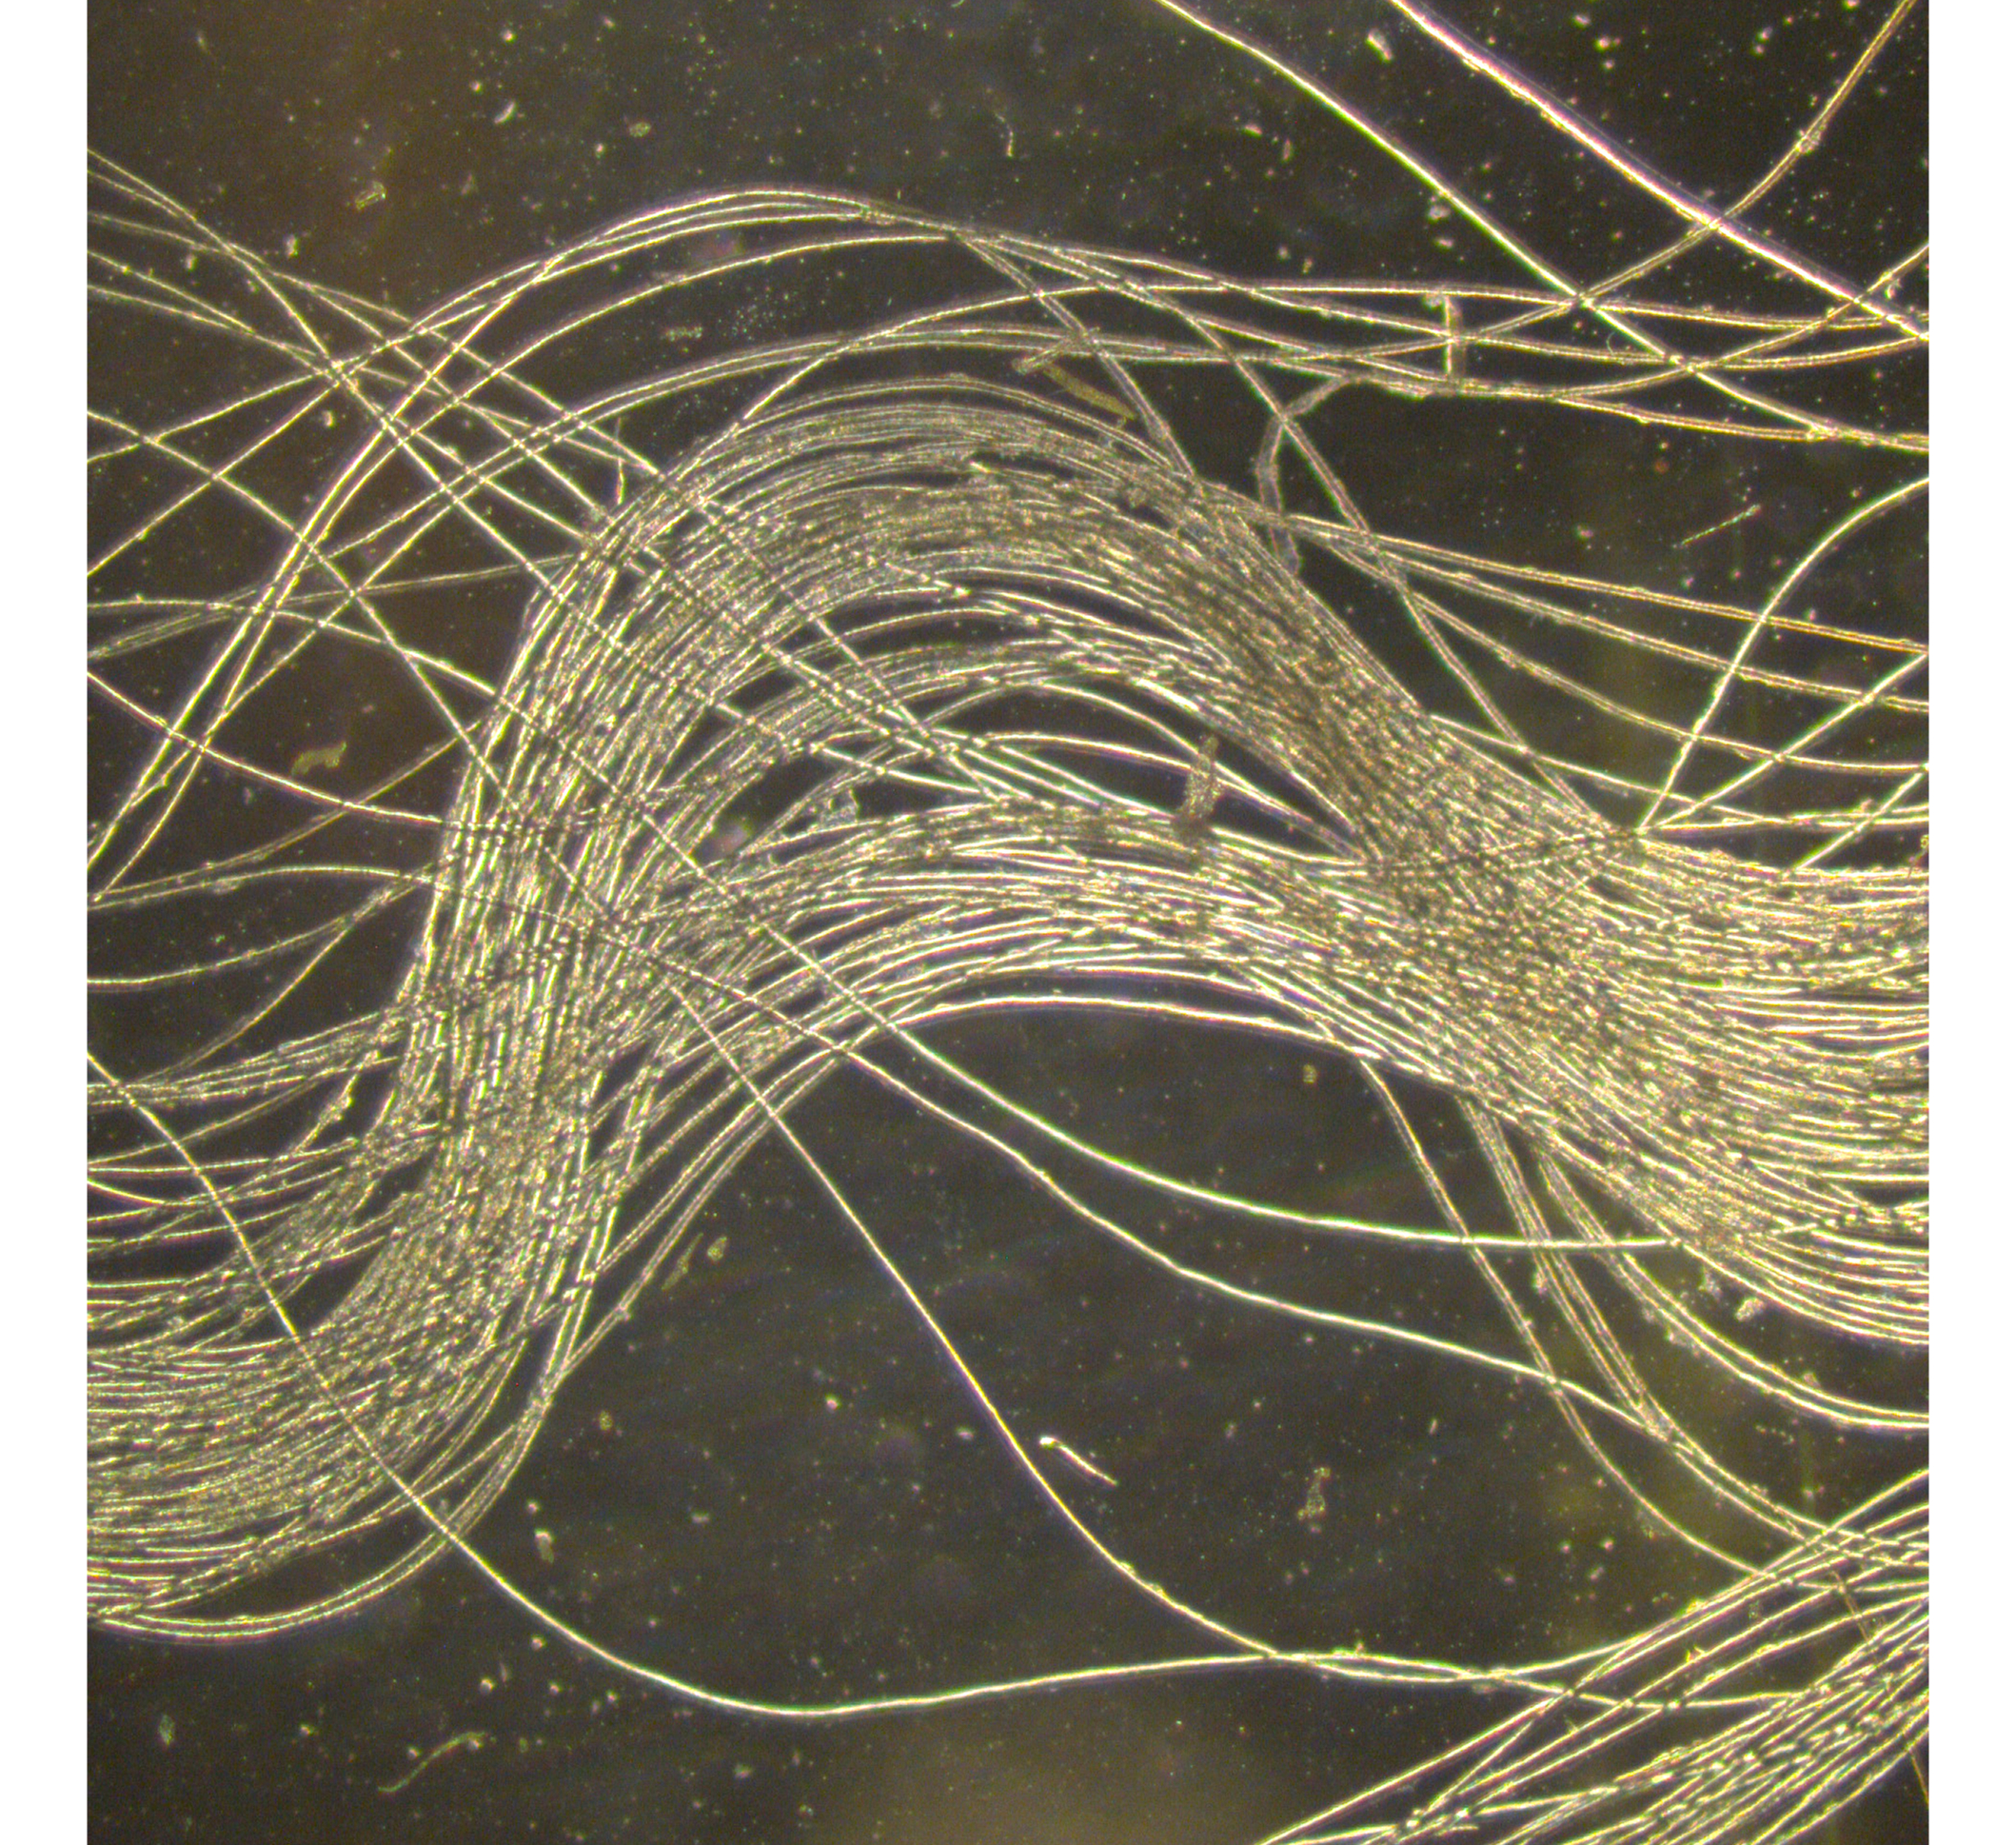
\includegraphics[width=1.0\textwidth]{figtwist.jpg}
  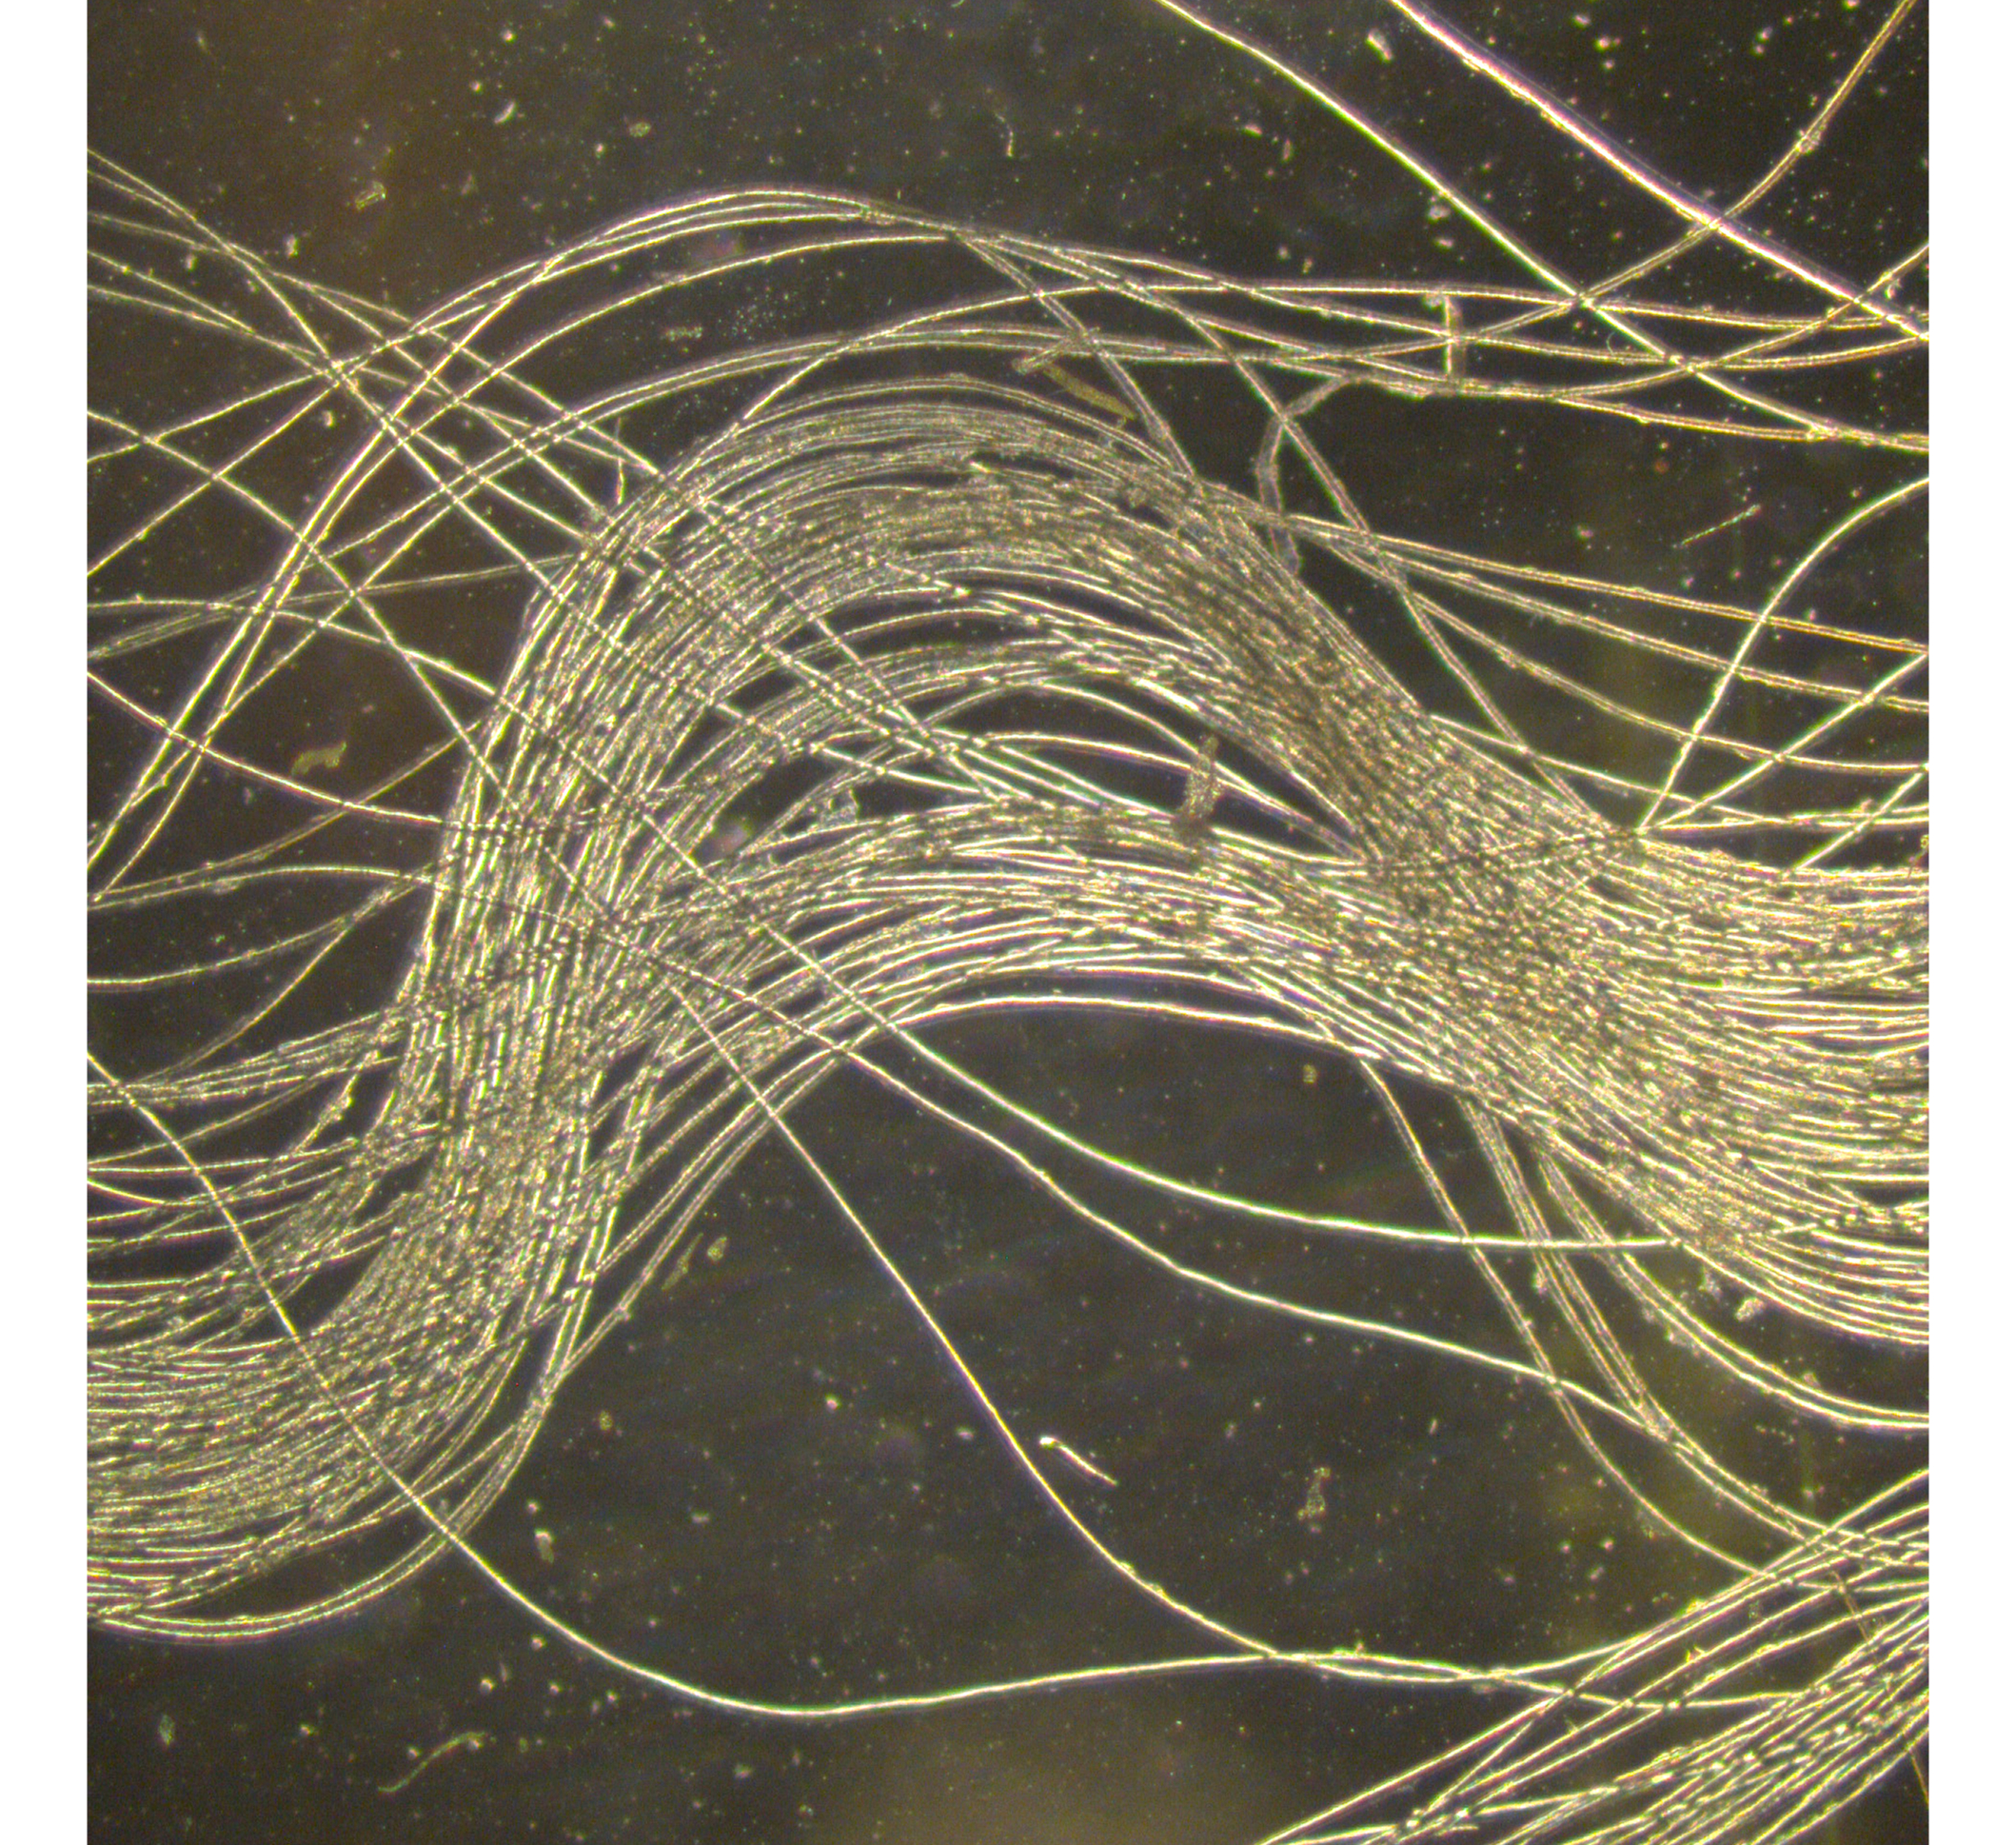
\includegraphics[scale=0.16]{figtwist.jpg}
%   unfo525.jpg is original photo on proj mic
  \caption{Photomicrograph, taken with phase contrast microscope, showing a bundle of fibres from a sheep with semicircular or horseshoe crimp. Note twisted fibres at each of the two points of inflection and absence of twist elsewhere. Note semicircular (non sine wave) shape of the crimp. Microscope magnification 25x. For printed or screen magnification see Appendix }
  \label{fig:twist}
\end{figure}

%\end{document}

  

It is difficult to determine the exact amount of twist, but it should be close to 180 degrees. If one looks carefully at the two twisted fibre regions in Figure~\ref{fig:twist} one can see that the fibres which pass over other fibres at the upper twist point pass under other fibres at the lower twist point.  The two successive twists are in opposite directions. The upper twist is anticlockwise (looked at from the bottom of the fibre bundle), and the lower twist is clockwise. This is a further confirmation of the appropriateness of the unfolding model - the wire model in Figure~\ref{fig:10} has the same alternate "S" and "Z" twists a seen in Figure~\ref{fig:twist}.

Figure~\ref{fig:notwist} shows a bundle of fibres from a sheep with dished sine wave crimp. There is no concentration of twist at any point along the wave. There are some unaligned fibres which cross over other fibres, but this occurs at all points along the wave and is not concentrated at the points of inflection.

%\documentclass{article}
%\usepackage{graphicx,subfigure}
%\begin{document}

\begin{figure}[!h]
  \centering
% 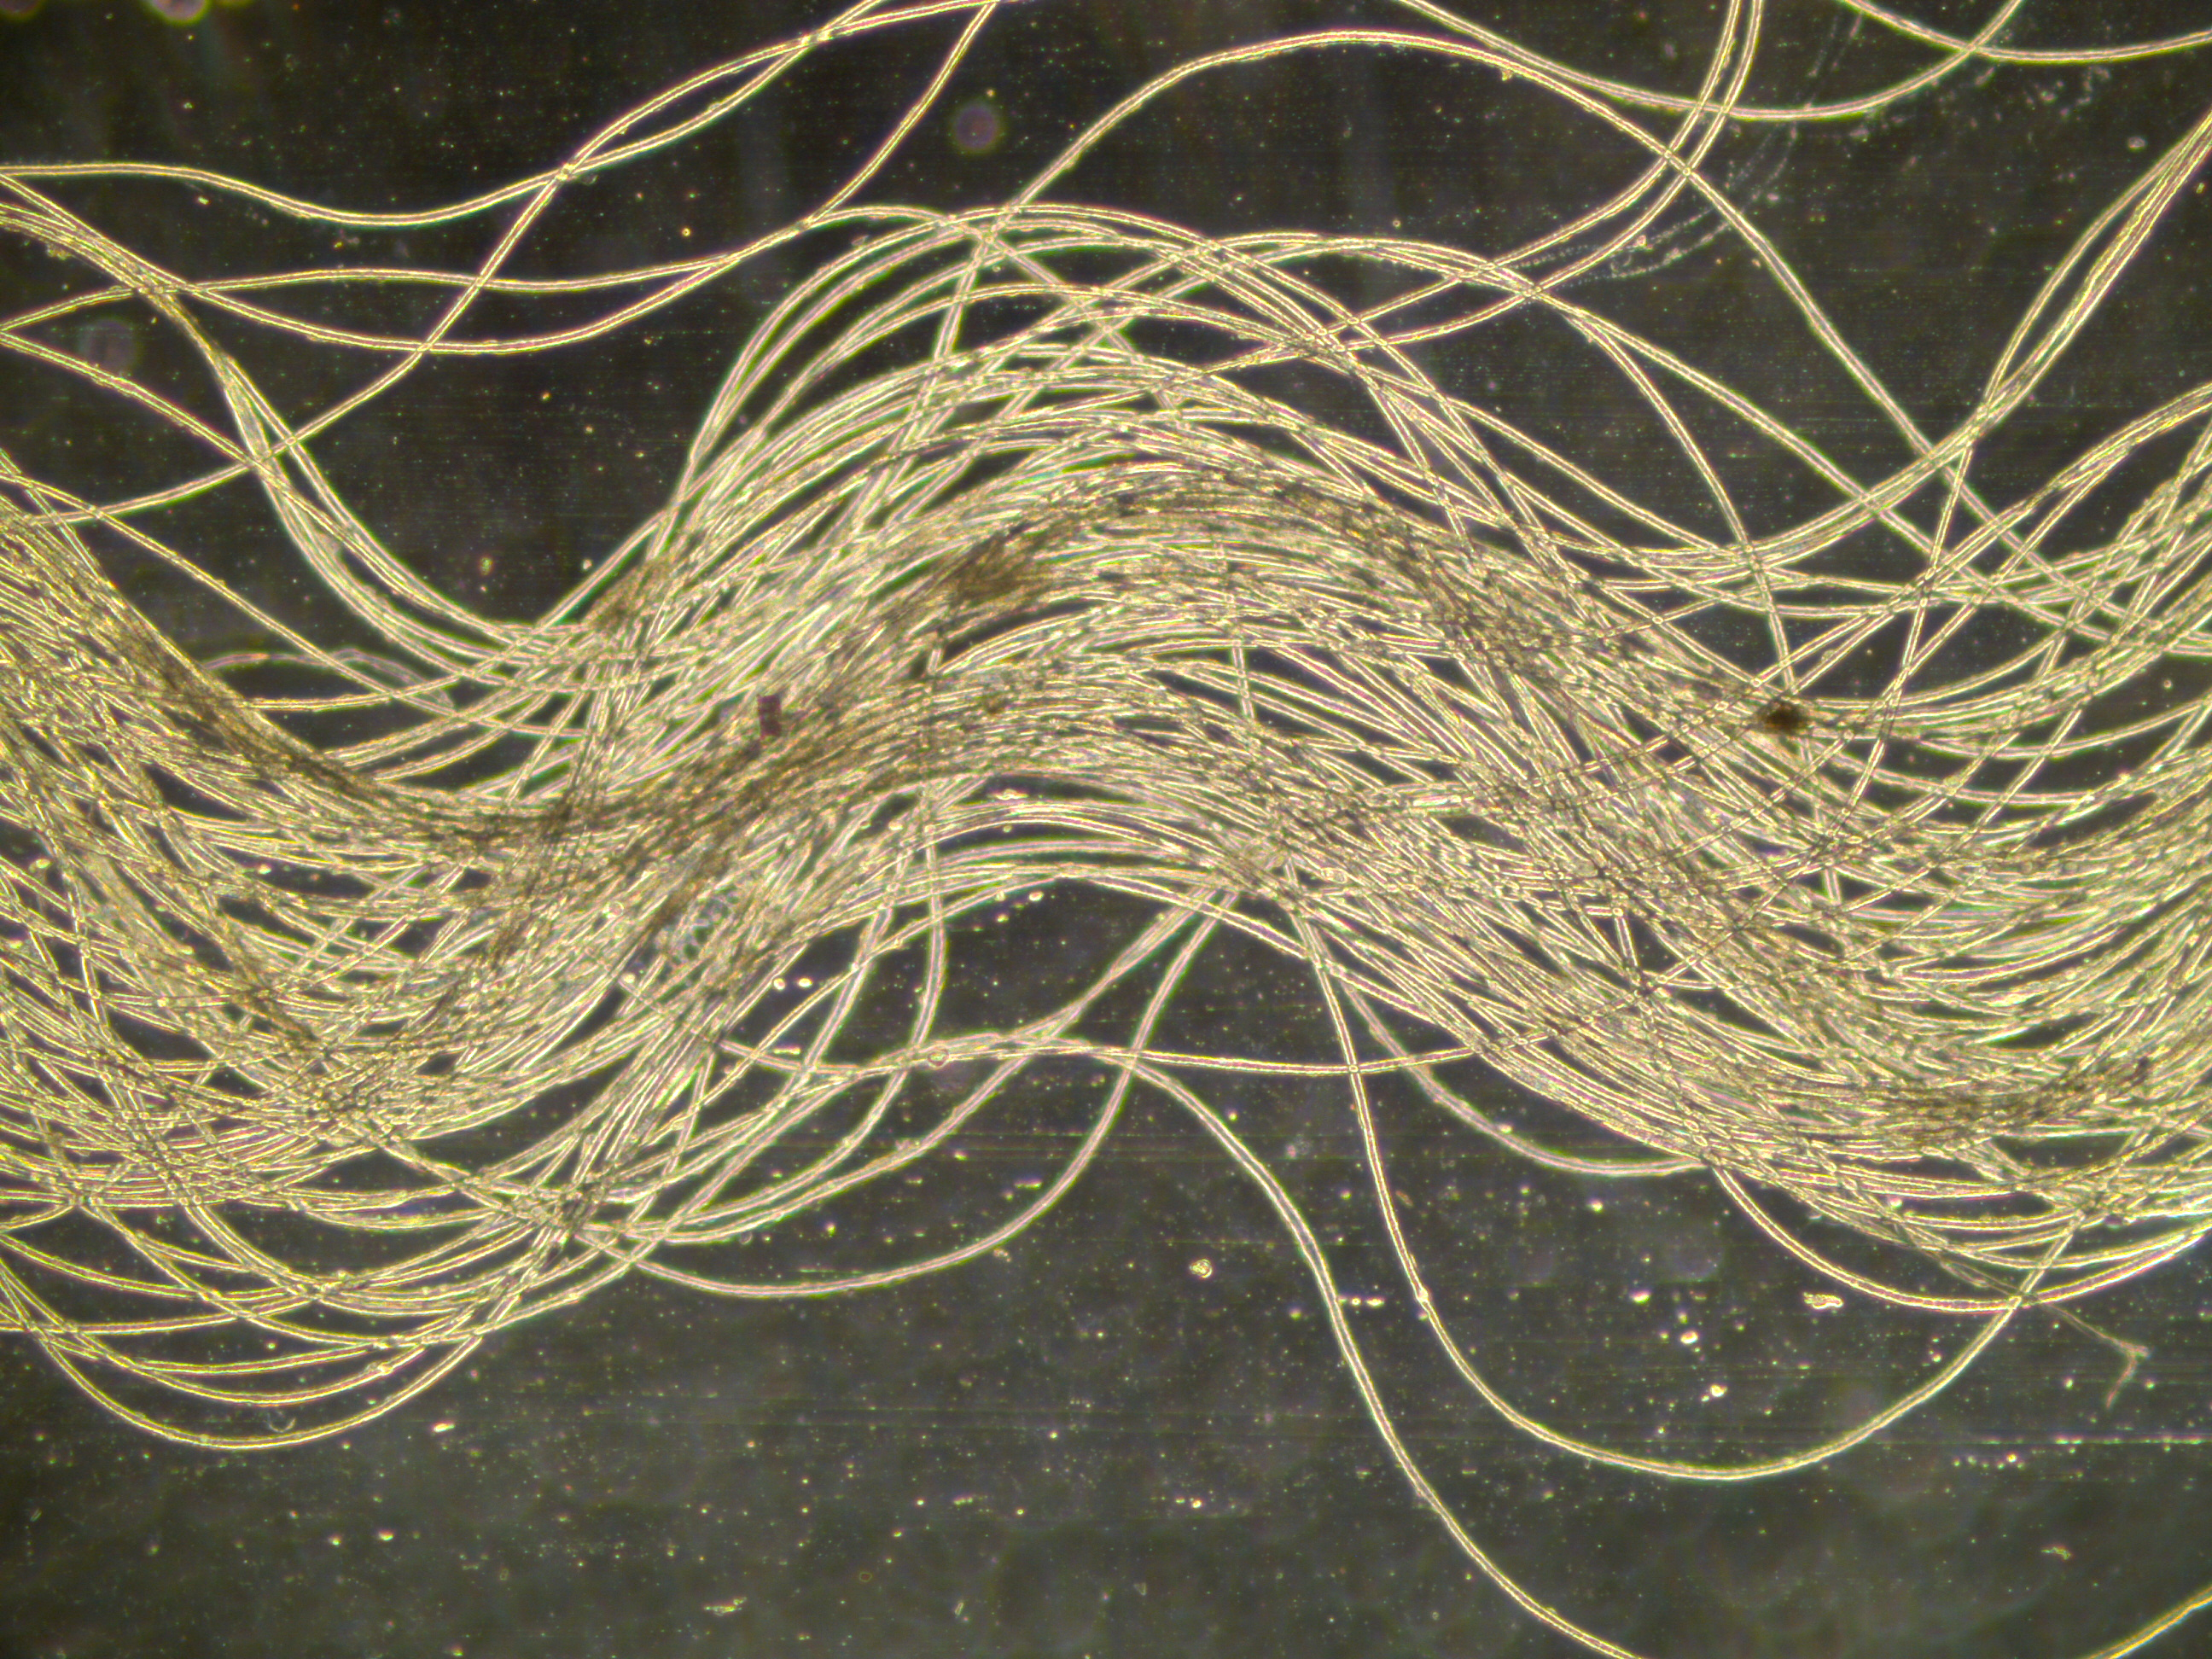
\includegraphics[width=1.0\textwidth]{fignotwist.jpg}
  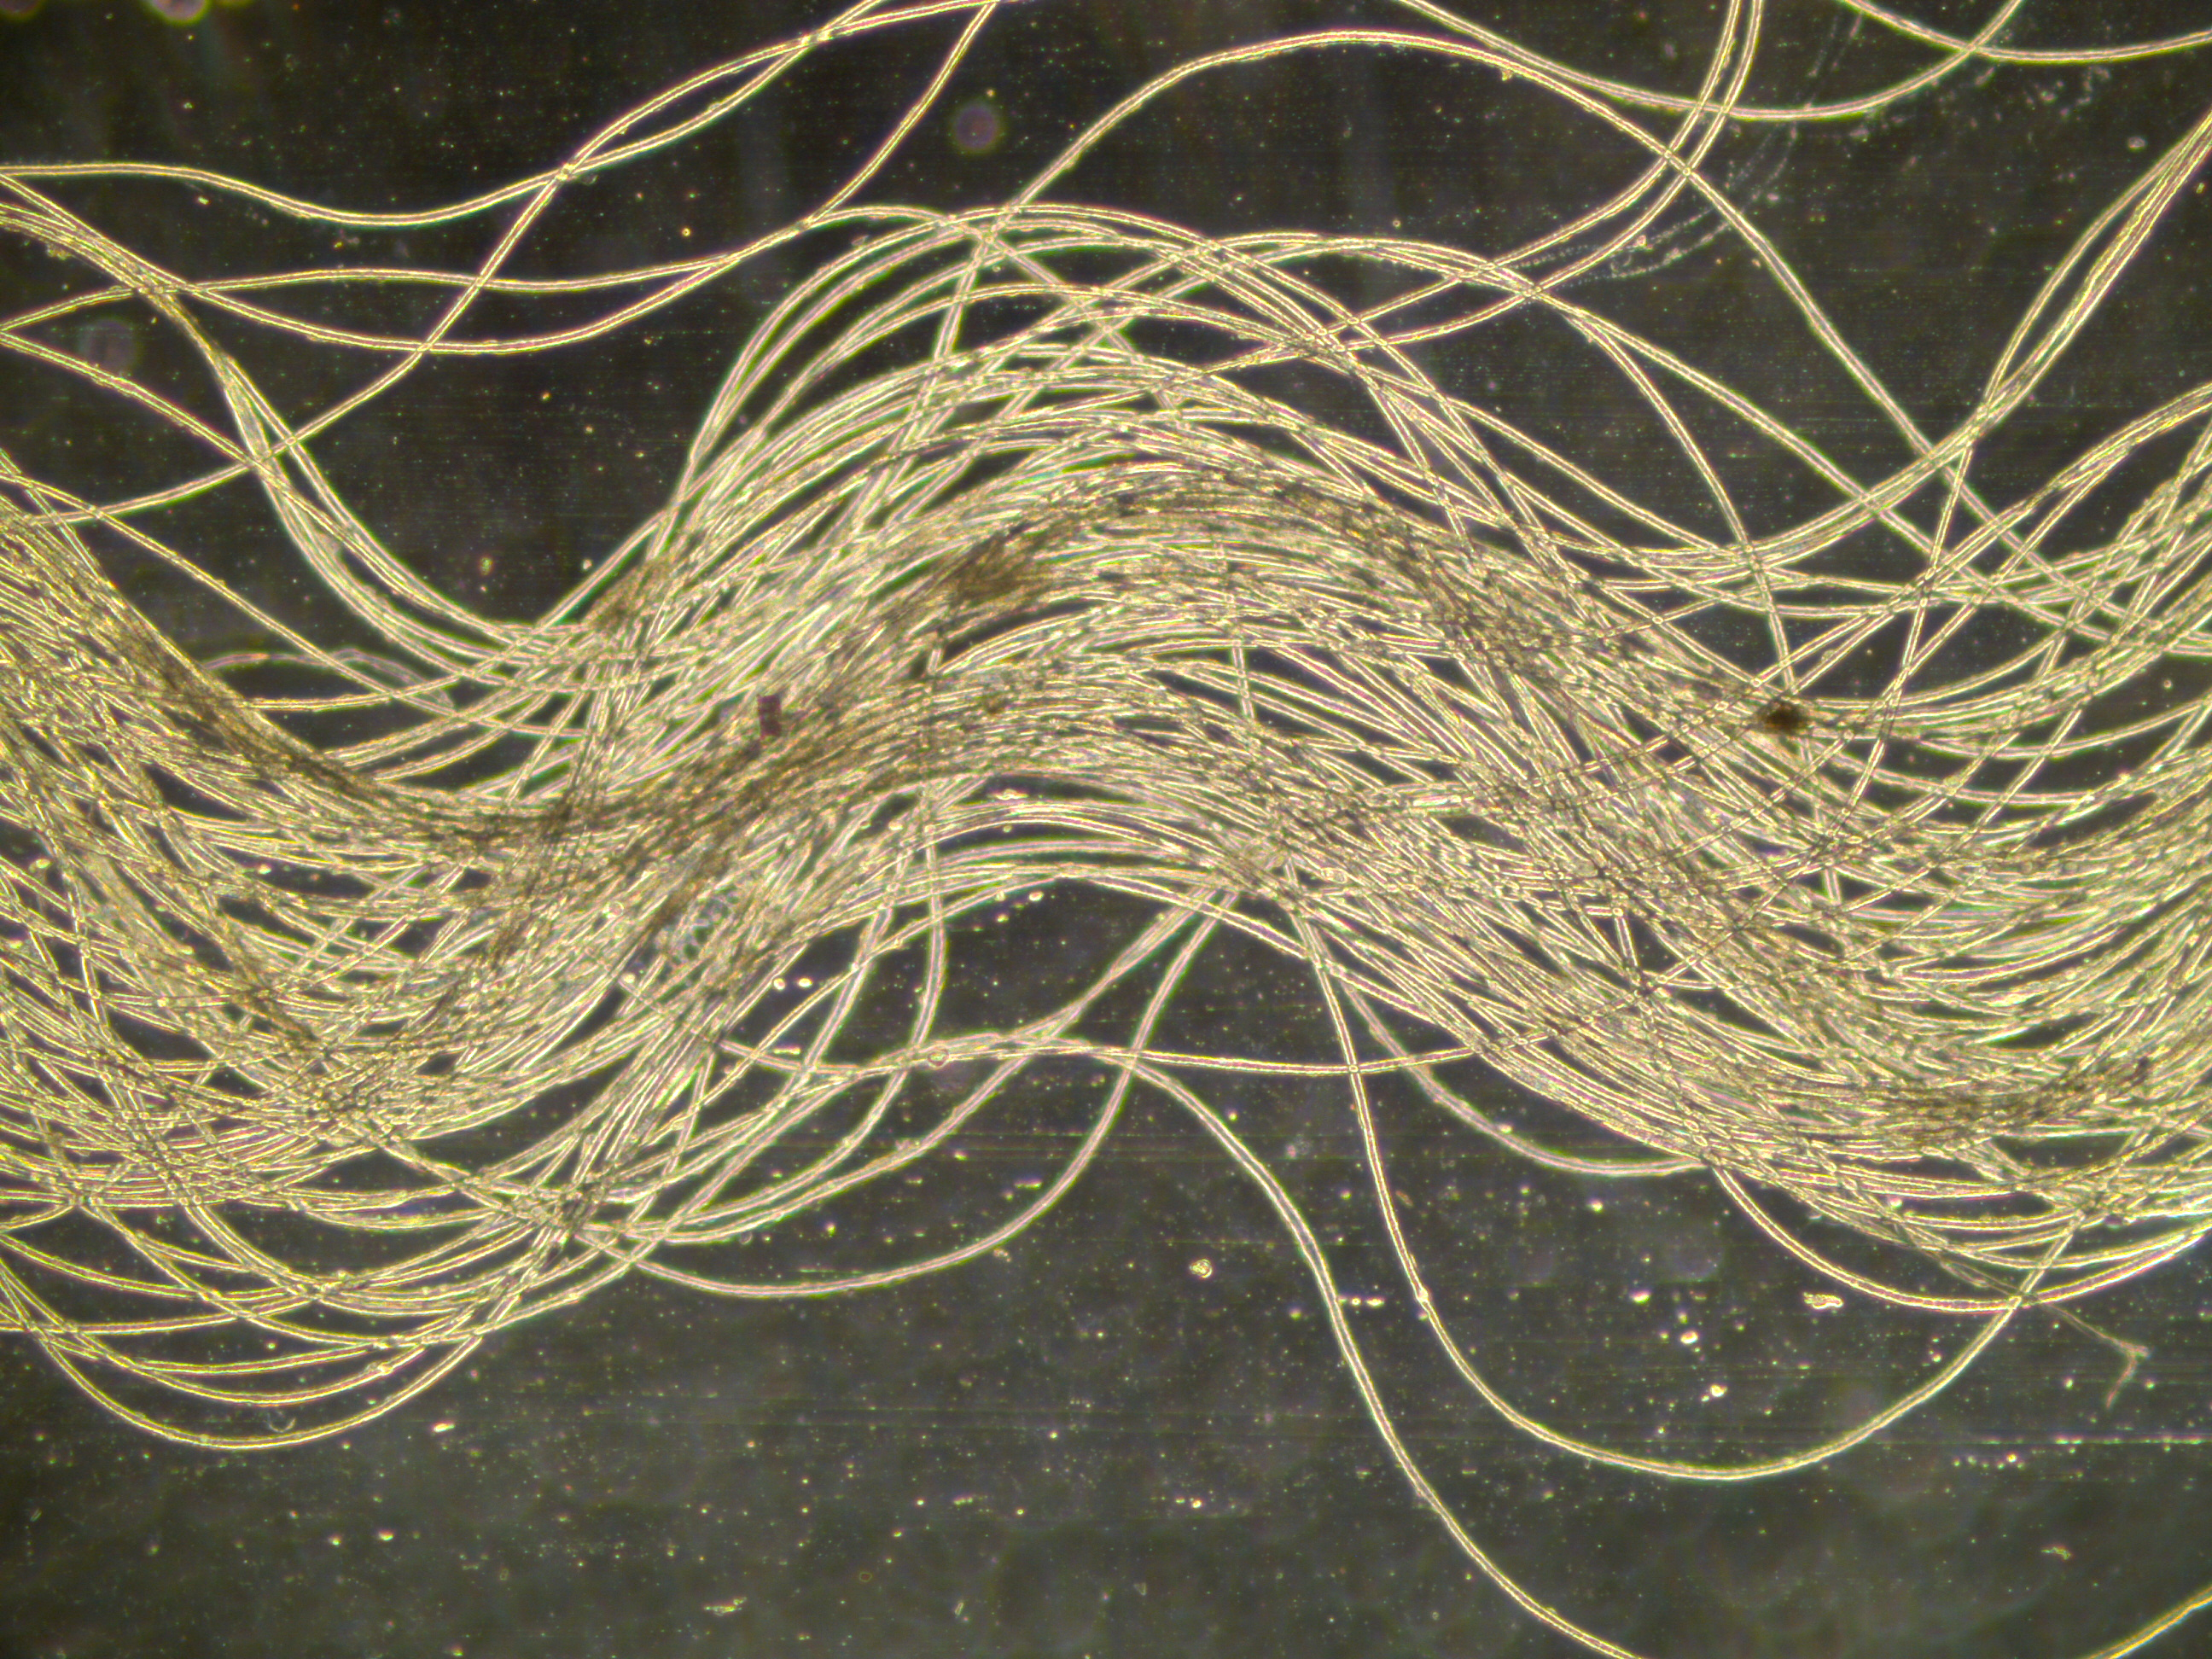
\includegraphics[scale=0.55]{fignotwist.jpg}
%   unalfib516.jpg is original photo on proj mic
  \caption{Photomicrograph, taken with phase contrast microscope, showing a bundle of fibres from a sheep with dished sine wave crimp. Note absence of twisted fibres at any point, and soma unaligned fibres which cross the other fibres at various points. Note sine wave shape of the crimp. Microscope magnification 25x. For printed or screen magnification see Appendix. }
  \label{fig:notwist}
\end{figure}

%\end{document}

  

Unaligned fibres are more common in sheep with dished sine wave crimp.

The two Figures also illustrate the different shape of the crimp wave for the two types of sheep. In Figure~\ref{fig:notwist} the fibres have a typical sine wave shape as produced by the stretched helix model. In Figure~\ref{fig:twist} the fibres have a semicircular shape as produced by the unfolded helix model.

We conclude that the basic correctness of our stretched helix and unfolded helix models has been verified, and that their applicability to wools with dished sine wave crimp and semicircular or horseshoe crimp has been tested and found reliable.


\subsection{Some further considerations regarding the conditions under which stretching or unfolding can occur}
\label{sec:further}
To understand why some fleeces form dished sine wave crimp and other fleeces form horseshoe or high amplitude crimp we need some insight into {\em how} these two different types of fibre arrangement can occur. Our static models with wires are just an abstract way of thinking about what is possible. No-one imagines that we actually have a compressed helix of fibres lying on the skin surface waiting to be either stretched or unfolded.  As noted in Section~\ref{sec:dyn} above the process is dynamic, and probably occures in the region 1-5 mm above the skin surface. After that the fibres are set into a particular crimp position, and little further rearrangement occurs, unless the fleece is disrupted by weathering.

So what happens in this 1-5 mm above the skin surface as the fibres grow out? For the stretched helix case it is relatively easy to envisage, at least in a qualitative way. The forces from the surrounding growing fibres simply lift a given fibre up at the points of fibre contact, turning the conceptual helix over so it is vertical to the skin,  and stretching it to produce a typical dished sine wave in the fibre. The stretching is probably helped by some fibres growing faster than the majority.  Once away from the skin surface, no additional forces occur, so the fibres take a set in whatever position they are in at that point.The final staple length achieved is actually a measure of the amount of stretch, and therefore of the amount of stretching force. The wavelength of the crimp (reciprocal of frequency) is probably a better index of the amount of stretching force as it is not dependent on fibre length growth rate, whereas staple length reflects both fibre length growth rate and stretching. 

There is one type of staple structure found in some Mohair strains and in British Wensleydale and Teeswater sheep which is called ringlets. Each ringlet is actually a helix in which there has been little or no stretching or unfolding. The fibres are always well aligned so that bundles of fibres forming a coordinated set of ringlets become the staple. This type of fleece provides a clear demonstration that our assumption of an unstretched helix as the stating point of all crimp formation is correct.  

For the unfolded helix case, we have more difficulty envisaging the action. Unfolding of a helix is a much more complex phenomenon than stretching. Each loop of the helix has to be turned (rotated) sideways out of the helix cylinder, the first loop clockwise, the second anticlockwise, the third clockwise again, ... The result is an alternate S and Z twisting of fibre bundles at the points of inflection. So in contrast to a stretched helix, which is a single fibre phenomenon ( or all fibres up to a whole staple if you like), an unfolded helix is a phenomenon which can only occur with groups of fibres (called bundles). We think that these bundles actually represent the cluster of fibres produced by a follicle group.
 Exactly what sort of forces cause this alternating unfolding (and associated twisting of fibres in each bundle) is not easy to envisage. They are obviously lateral forces (across the helix cylinder) because the succesive loops are turned sideways ( rather than stretched longitudinally).

One of the most puzzling aspects of unfolded helix crimp is the concentration of twisted fibres in each bundle at the points of inflection of the crimp wave. The fibres are never twisted at the peak or trough of the wave. For twist to occur at one point only, the fibre bundle must be held. The only obvious place where the bundle is held, is where the follicles of the follicle group hold the fibres - ie right at the skin surface.

The next most puzzling issue is that an unfolding requires space beside the helix for the successive loops to unfold into. This is different from a stretching, which requires no lateral space, and actually reduces the lateral dimension of the helix slightly. So where does this space come from? Sheep with a well formed horseshoe crimp ( such as SRS \textsuperscript{TM} Merinos) have their follicle groups arranged in the skin in rows, with bands of connective tissue between the rows. Figure~\ref{skin:hs} shows this clearly. This phenomenon was first noted by Nay(1966)~\cite{nay:66}. We will adopt a convention of calling the sides of each follicle group adjacent to connective tissue north and south, and the other two sides adjacent to other follicle groups east and west. Figure~\ref{skin:hs} is oriented in this manner. The space for loops to unfold comes from  the connective tissue space on the north and south sides of the follicle groups. On the east and west sides of each follicle group there are dense growths of fibres from the adjoining follicle groups. Each follicle group grows a bundle of fibres. The fibre contacts around this bundle will be asymmetric - dense on the east and west sides, sparse on the north and south sides.

%\documentclass{article}
%\usepackage{graphicx,subfigure}
%\begin{document}

\begin{figure}[!h]
  \centering
  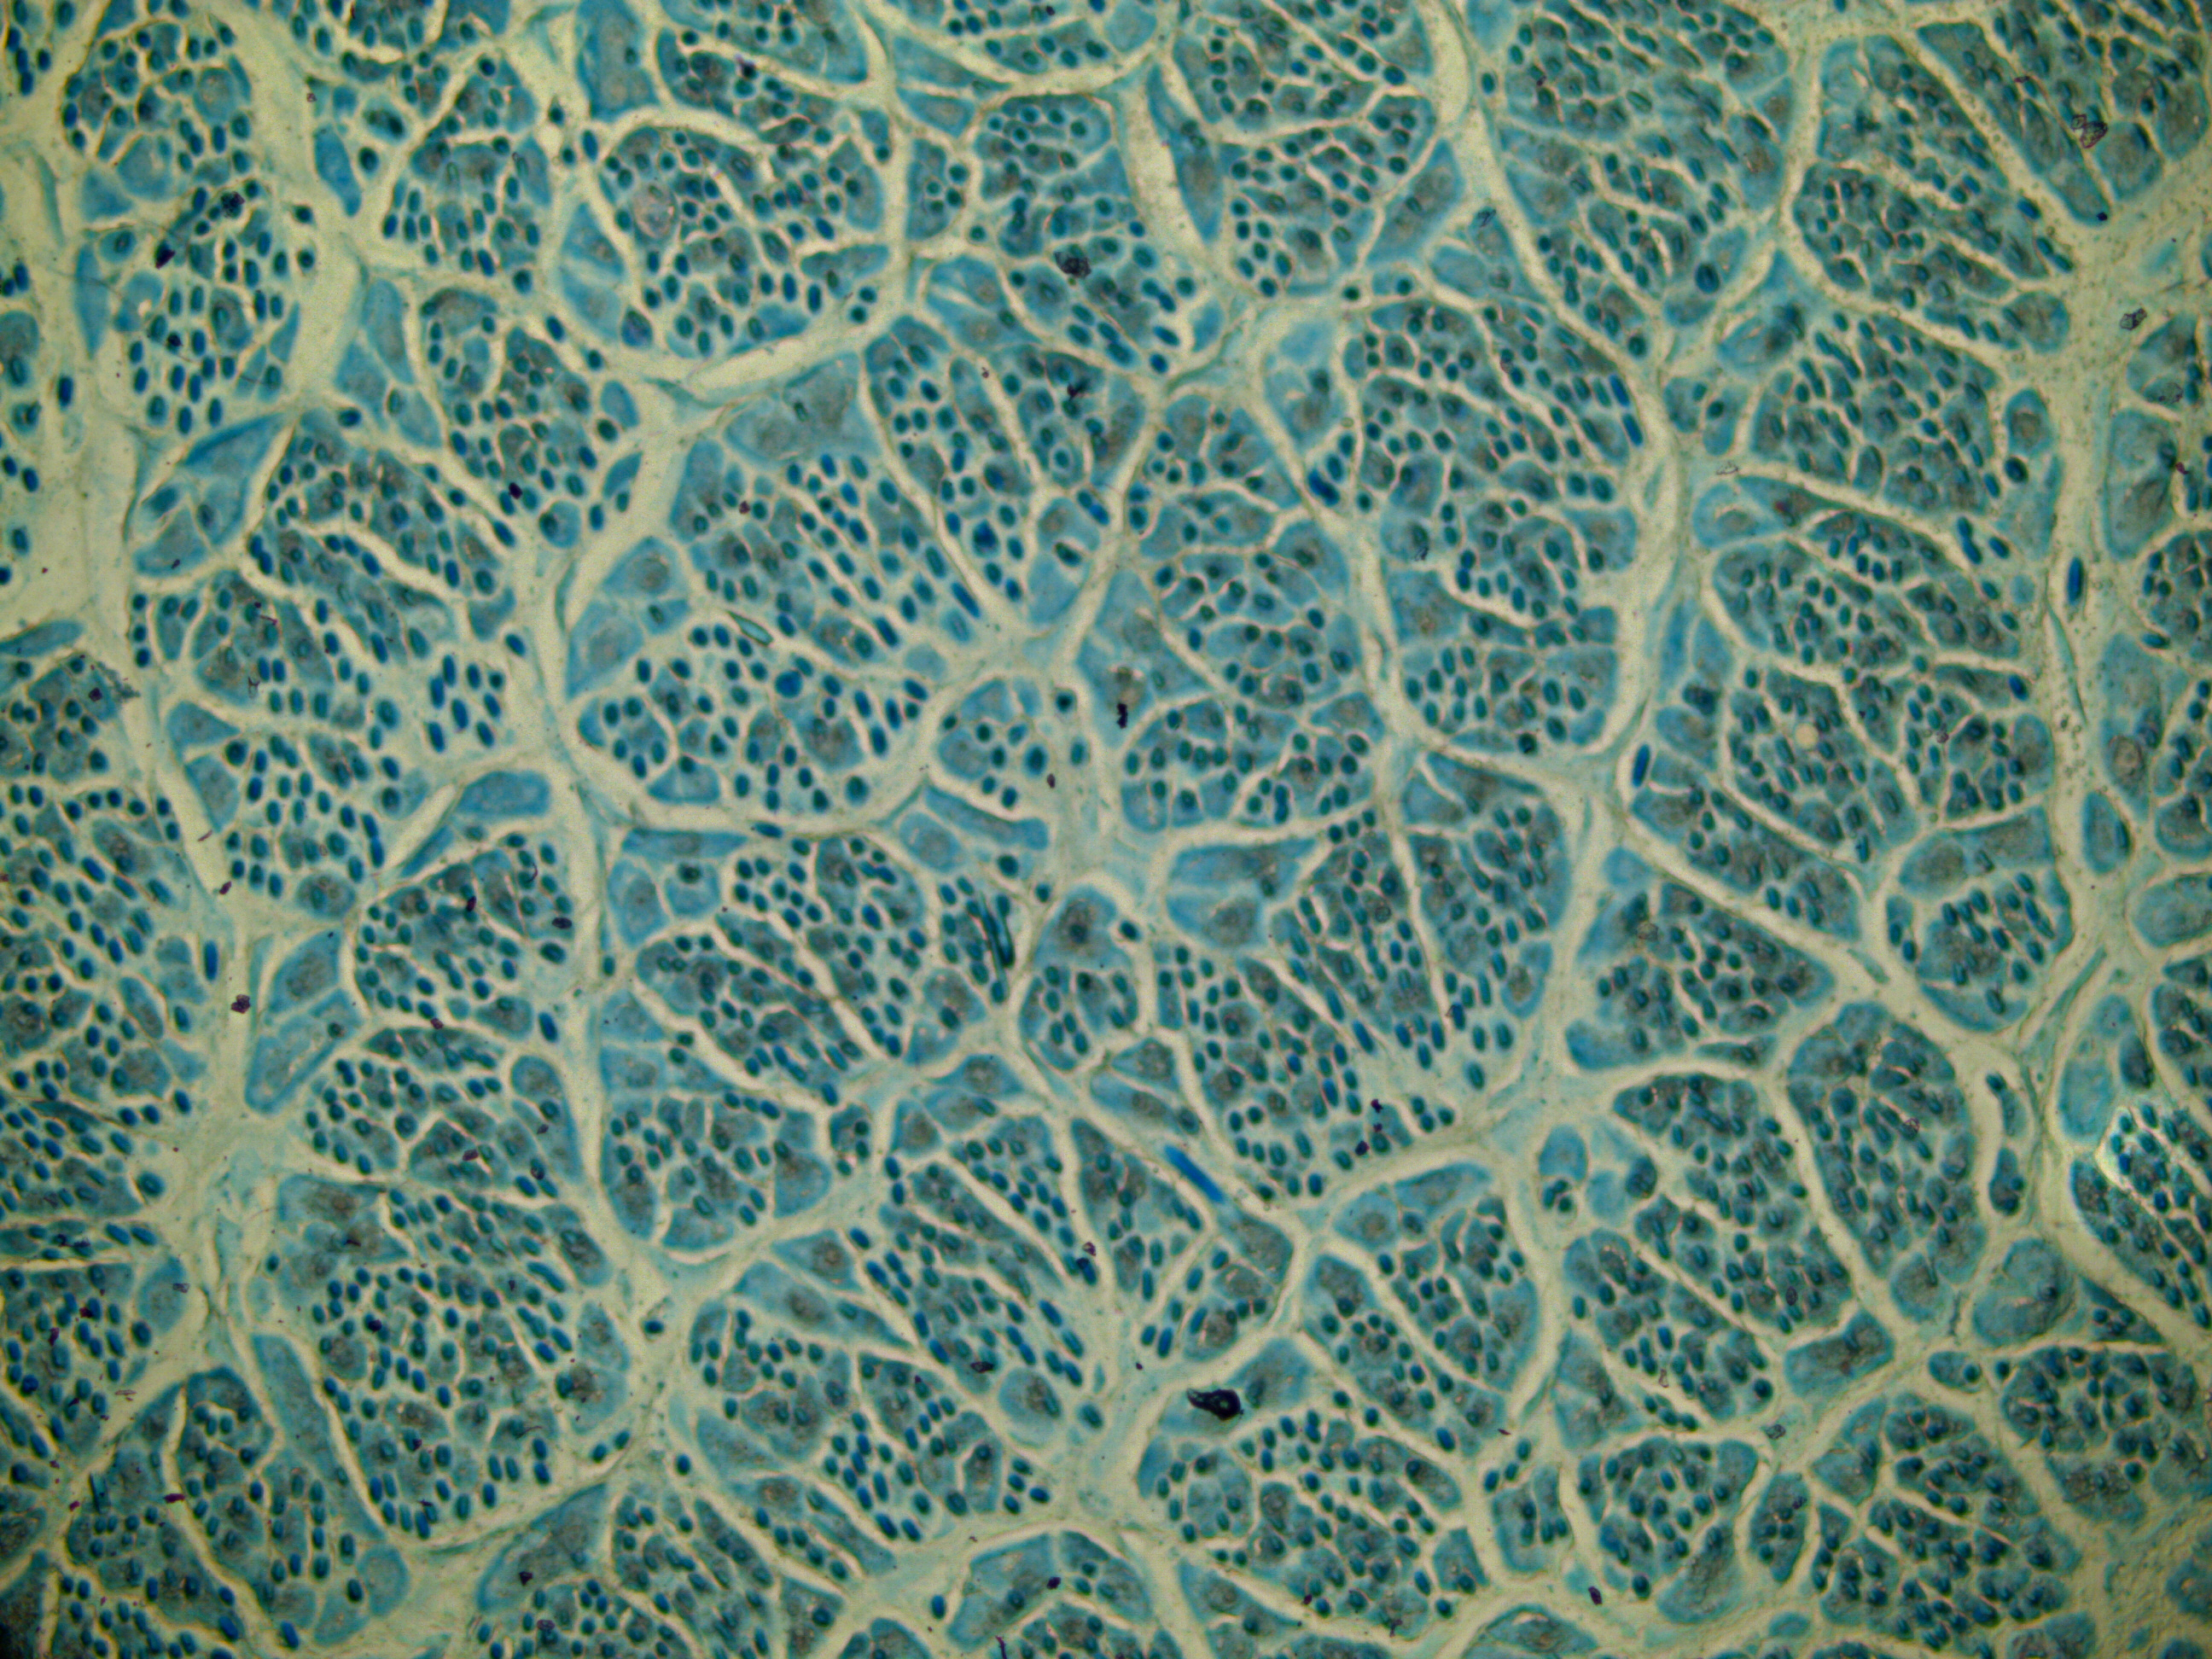
\includegraphics[width=1.0\textwidth,angle=90]{figskinhs.jpg}
% 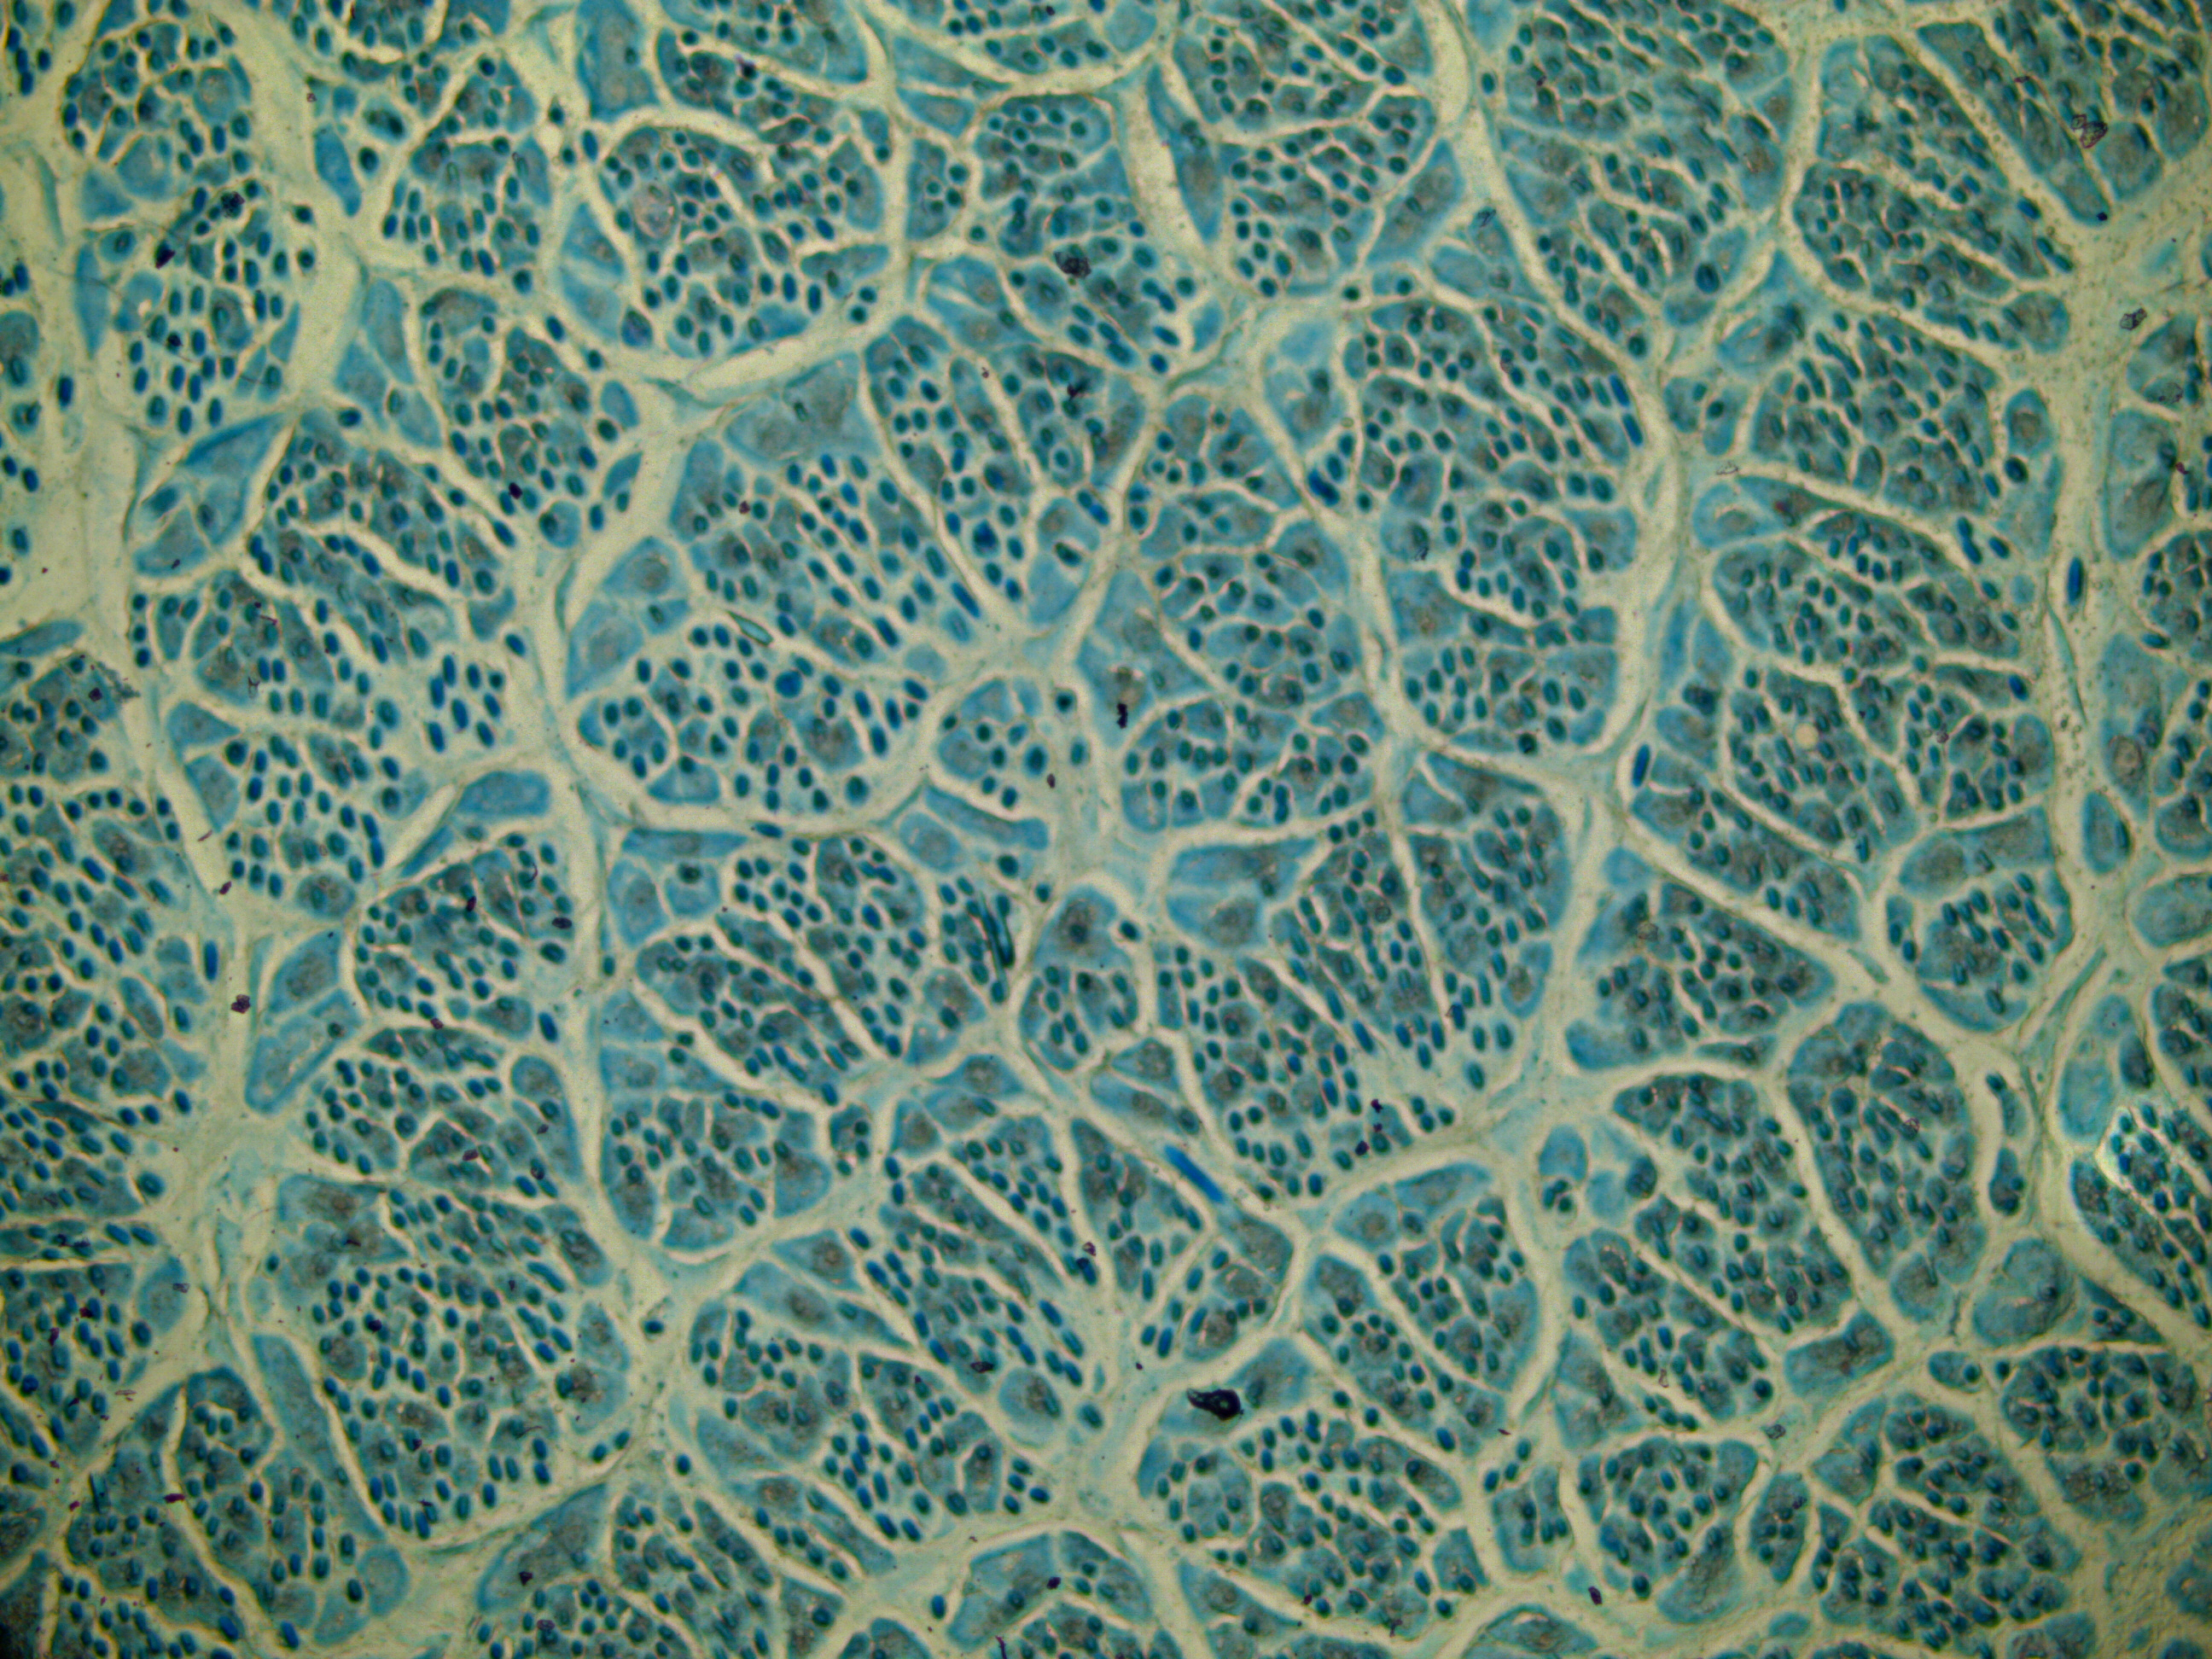
\includegraphics[width=1.0\textwidth]{figskinhs.jpg}
% 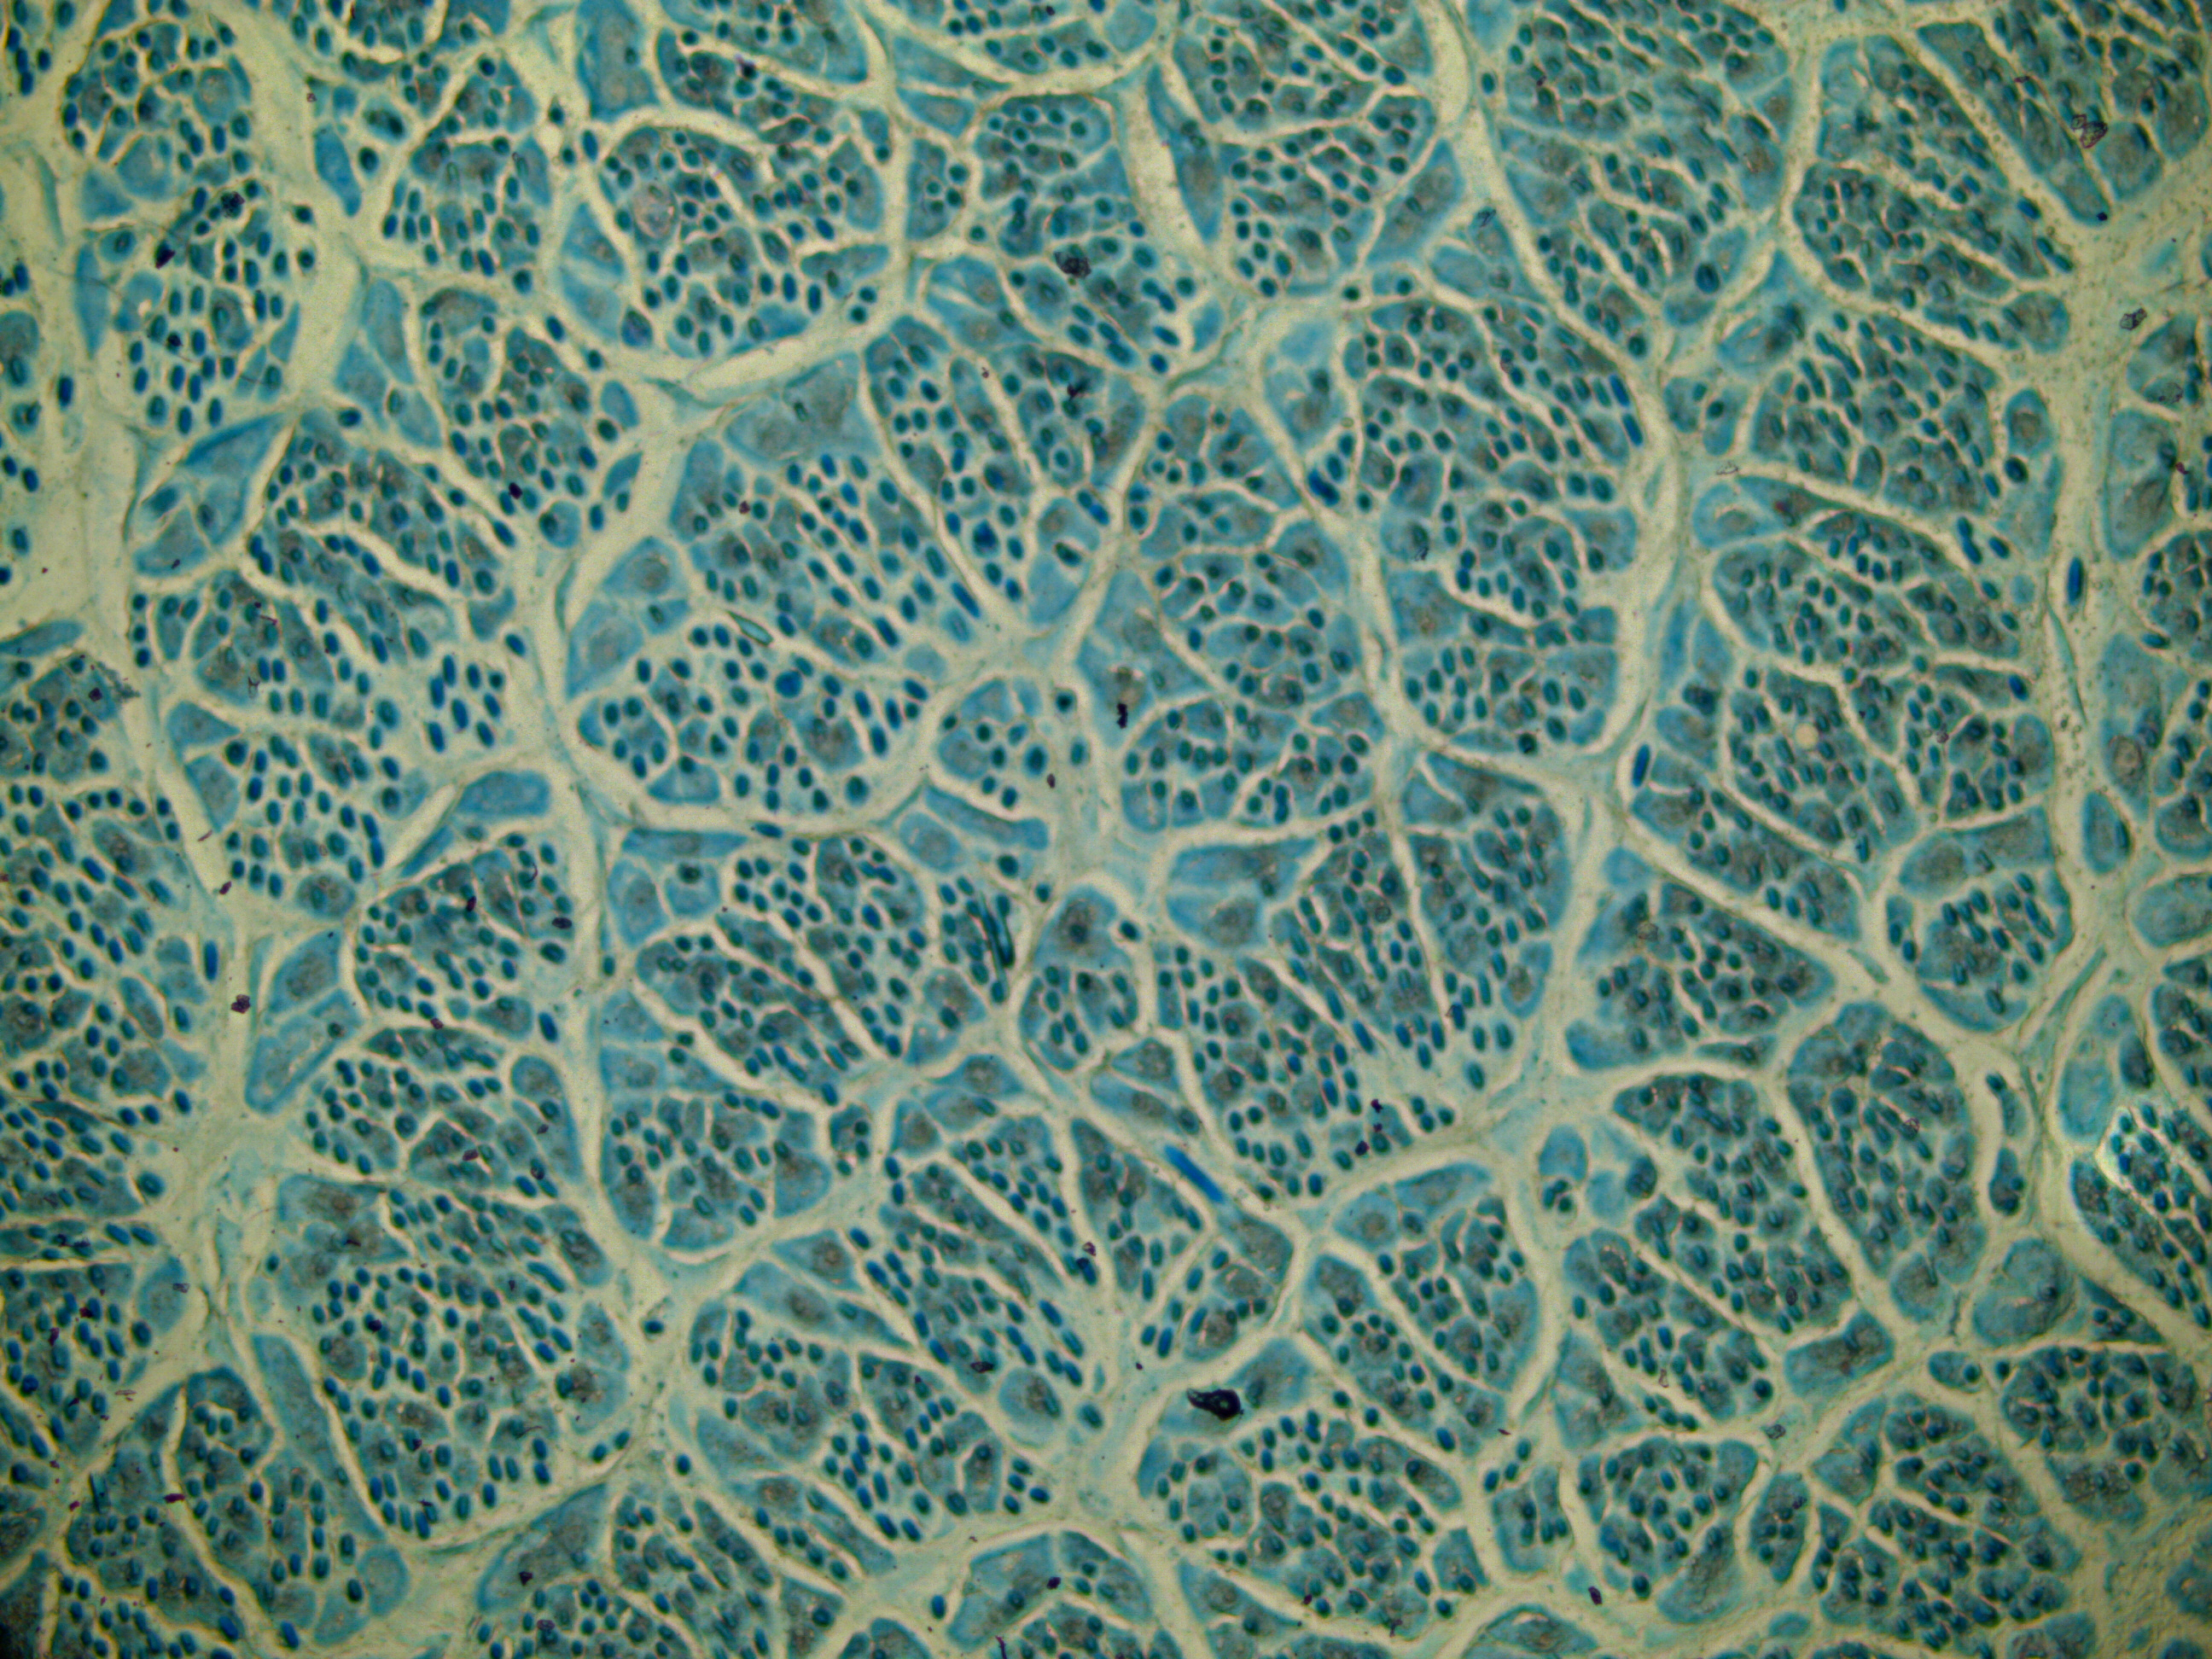
\includegraphics[scale=0.18]{figskinhs.jpg}
  \caption{A horizontal skin section from a Merino sheep with unfolded helix crimp showing rows of follicle groups with appreciable connective tissue space between the rows. The direction referred to as north-south is vertical and east-west is horizontal. 25x magnification. Stained with Nile Blue sulphate}
  \label{skin:hs}
\end{figure}

%\end{document}



So, imagine a bundle of growing fibre tips coming out of a follicle group in a curved path. They will eventually encounter an obstacle provided by dense fibres on the east or west side of the follicle group. The loop of growing fibres will then take the path of least resistance and slew into the north or south side space. When the loop slews, say to the north side, it causes twist, and this twist runs down the bundle to the skin surface, where it stops. A sideways slew will only give up to 90 degrees of twist. We illustrate this in Figure~\ref{twist1}.
 
%\documentclass{article}
%\usepackage{graphicx,subfigure}
%\begin{document}

\begin{figure}[!h]
  \centering
  \includegraphics[width=1.1\textwidth]{fig13bfilt.png}
  \caption{A drawing showing the first loop of a growing bundle of fibres slewing to the right on encountering a dense fibre barrier in the direction of fibre curvature. A 90 degree twist occurs at the skin surface.}
  \label{twist1}
\end{figure}

%\end{document}



So, what happens next? Well, the loop fills the north side space. The fibre bundle keeps growing, and the next loop can not use the north side space because it is filled, so it slews the opposite way (again the path of least resistance) into the south side space. This slew, of the second loop, causes two twists, one at the skin surface (up to minus 90 degrees this time) and one (up to plus 90 degrees) at the point of the previous twist, which has now grown up by half a wavelength. So the previous twist acts as a second holding point. Now there are two 90 degrees twists at that point, adding to 180 degrees of unfolding or twist. We illustrater this in Figure~\ref{twist2}.

%\documentclass{article}
%\usepackage{graphicx,subfigure}
%\begin{document}

\begin{figure}[!h]
  \centering
  \includegraphics[width=1.1\textwidth]{fig14bfilt.png}
  \caption{A drawing showing the second loop of a growing bundle of fibres slewing to the left causing 90 degree twists at the skin surface and at the position of the previous twist}
  \label{twist2}
\end{figure}

%\end{document}



The process continues in the same way with successive loops alternating beteen a 90 degree clockwise slew and a minus 90 degree anticlockwise slew. So the mystery of alternating lateral forces is explained - the only force is that created by the growing fibres. The absence of resistance to lateral movement of the loops allows this force to resolve in a lateral direction. The lateral directions alternate because of the serial nature of the process.

What we now need to explain is how does this line up with our wire model of unfolding where successive loops were unfolded 180 degrees and minus 180 degrees. The answer is that there are two ways of unfolding a helix
\begin{itemize}
\item alternate 180 degrees and minus 180 degrees unfoldings of successive loops with the unfolded end free to move
\item alternate 90 degrees and minus 90 degrees unfoldings of successive loops with the unfolded end held in a fixed position
\end{itemize}

They both result in the same unfolded helix, and both are mathematically equivalent, but it is clear that the latter is what happens on the sheep. The tip ends of fibre bundles are not free to wave around in a growing staple.

Understanding the space requirement and forces for unfolding to occur also adds to our understanding of stretched helix crimp. If the distribution of follicles and fibres around a  given follicle and its fibre are uniform or random, there is no direction of least resistance for sideways slewing, and the forces created by the growing fibre are simply resolved upwards resulting in a stretched helix. Wools with a dished sine wave crimp will therefore have an unstructured spatial distribution of follicles and fibre contacts.

We can now make some definitive statements as to what conditions are important for unfolding to occur
\begin{itemize}
\item follicle group arrangement and spacing
\item well aligned fibres in bundles
\item standard deviation of fibre length low ( no stretching and well aligned fibres)
\item perhaps high lustre (not too much friction between fibres)
\end{itemize}

We are also able to make some predictions which if observed may serve as a verification of the above
\begin{itemize}
\item   in an unfolded helix wool there should be up to 90 degrees of twist at the skin surface ( the exact amount depending on how far the loop has grown and slewed when viewed) and there should be close to 180 degrees of twist at every other point of inflection
\item in an unfolded helix wool the fibres in each bundle at the peaks and troughs of the wave should be moved apart an amount approximately equal to the thickness of the bundle. This will occur because  in slewing a loop to one side the fibres on that side of the bundle can move further over than the fibres on the opposite side of the bundle, leading to an increased separation
\item in an unfolded helix wool the plane of the unfolded wave should be north-south across the rows of follicle groups
\item in a stretched helix wool with well aligned fibres the above twists and separations will not occur 
\item in a stretched helix wool with poorly aligned fibres all  the fibres will appear as  individual stretched helices with little coordination into a visible staple crimp
\item in any stretched helix wool the spatial distribution of follicles and the consequent spatial distibution of fibre contacts in the 1-5 mm space above the skin will be close to uniform
\item in a wool with ringlets there will be no twist and no stretch of either bundles or individual fibres
\end{itemize}

\subsection{Evidence supporting our ideas regarding the conditions under which stretching or unfolding can occur}
\label{sec:evid2}

A number of additional predictions have been made concerning the factors which will differ between wools with dished sine wave crimp and semicircular or horseshoe crimp. To examine these, we need first to define these two types of crimp from the point of view of how they can be recognised from a visual examination of wool staples.

We actually define three types of staple crimp

\begin{description}
\item[unaligned] wools with a dished sine wave crimp that is made indistinct by an excess of poorly aligned fibres
\item[stretched] wools with a well defined dished sine wave crimp not obscured by poor fibre alignment
\item[unfolded] wools with a semicircular or horseshoe crimp. Fibre alignment in this type is always good
\end{description}

Figure~\ref{fig:woolphoto} shows three Merino wool staples illustrating the above three types. Figure~\ref{fig:fibre3types} shows photomicrographs of multiple bundles of fibres for each of the above three types.
%\documentclass{article}
%\usepackage{graphicx,subfigure}
%\begin{document}

\begin{figure}[!h]
  \centering
% 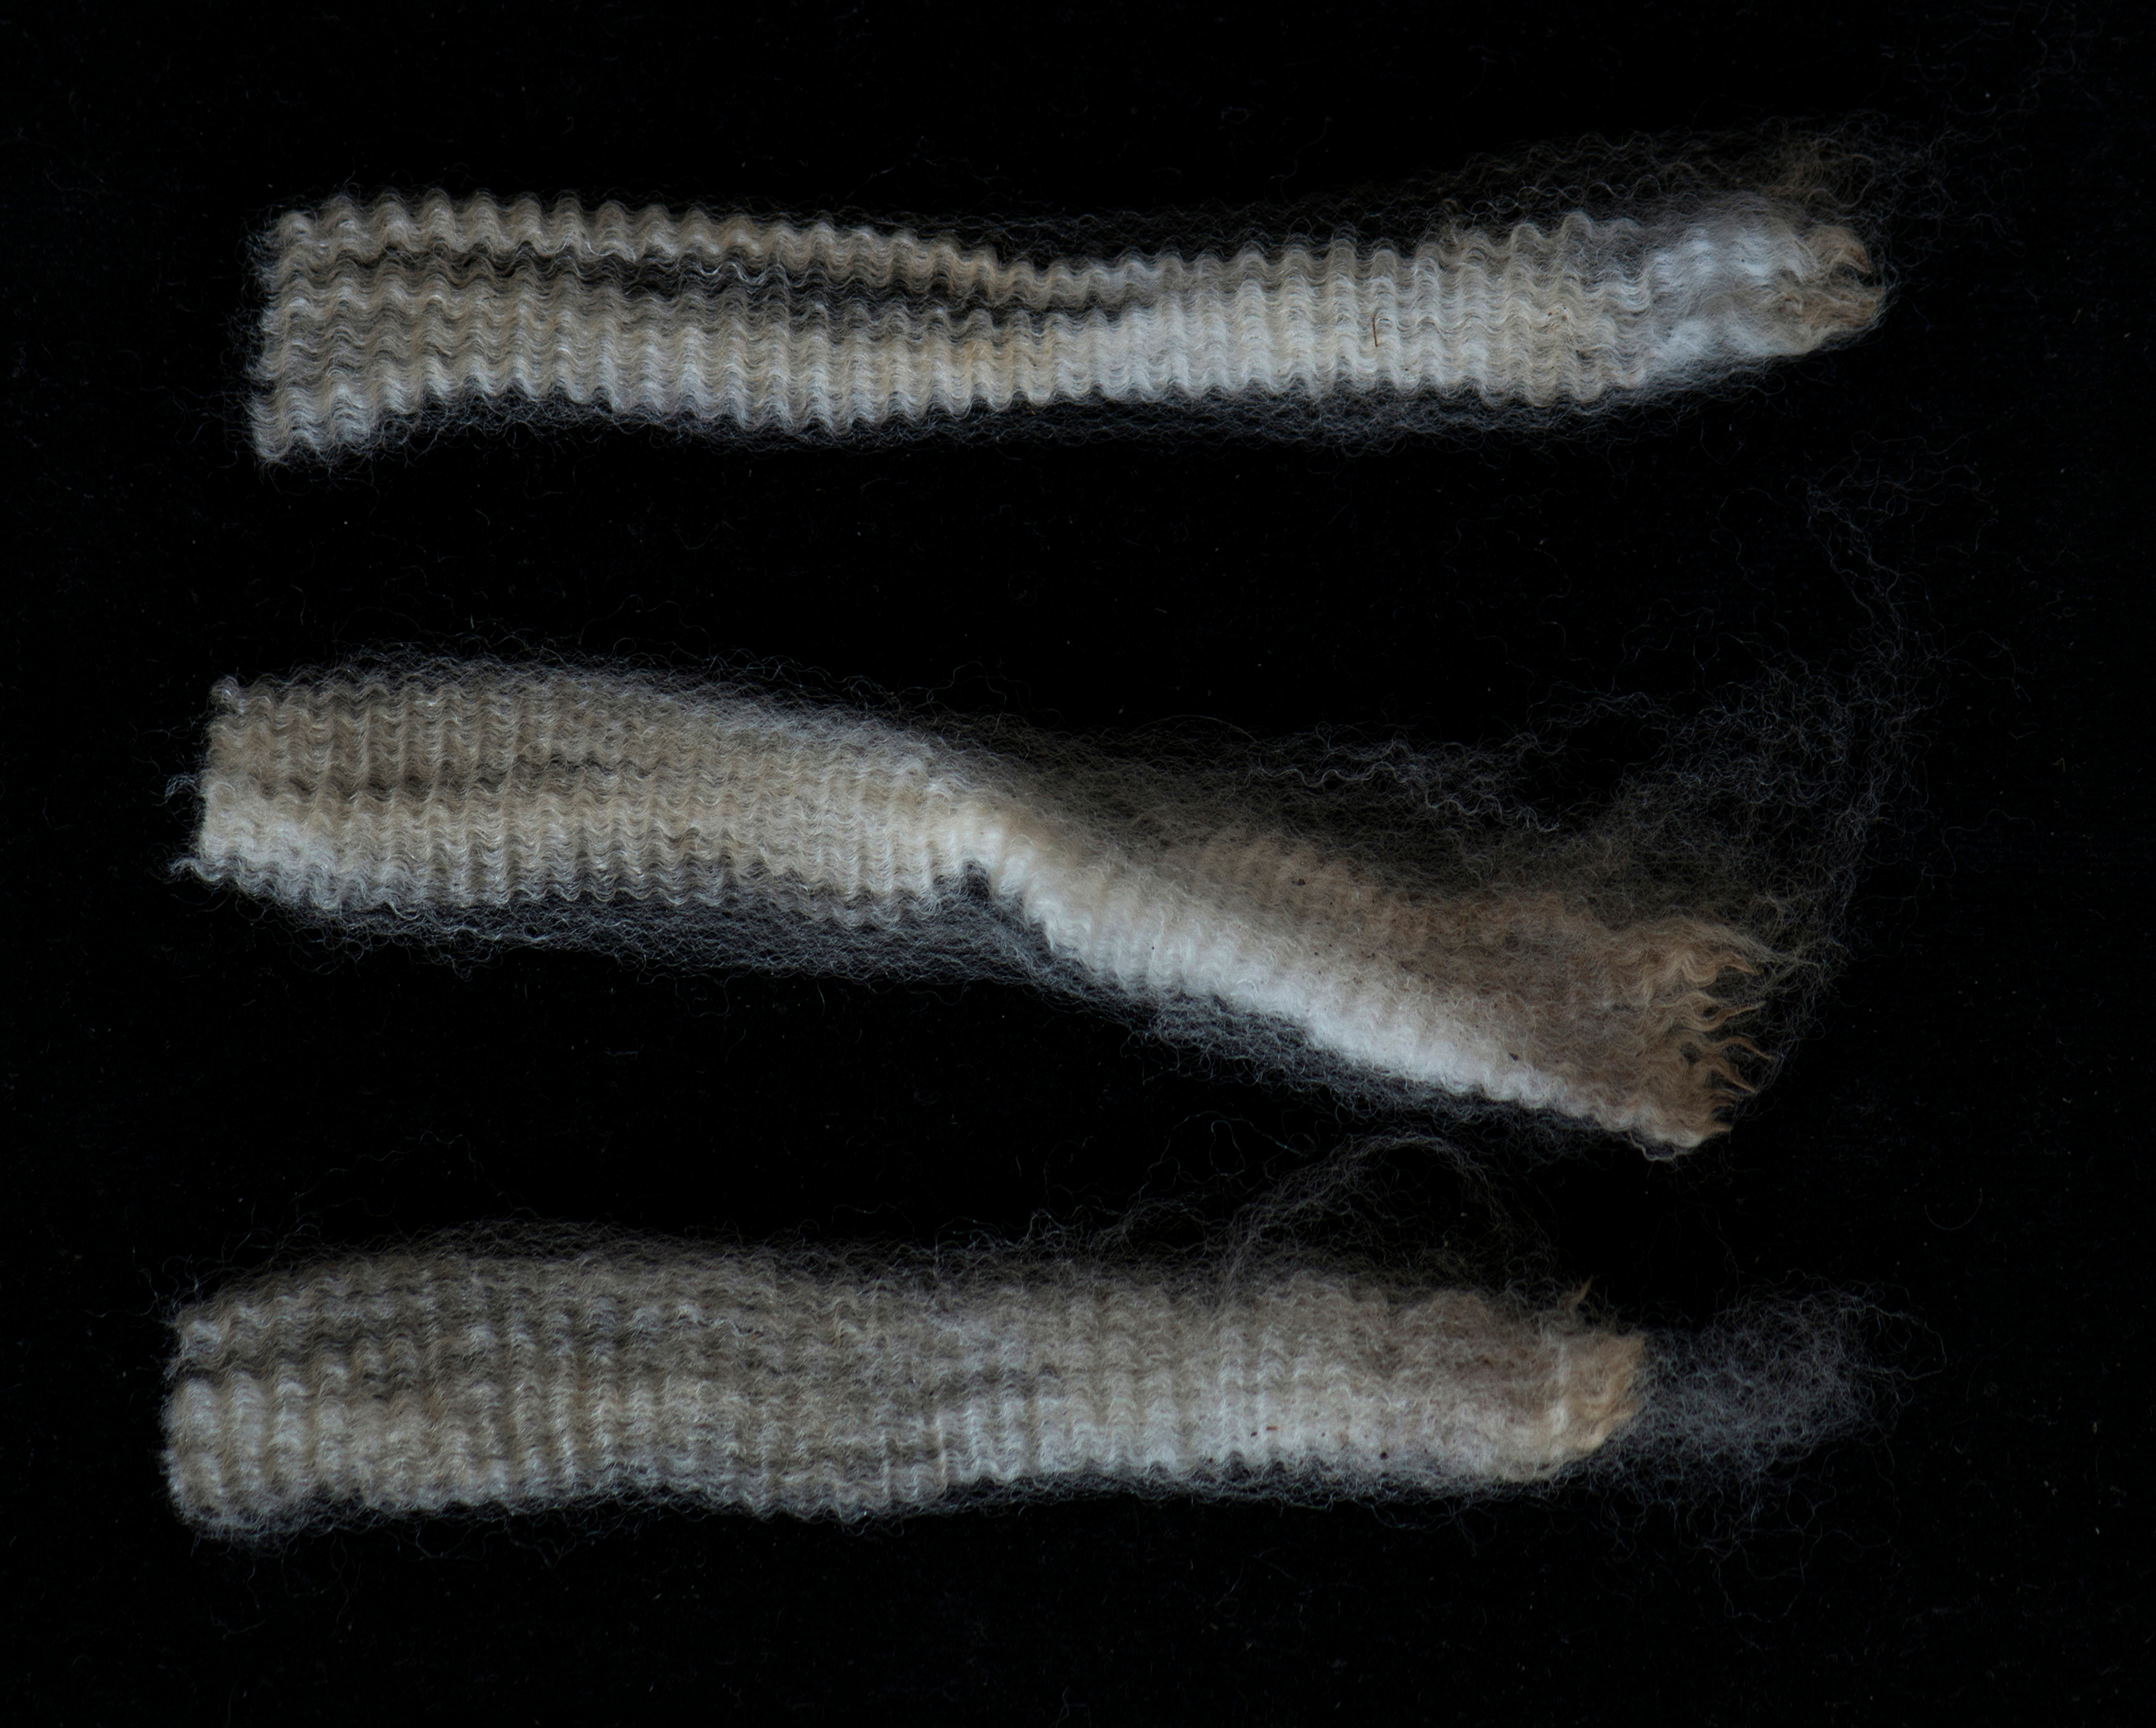
\includegraphics[width=1.0\textwidth,angle=180]{figwoolphoto.jpg}
  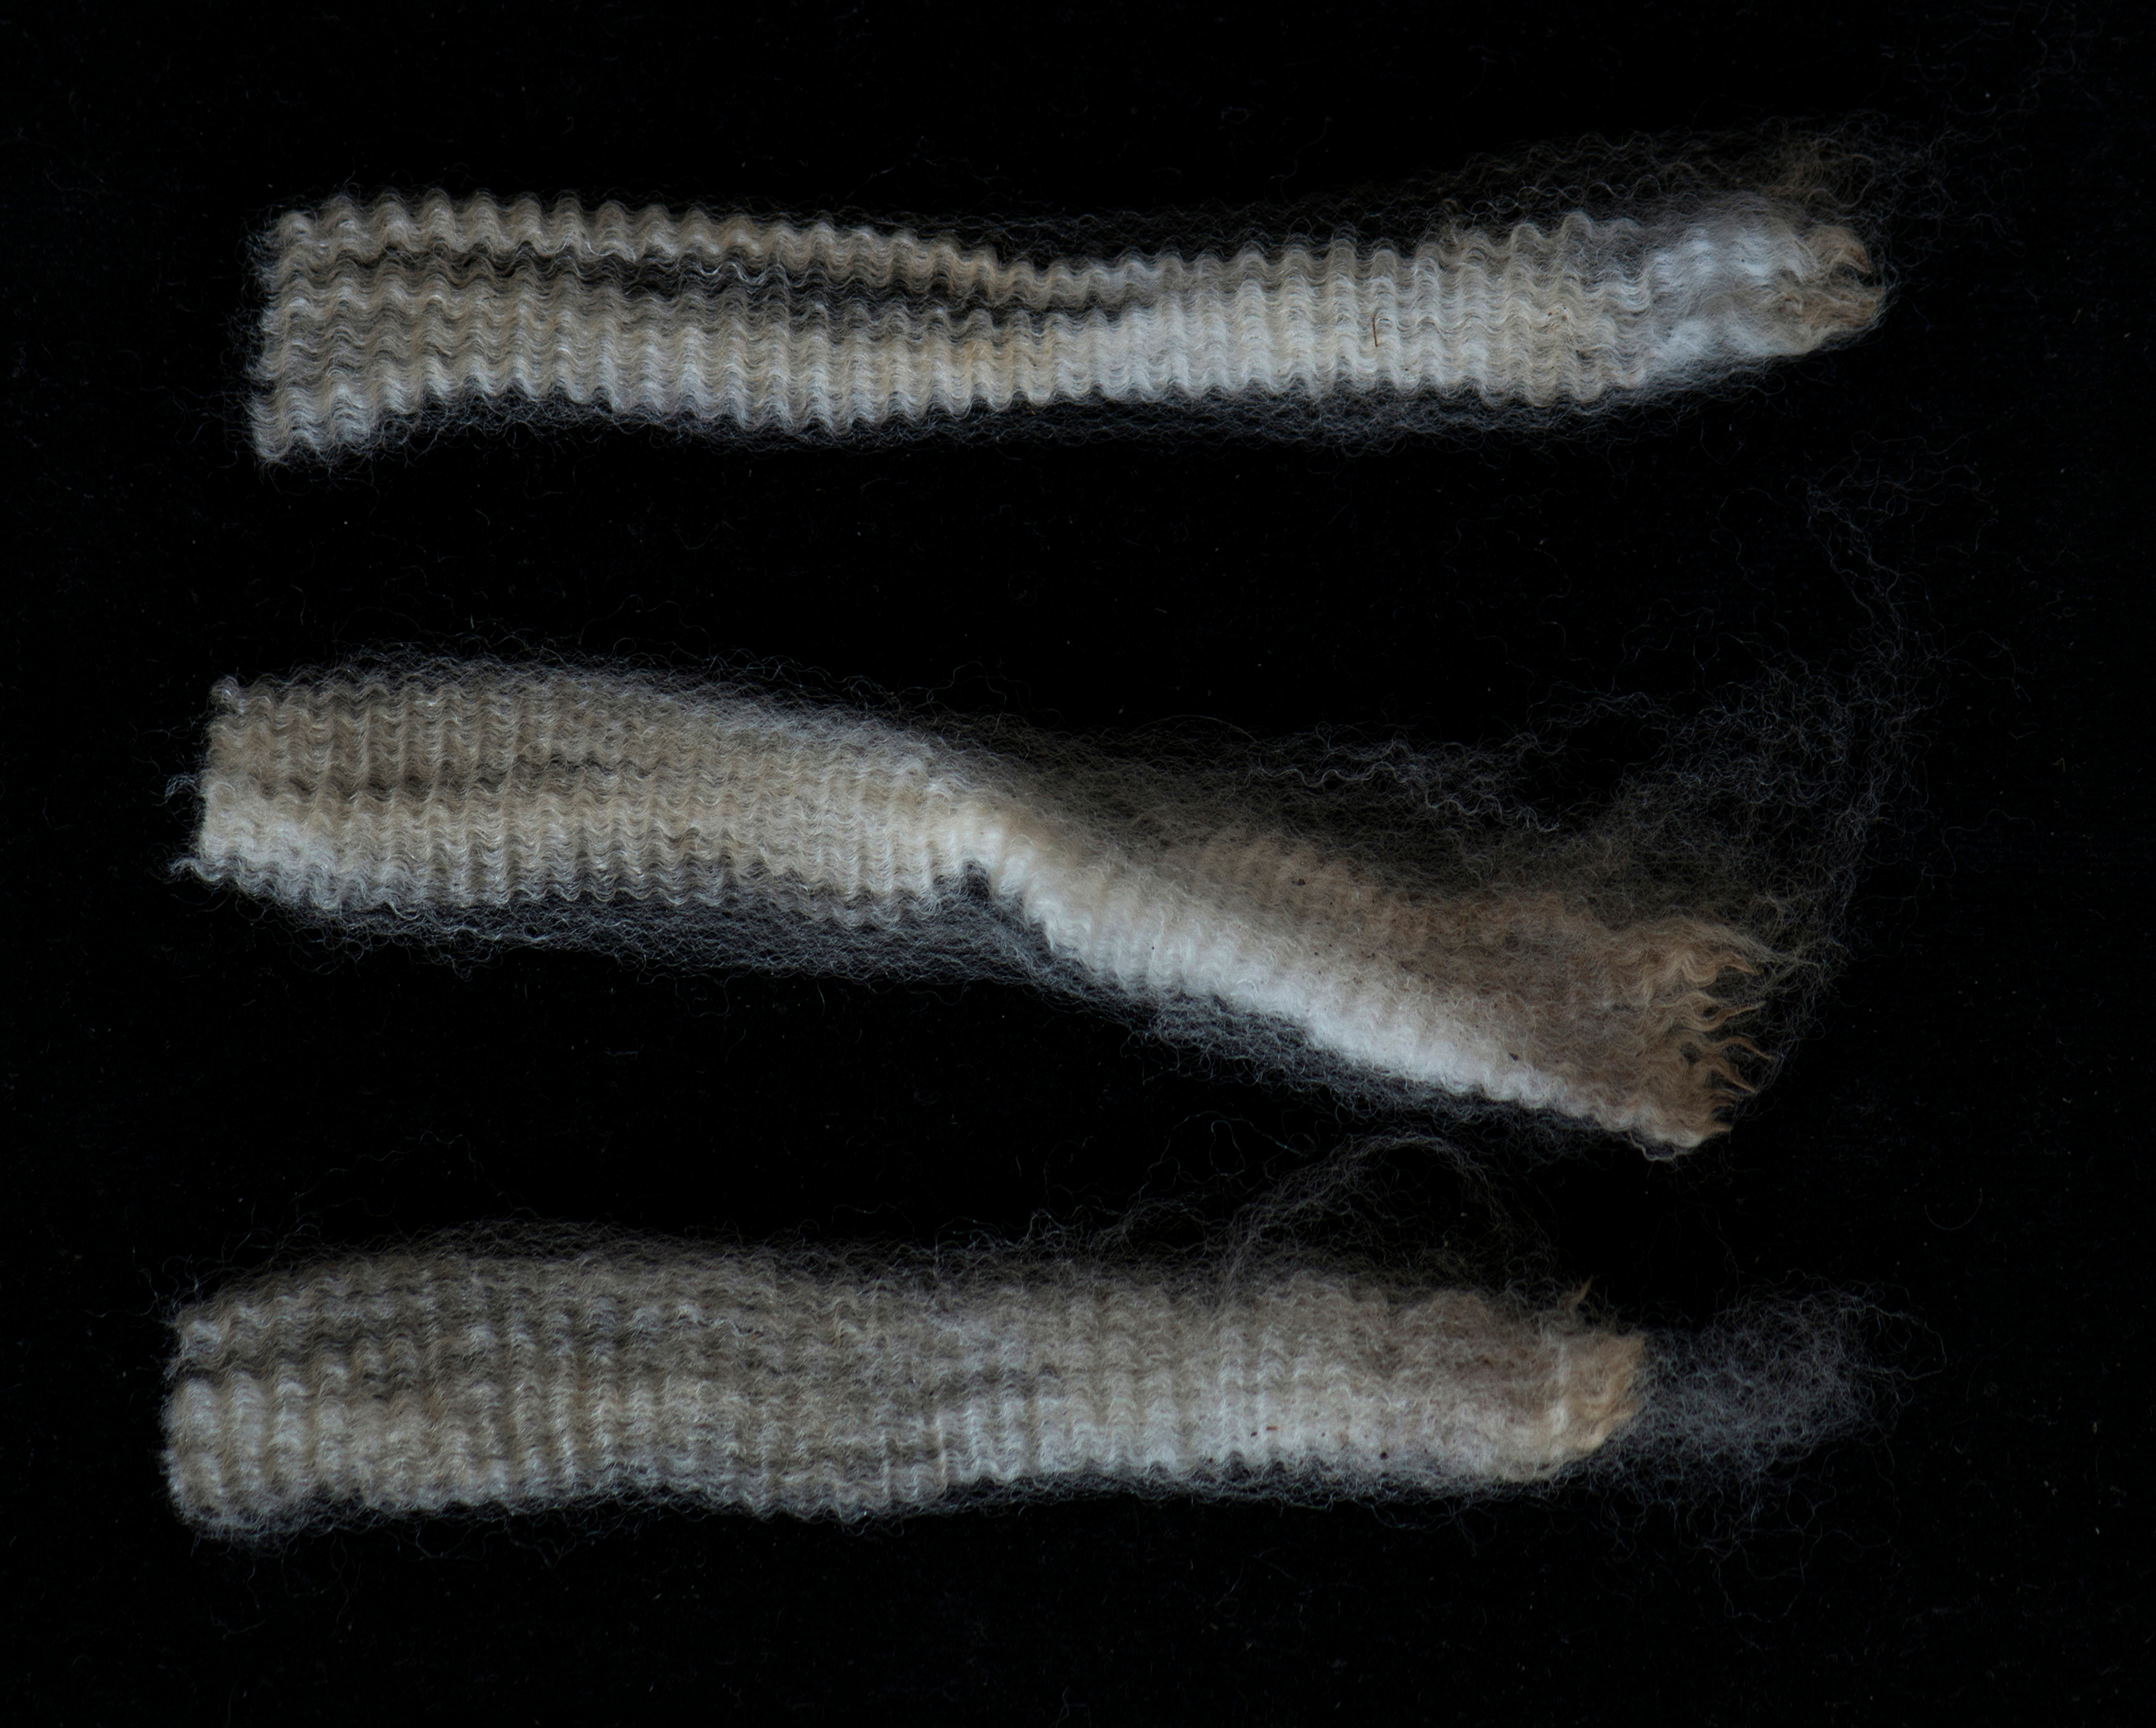
\includegraphics[scale=0.52]{figwoolphoto.jpg}
%   photo549.499.525.jpg is original photo 
  \caption{Photograph showing a three Merino wool staples representing (top to bottom) the {\em unfolded}, {\em stretched}, and {\em unaligned} staple crimp types. }
  \label{fig:woolphoto}
\end{figure}

%\end{document}


%\documentclass{article}
%\usepackage{graphicx}
%\usepackage{caption,rotating}
%\usepackage{subfigure}
%\begin{document}
\begin{figure}
\begin{turn}{90}
\begin{minipage}[c][\textwidth][c]{\textheight}
 \subfigure[Unaligned staple crimp type]{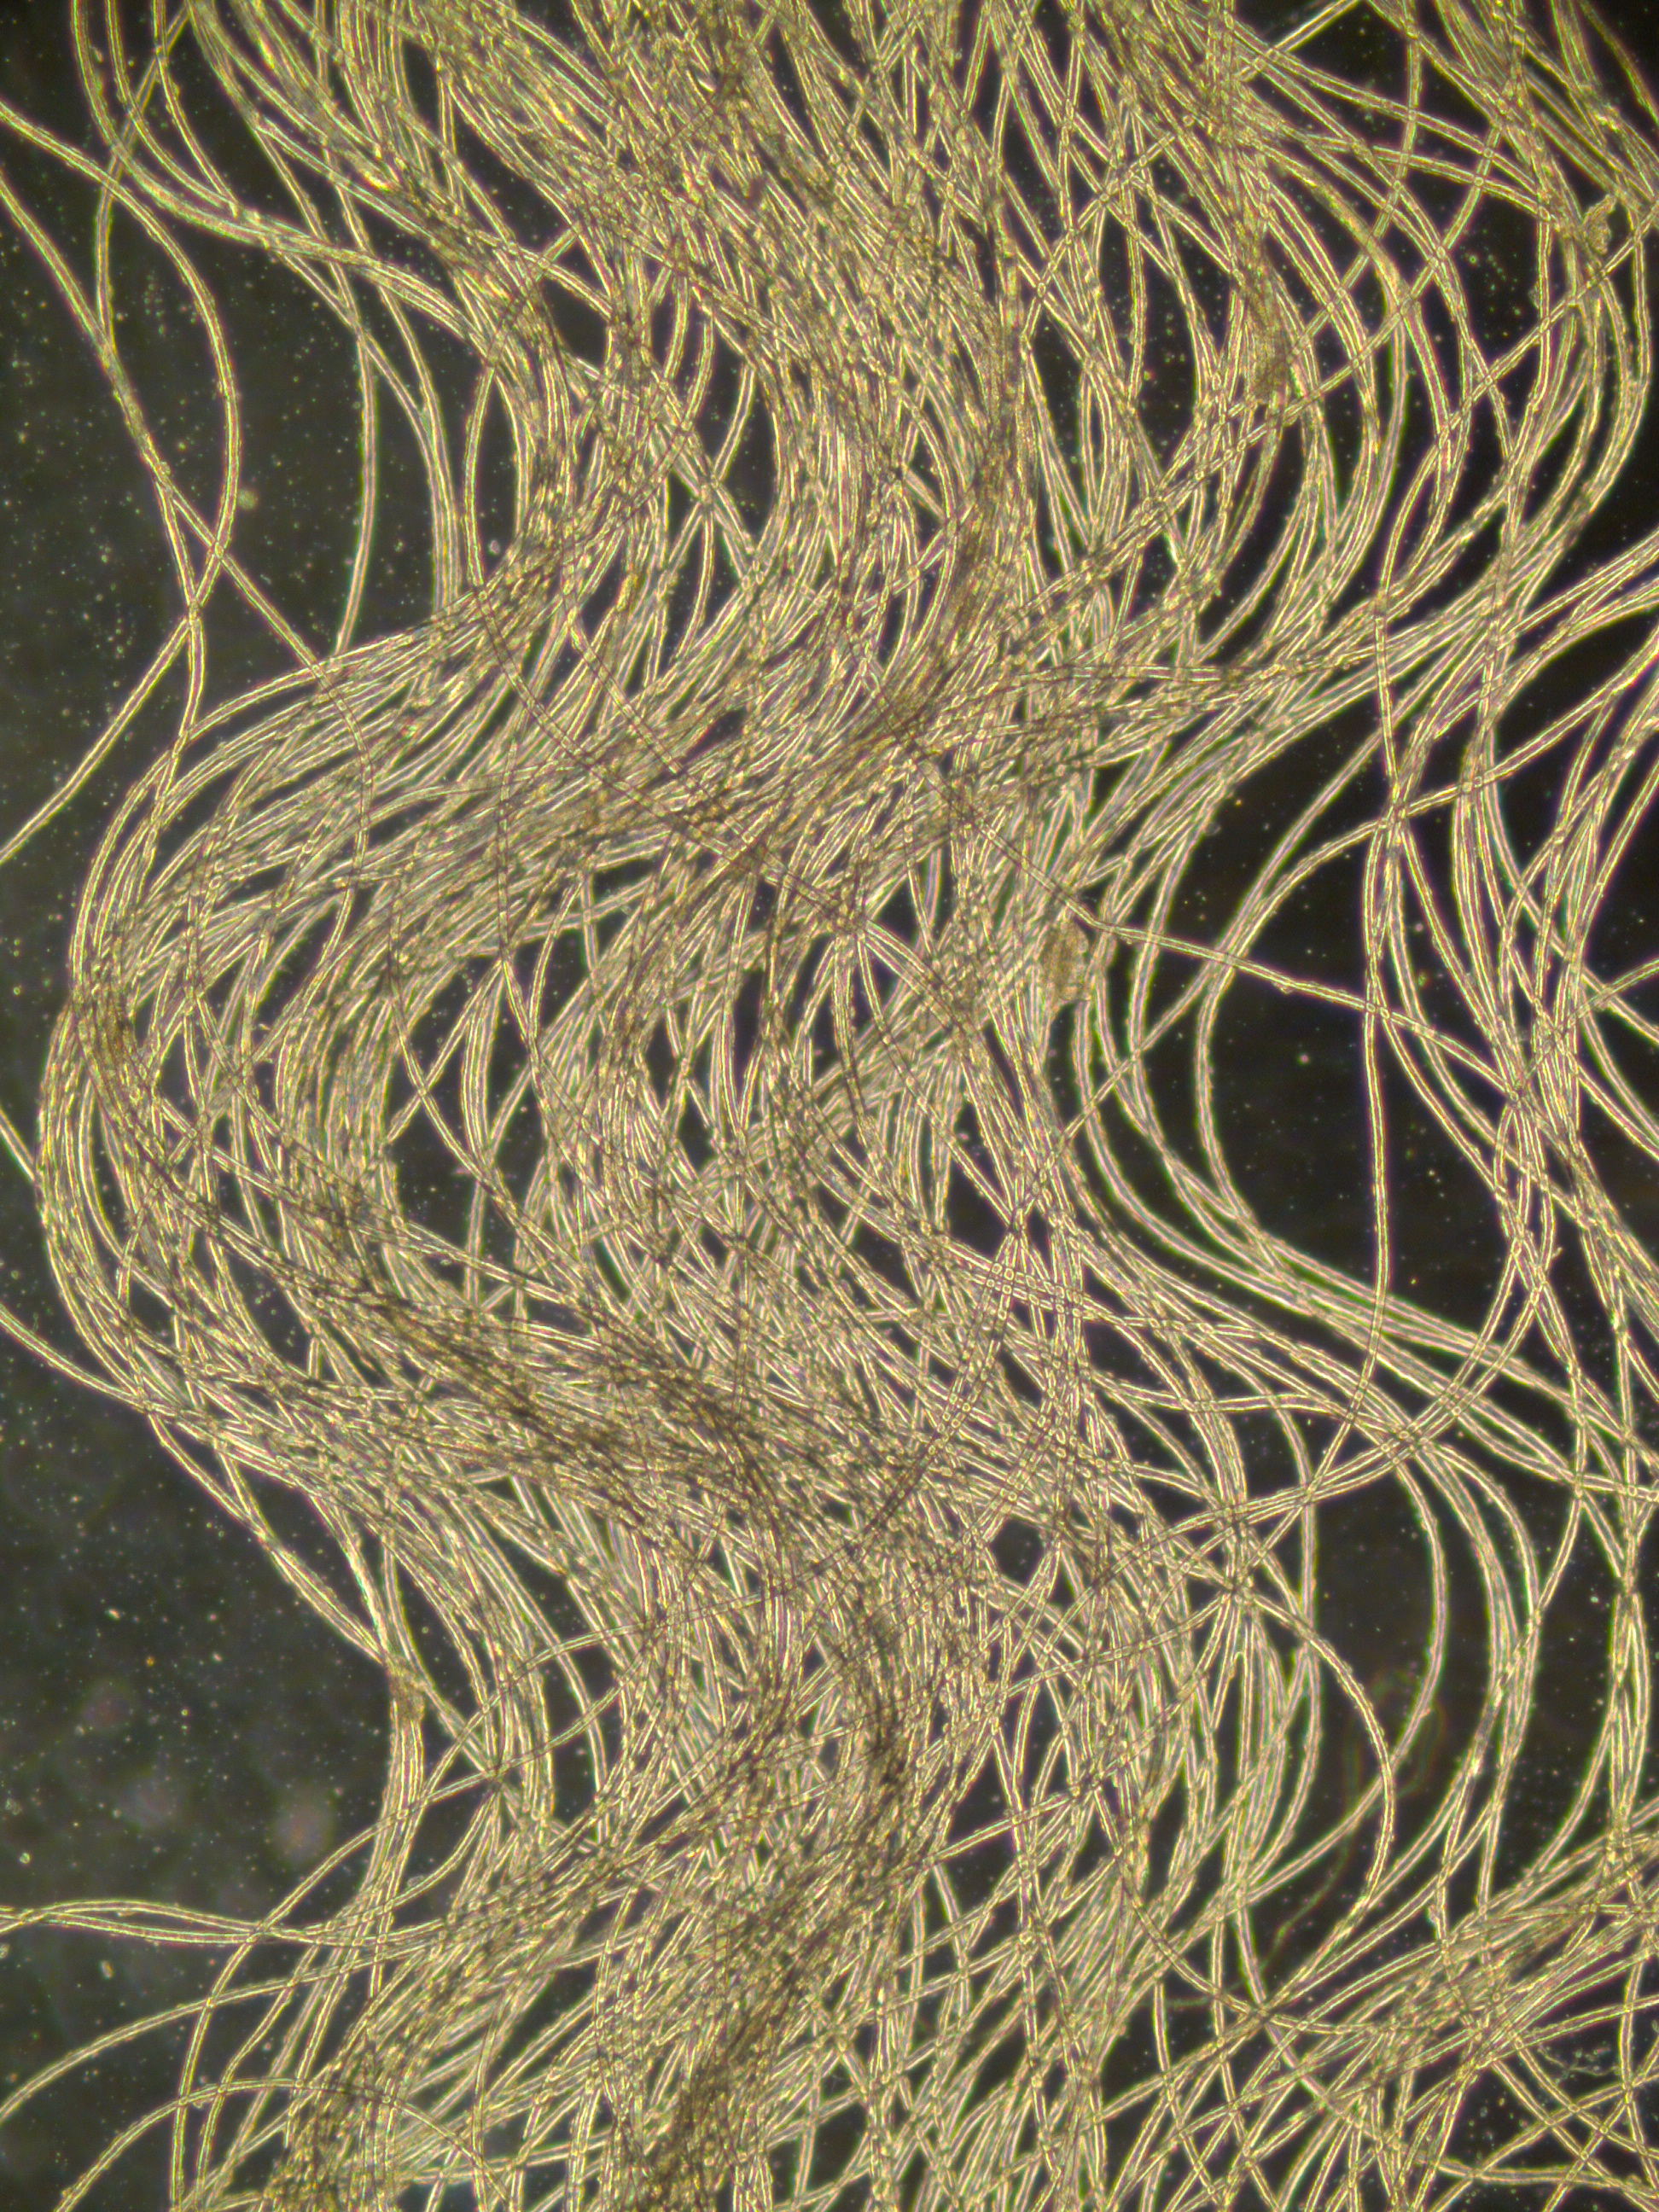
\includegraphics[scale=0.38]{figfibresunalignedrot.jpg}}\hfill
 \subfigure[Stretched staple crimp type]{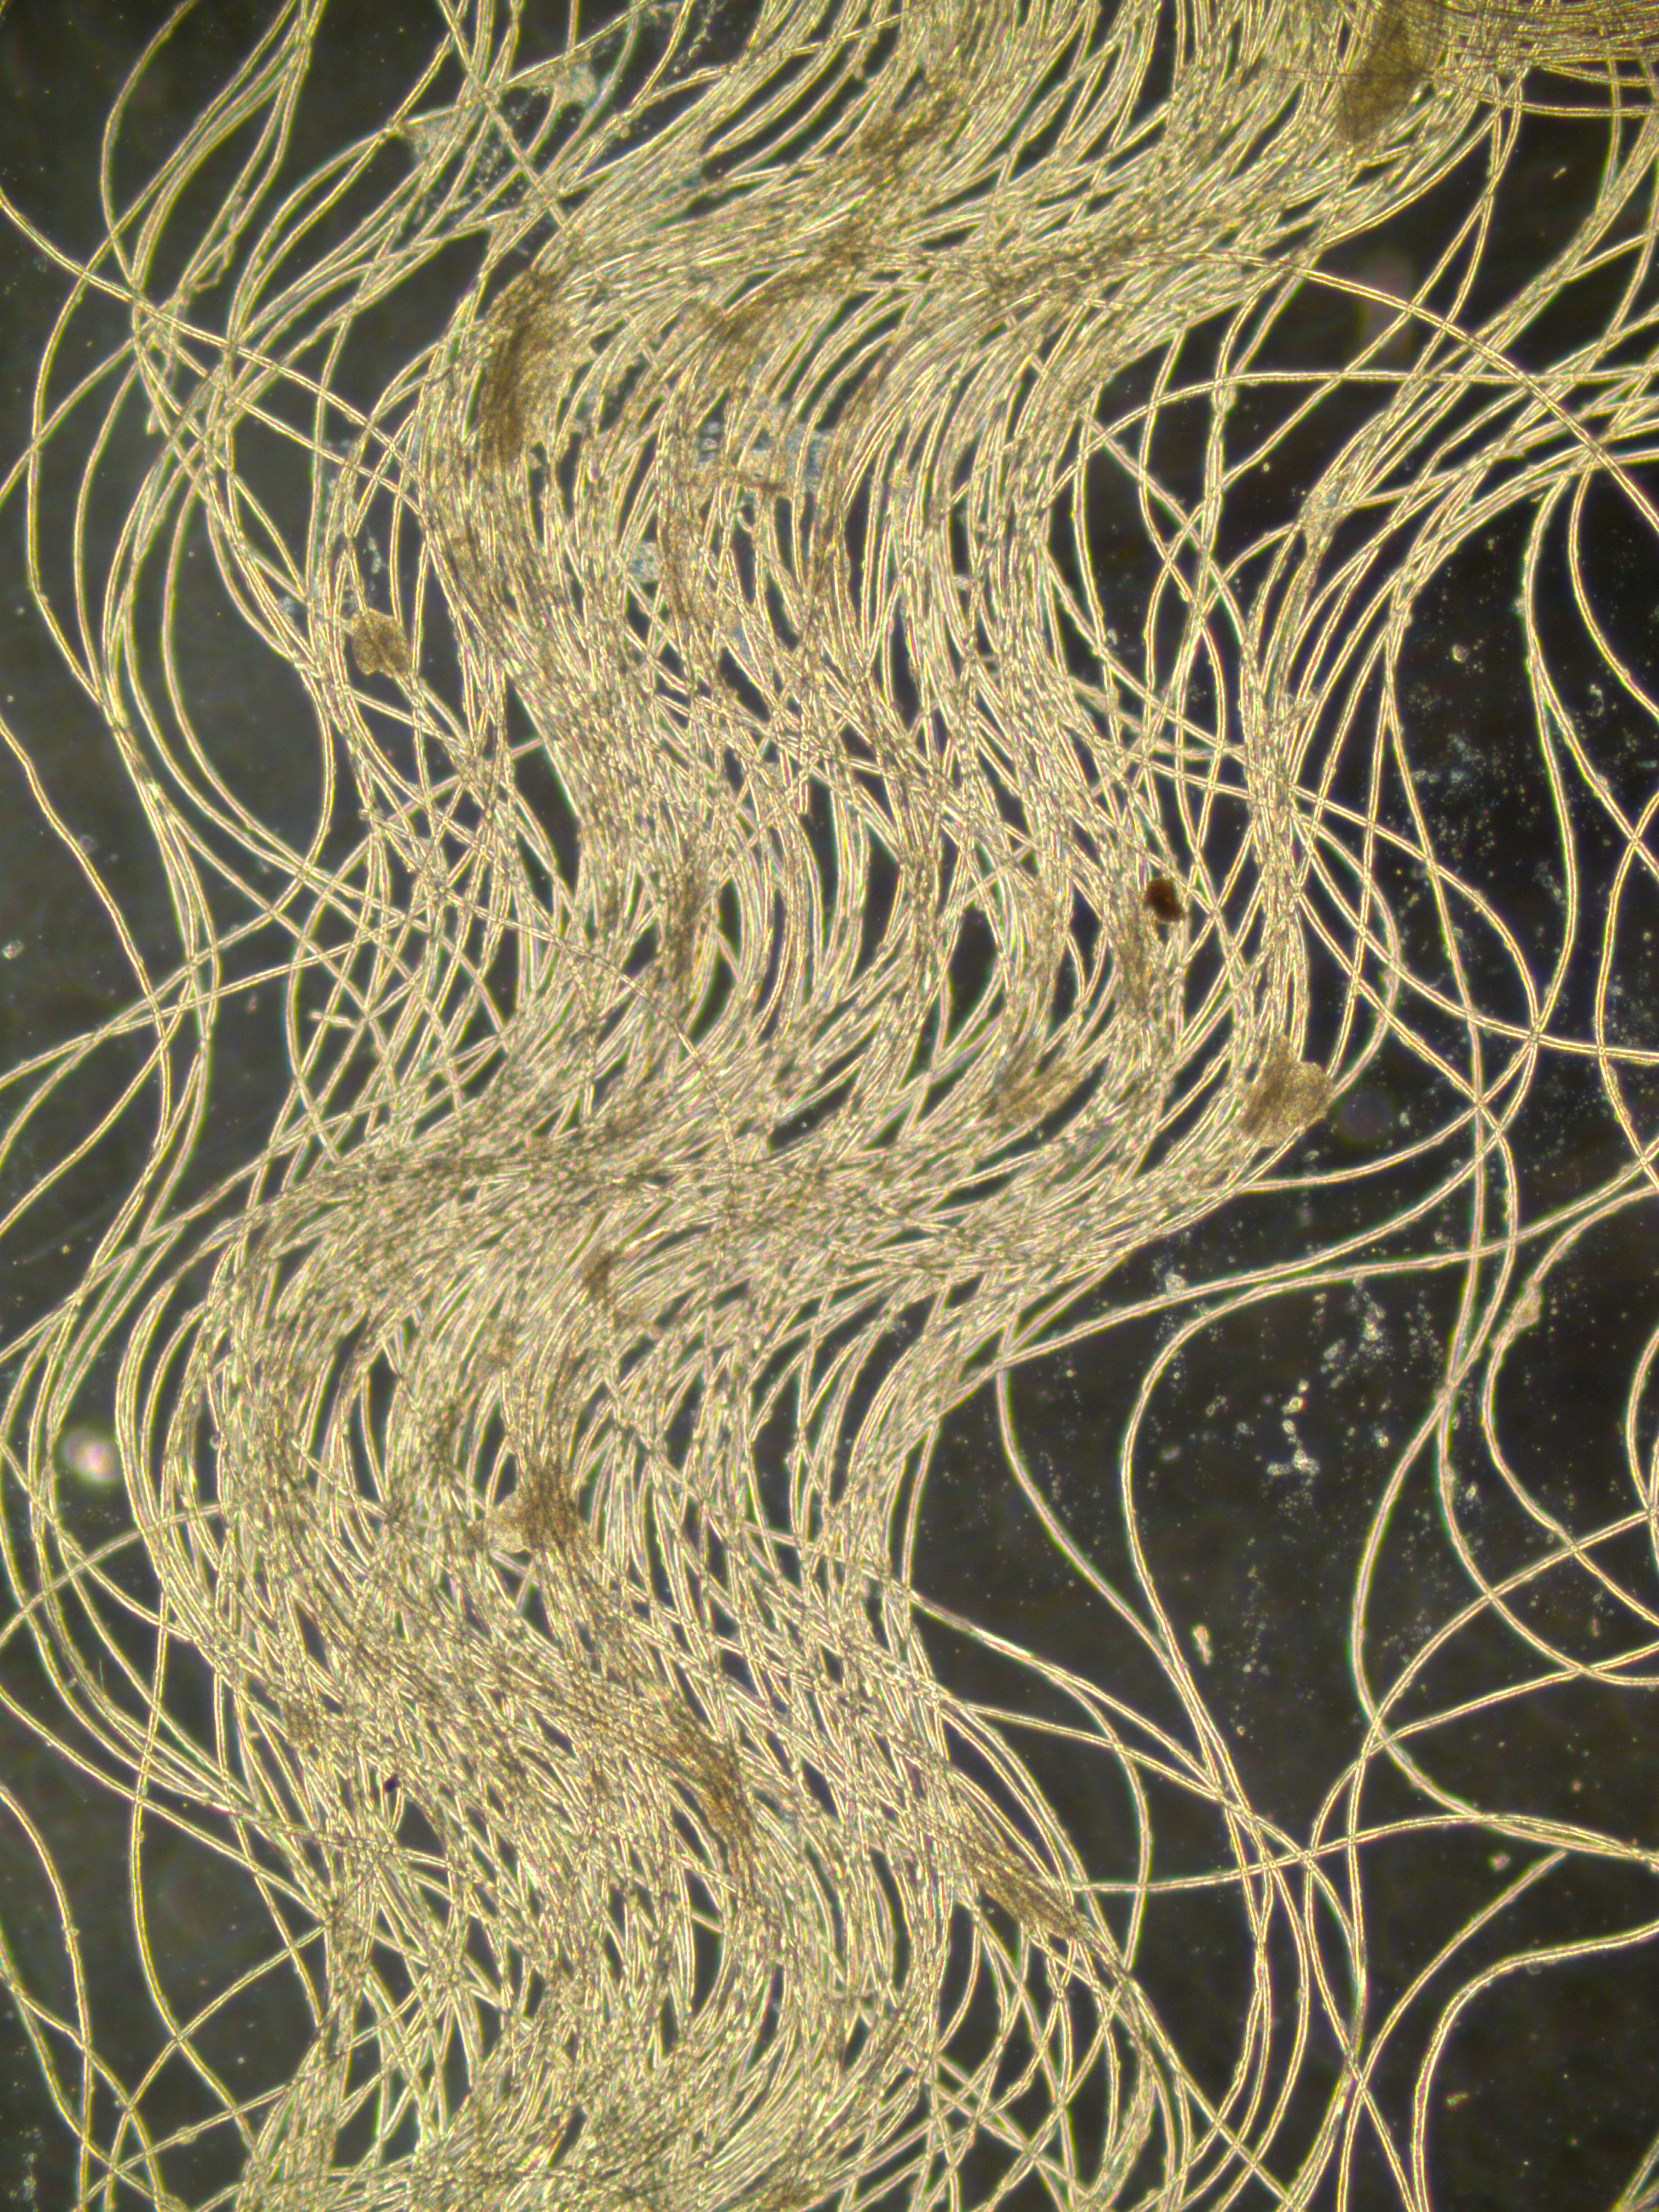
\includegraphics[scale=0.38]{figfibresstretchedrot.jpg}}\hfill
 \subfigure[Unfolded staple crimp type]{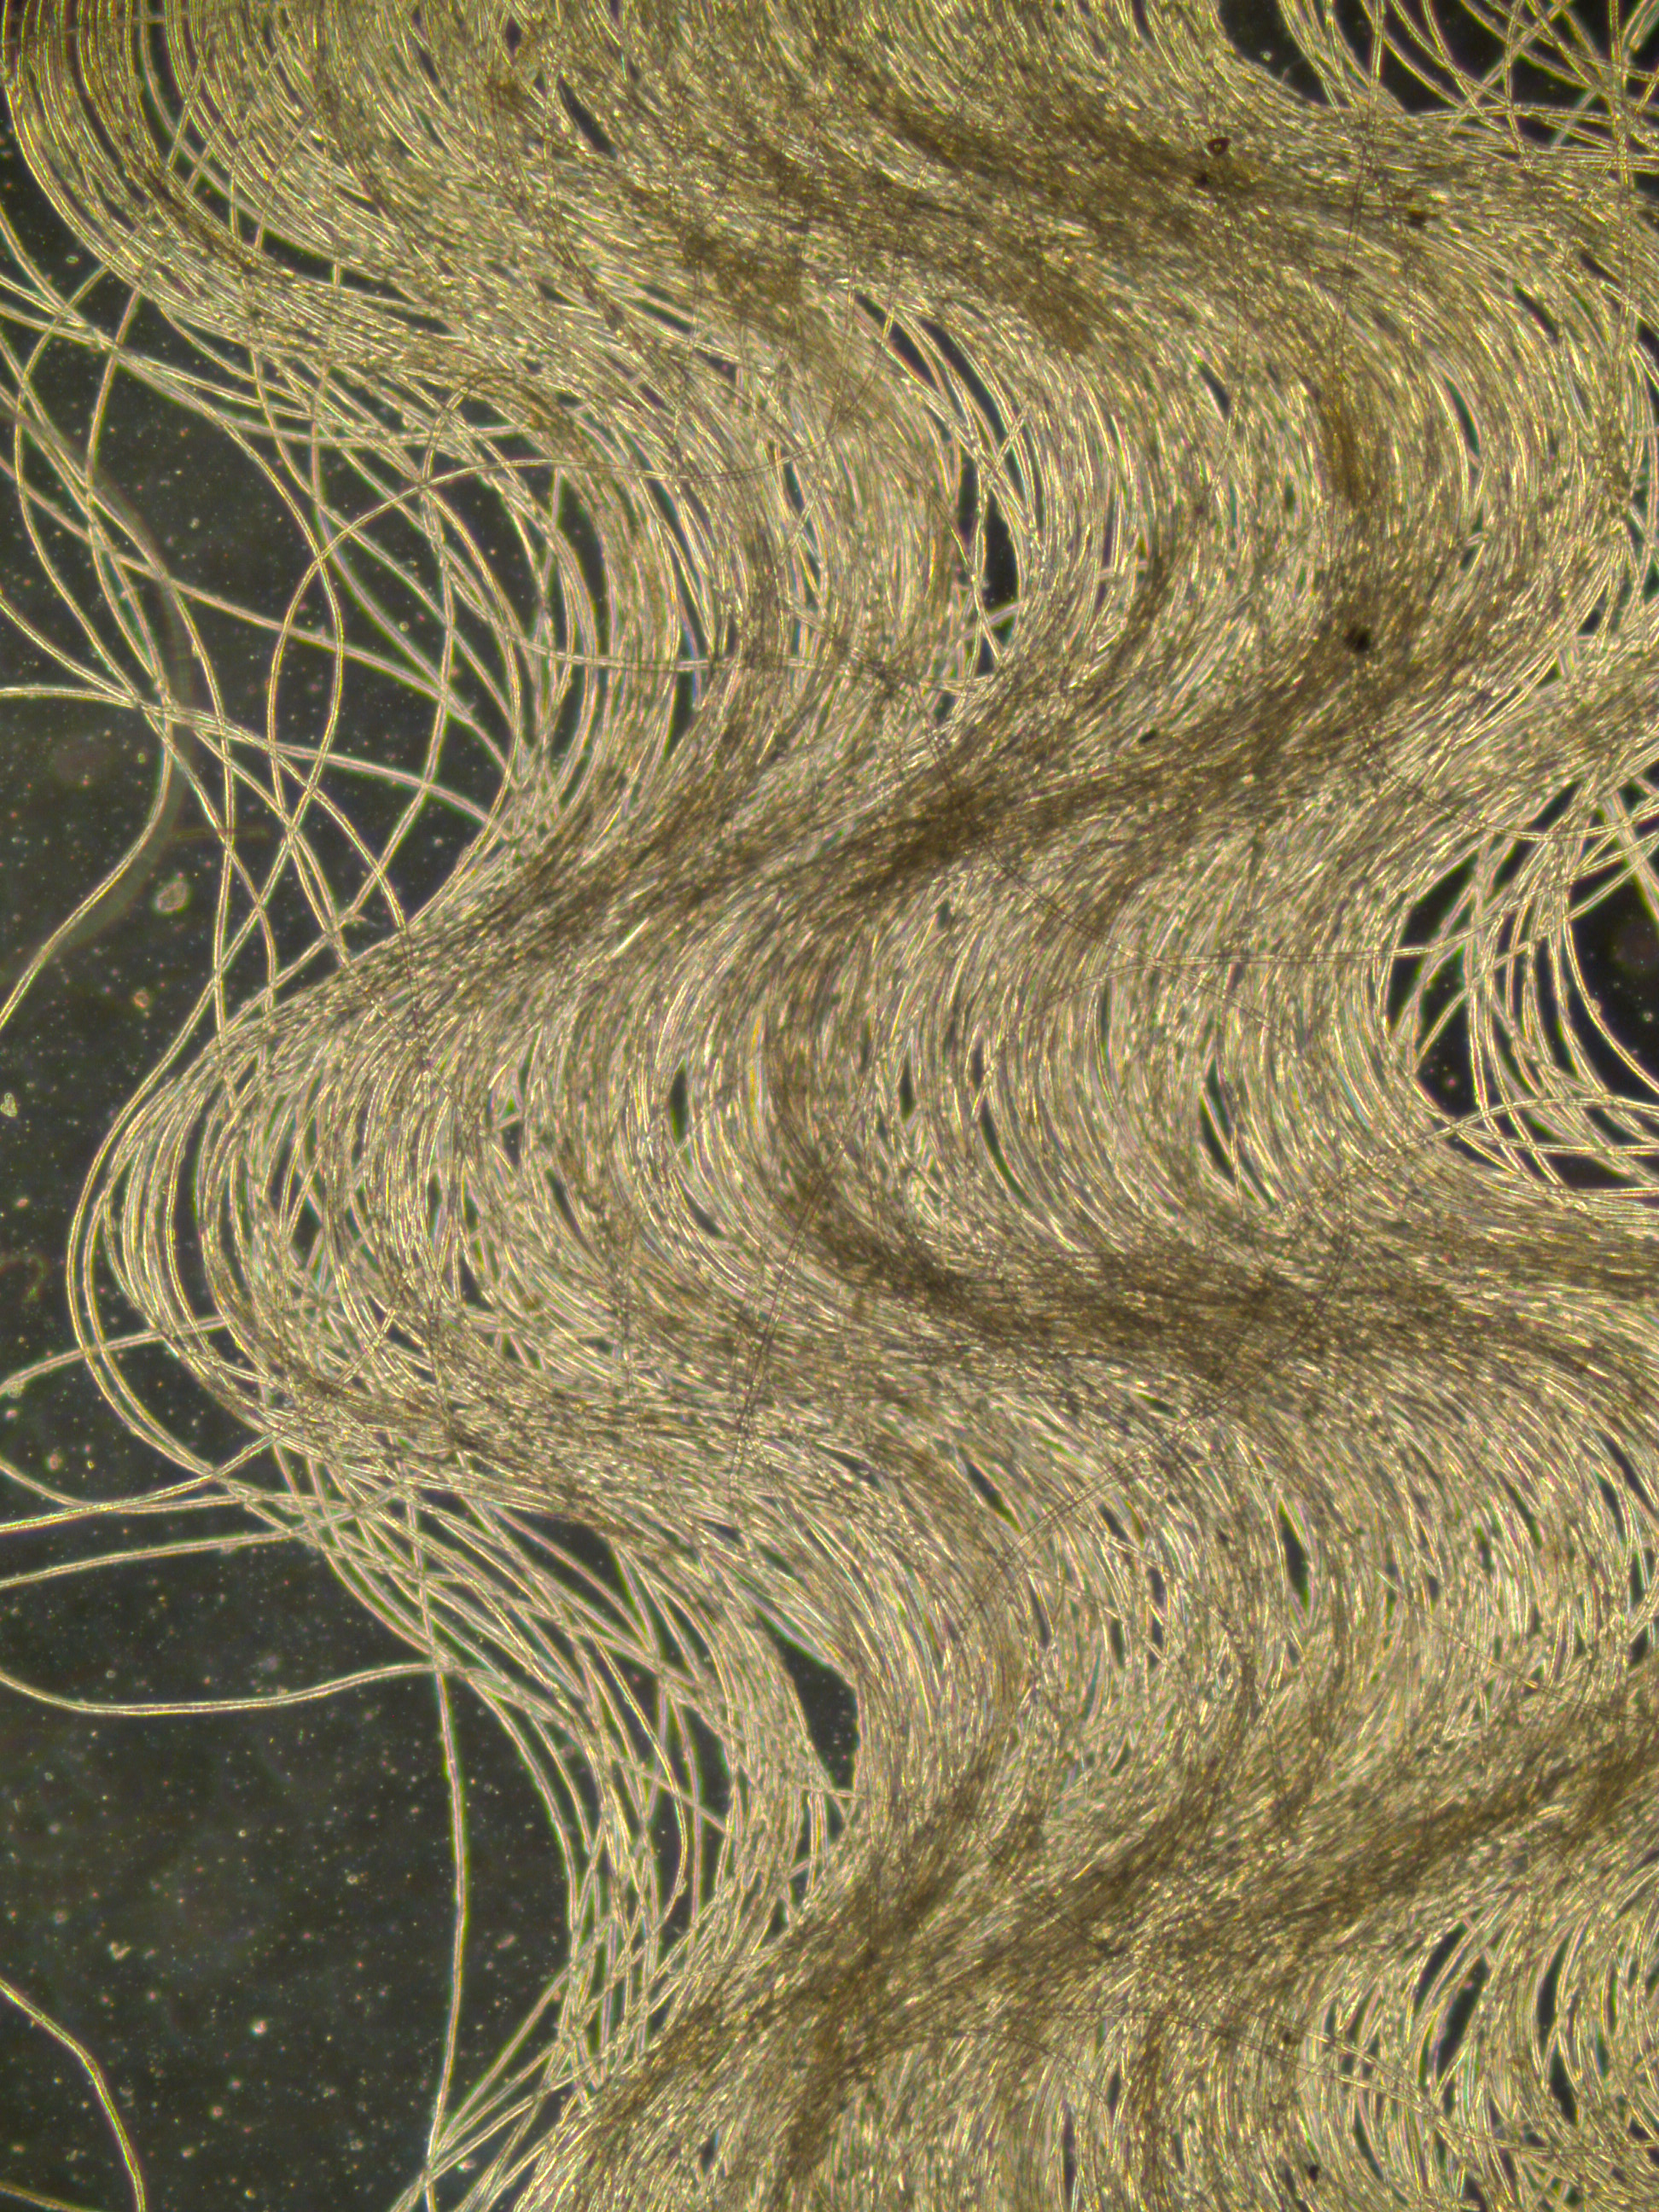
\includegraphics[scale=0.38]{figfibresunfoldedrot.jpg}}
\caption{Photomicrographs, taken with phase contrast microscope, showing multi
ple bundles of fibres for each of the three staple crimp types. Microscope magnification 25x. For printed magnification see Appendiox A.}
\label{fig:fibre3types}
\end{minipage}
\end{turn}
\end{figure}
%\end{document}

The increase in fibre alignment from unaligned to stretched to unfolded is obvious in  Figure~\ref{fig:fibre3types} . This is in line with our statement that fibre alignment is important in determining whether a wool will have a stretched helix or an unfolded helix crimp.

In defining these three types we do not mean to imply that they form some sort of continuous scale. There is a gradation from {\em unaligned} to {\em stretched} , but the step from {\em stretched} to {\em unfolded} is a quantum leap. A fibre bundle has to be either stretched or unfolded, it cannot be both or half way between. A sheep may be a mosaic with some fibre bundles stretched, and others unfolded. A staple may contain a mix of stretched and unfolded bundles - some traditional superfine Merino wools exhibit this. A single bundle must be one or the other.

Given these definitions, we can classify wools according to the above three staple crimp types and examine data on their defining properties.

The first thing to examine is the prediction that in wools with an unfolded helix crimp the fibres in a bundle will be close together at the points of twist, and spaced apart at the peaks and troughs. This is easier to see in the single fibre bundle shown in Figure~\ref{fig:twist} than in the multiple bundles shown in  Figure~\ref{fig:fibre3types}, but it is there in both and is a nice confirmation of our suggested mechanism for unfolding.

The next thing to note is that fibre alignment is part of our definition of the three types of staple crimp. We cannot therefore use staples graded in this way to determine the importance of alignment. We consider alignment to be so important that we have made it part of the definition. We can, however, look at the factors which might affect alignment. One of these might be variation in the length growth rate of fibres. We measure this as the standard deviation of fibre length. Figure~\ref{fig:sdlfbox} shows a boxplot of the standard deviation of fibre length for a number of sheep representing each of the three crimp types. The {\em unaligned} type clearly has a higher standard deviation of fibre length, but the other two types do not differ. The heavy bars in the boxplot show the median values. The means are 11.8, 17.2, and 12.5 for stretched, unaligned and unfolded respectively. The respective standard errors are 1.82, 1.68, 1.48 so the unaligned group is significantly different from the other two. An almost identical result is obtained if we use coefficient of variation of fibre length instead of standard deviation of fibre length.

%\documentclass{article}
%\usepackage{graphicx,subfigure}
%\begin{document}

\begin{figure}[!h]
  \centering
  \includegraphics[width=1.1\textwidth]{figsdlfbox.png}
%   sdlfbox.png is original 
  \caption{Boxplot showing the standard deviation of fibre length for wools graded as {\em unaligned}, {\em stretched} and {\em unfolded} crimp types. Data from one Merino flock with 7,6, an d 9 sheep respectively representing each type}
  \label{fig:sdlfbox}
\end{figure}

%\end{document}



It is worth looking a little closer at the distribution of fibre lengths to see how the unaligned crimp type differs from the others. Figure~\ref{fig:minlfbox} shows a boxplot of minumum fibre length for the same sheep as in Figure~\ref{fig:sdlfbox}. It is clear that the unaligned crimp type has a much lower minimum fibre length and therefore a greater proportion of short fibres. 

%\documentclass{article}
%\usepackage{graphicx,subfigure}
%\begin{document}

\begin{figure}[!h]
  \centering
  \includegraphics[width=1.1\textwidth]{figminlfbox.png}
%   minlfbox.png is original 
  \caption{Boxplot showing the minimum  fibre length for wools graded as {\em unaligned}, {\em stretched} and {\em unfolded} crimp types. Data from one Merino flock with 7,6, an d 9 sheep respectively representing each type}
  \label{fig:minlfbox}
\end{figure}

%\end{document}


 
So it is clear that uneven fibre lengths contribute to poor fibre alignment, but not to the difference between well-aligned-stretched crimp and unfolded crimp. At least not in these data. So maybe our ideas about even fibre length being important for unfolding to occur are not correct? It may be just as important for a well formed stretched helix crimp. Perhaps  it would be better to say that it is not possible to form an unfolded crimp when the fibre lengths are uneven.

It is easy to see how uneven fibre lengths will affect alignment. If some fibres grow slower than others, they will either stay at the staple tip and their crimp will be more stretched pulling them out to a smaller amplitude than the  other fibres, or they will pull back from the staple tip resulting in a staple with a pointed tip , an uneven crimp at the tip end, and an out of phase crimp elsewhere. The former seems to happen in Merino sheep, the latter in British breeds and their crosses.

Uneven fibre lengths is not the only factor affecting fibre alignment. We list all the factors which may affect alignment as follows
\begin{itemize}
\item Standard deviation of fibre length. See above
\item Standard deviation of radius of curvature. If the curvature varies from fibre to fibre, then obviously their crimps will be out of phase
\item Variation in the orientation of the plane of curvature. Fibre emerge from a follicle curved in one direction. If those directions vary from fibre to fibre, the crimp waves will not all be in the same plane, and will appear to be out of alignment even if the frequencies and amplitudes are the same
\item Lustre seems to be associated with well aligned fibres. We do not know why. It may be a consequence, rather than a cause of alignment. That is aligned fibres may simply appear more lustrous.
\item Shedding of fibres will obviously lead to poor alignment because fibres move and felt if not secured in a follicle
\end{itemize}


We should realize that well aligned fibres is only part of the set of conditions which determine whether stretching or unfolding occurs. The other very important factor is the spatial arrangement of follicles in the skin and the consequent spatial arrangement of fibre contacts in the growing fleece. To this end we studied the spatial distribution of follicle density in the same sheep used for the fibre length and alignment investigation above.


We chose one sheep representing each of the unaligned, stretched, and unfolded crimp types. On a horizontal skin section under the projection microscope we oriented the specimen so that the rows of follicle groups ran across the image, so that the direction referred to as {\em north} in Section~\ref{sec:further} is at the top of the image. This orientation was readily achieved by placing the side of the follicle groups occupied by the 3 primary follicles and their sweat glands at the top of the image. The precise positioning of {\em north} was the sweat gland duct of the central primary follicle. One follicle group was chosen at random and we measured the distance between the perimeter of the chosen group and the contact point of its nearest neighbour in the north, south, east, and west directions. These data are shown in Table~\ref{tab:igdist}

%\documentclass{article}
%\usepackage{lscape}
%\begin{document}

\begin{table}[htp]
\centering
\caption{Intergroup distances for one sheep representing each of the unaligned, stretched, and unfolded crimp types}
\label{tab:igdist}
\vspace{0.1in}
\begin{tabular}{|p{0.7in}|p{0.6in}|p{0.6in}|p{0.6in}|p{0.6in}|}  \hline
     Crimp Type & North neighbour & East neighbour & South neighbour  & West neighbour  \\ 
   & microns  & microns & microns & microns \\ \hline
 Unfolded & 184 & 96 & 136 & 72 \\
 Stretched & 48 & 60 & 52 & 32  \\
 Unaligned & 44 & 60 & 56 & 40 \\ \hline
\end{tabular}
\end{table}

%\end{document}


The differences are quite clear. In the sheep of unfolded crimp type the follicle groups were spaced further apart, particularly in the north and south dirctions, but also in the east and west directions. This result helps confirm our idea that unfolding of fibre bundles requires space between the bundles. This space is provided by the spacing of the follicle groups, because a fibre bundle corresponds to a follicle group.

One might ask then, if sheep with an unfolded crimp type have more space, how can they have a high density? The answer is that the space between follicles within a follicle group is considerably reduced.  This is shown in Table~\ref{tab:ifdist}

%\documentclass{article}
%\usepackage{lscape}
%\begin{document}

\begin{table}[htp]
\centering
\caption{Interfollicular distances within a follicle group for one sheep representing each of the unaligned, stretched, and unfolded crimp types}
\label{tab:ifdist}
\vspace{0.1in}
\begin{tabular}{|p{0.7in}|p{0.4in}|p{0.4in}|p{0.4in}|p{0.4in}|p{0.4in}||p{0.4in}|} \hline
     Crimp Type & Site 1 & Site 2 & Site 3 & Site 4 & Site 5 & Median\\ 
   & microns  & microns & microns & microns  & microns\ & microns\\ \hline
 Unfolded & 12 & 12 & 5 & 8  & 12 & 12 \\
 Stretched & 20 & 16 & 20 & 28 & 20 & 20 \\
 Unaligned & 36 & 24 & 32 & 36 & 40 & 36 \\ \hline
\end{tabular}
\end{table}

%\end{document}

 
There is a  gradation in interfollicular distances within a follicle group from unaligned to stretched to unfolded. The closer follicles in the unfolded case will obviously compensate for there being a greater space between follicle groups, so that the overall follicle or fibre density will not be reduced, and will probably exceed that of the other types. An important side effect of the high within group follicle density in sheep of the unfolded crimp type, is that the fibre diameter will be considerably finer. 

We have to concede that we have not been able to confirm all of the predictions concerning differences between unfolded helix wools and stretched helix wools made in Section~\ref{sec:further}. We have confirmed that uniformity of fibre length and spatial distribution of follicle groups are important, but there may be other factors. We have addressed the question of fibre alignment, but because it is built into our definition of the three crimp types we cannot clarify whether it is a cause or an effect in the question of whether a particular sheep will have a stretched or unfolded crimp type.

\subsection{Staple formation}
The factors which we have identified as affecting the crimp in a staple may also affect the overall form and size of staples. When we look at a fleece we see both the crimp and the staple form simultaneously. So we should be able to use both crimp and staple form to infer something about the underlying causal factors, which may themselves be difficult to observe or measure.

After a sheep is shorn, the crimp is visible almost immediately the wool starts to regrow, but the staples do not start to separate until about 25mm of fleece is grown. The crimp therefore precedes the staple formation, and cannot be caused by it, although, as noted above , there may be common causes.

One aspect of staple formation which is known to be associated with crimp types is staple thickness. Figure~\ref{fig:stapthick} shows a boxplot of the staple thickness measurements for the sheep studied in section~\ref{sec:evid2}.

%\documentclass{article}
%\usepackage{graphicx,subfigure}
%\begin{document}

\begin{figure}[!h]
  \centering
  \includegraphics[width=1.1\textwidth]{stapthick.png}
%   stapthick.png is original 
  \caption{Boxplot showing staple thickness measurements for wools graded as {\em unaligned}, {\em stretched}, and {\em unfolded} crimp types. Data from one Merino flock with 7, 6, and 9 sheep representing each type}
  \label{fig:stapthick}
\end{figure}

%\end{document}




We show this staple thickness effect because it is well known, and because it suggests that the thin staples measured for unfolded wools are, in fact, either single fibre bundles or a small number of fibre bundles merged together.. A full exposition of the mechanisms of staple formation is a large and complicated topic and will be left for a separate study.


\clearpage
\section{Some mathematical formulae arising from the geometry of our physical model}
\label{sec:math}
There are a number of  usefull formulae which can be used to infer fibre properties from the appearance of crimp in staples. However we need to take account of the way in which the staple crimp was formed, which we now know can be seen from its appearance. Dished sine wave crimp implies stretching forces, semiciircular or horseshoe crimp implies unfolding forces. So we need to now look at the geometry of what happens when we stretch or unfold our hypothetical compressed helix starting point.

\subsection{Hypothetical compressed helix}
\label{sec:helix}
Lets start again with our fibre coiled up like a hose - technically a cylindrical helix with a very small or zero pitch. A cylindrical helix has a parametric equation

\begin{eqnarray*}
x_{t} & = & a \cos(t) \\
y_{t} & = & a sin(t) \\
z_{t} & = & b t
\end{eqnarray*}

where

\begin{description}
\item[$a$] is the radius of the cylinder, that is the intrinsic radius of curvature of the fibre
\item[$2\pi b$] is the pitch ( that is the longitudinal distance travelled in one full turn). So $b$ is the pitch per radian. In our hypothetical compressed helix, $b$ is close to zero. Note that as $b \rightarrow 0$ the helix degenerates into a circle. An unconstrained isolated fibre grows in a circle.
\item[$(x_{t},y_{t},z_{t})$] are the coordinates of a point on the helix curve at parameter $t = (0, \ldots,2\pi)$ radians.
\end{description}

The arc length is given by

\begin{displaymath}
s = t \sqrt{a^{2} + b^{2}} \; \; \;  \; t = (0, \ldots ,2\pi)
\end{displaymath}

so the arc length of one turn is $2 \pi \sqrt{a^{2} + b^{2}}$ and if there are $T$ turns the total arc lengh is 

\begin{displaymath}
L = 2 \pi T \sqrt{a^{2} + b^{2}}
\end{displaymath}

which approaches $2 \pi T a$ as $b \rightarrow 0$. For one turn ($T = 1$) this becomes $2 \pi a$ which is the circumference of a circle.

Let us finish by relating all this to fibres. The important fibre parameters are

\begin{description}
\item[$a$] intrinsic fibre radius of curvature (mm). Note curvature is defined as the reciprocal of radius of curvature in wool metrology
\item[$L$] fibre length (mm).
\item[$T$] number of 360 degree turns of fibre growth around a circle of radius $a$
\end{description}

\subsection{Stretched helix}
\label{sec:stretchmath}
What happens when a helix is stretched is as follows
\begin{description}
\item[$a$] decreases by a small amount (equivalent to wrapping the fibre around a smaller cylinder)
\item[$b$] increases by a relatively large amount
\end{description}

A dished sine wave, or stretched helix, is still a helix, so the helix formulae of the previous section apply. We can get at some of the fibre properties of a dished sine wave staple as follows.

Parameter $b$ is the longitudinal movement per radian, so $2 \pi b$ is the wavelength. Because wavelength = 1/frequency, we can get $b$ from crimp frequency as follows

\begin{displaymath}
\frac{1}{crimps\_per\_mm} = mm\_per\_crimp = 2 \pi b
\end{displaymath}
so
\begin{displaymath}
b = \frac{1}{2 \pi crimps\_per\_mm}
\end{displaymath}

Note that crimps\_per\_mm is crimps\_per\_inch/25.4.

Getting parameter $a$ is more tricky. In a stretched helix, $a$ is less than intrinsic fibre radius of curvature. We note that the length of fibre does not change as the helix is stretched, so we can equate the lengths of the hypothetical compressed helix ($L_{c}$) and the stretched helix ($L_{s}$).
\begin{eqnarray*}
 L_{c} & = & 2 \pi T \sqrt{a_{c}^{2} + b_{c}^{2}} \\
 L_{s} & = & 2 \pi T \sqrt{a_{s}^{2} + b_{s}^{2}}
\end{eqnarray*}
where the subscripts $c$ and $s$ refer to the compressed and stretched helices. So
\begin{eqnarray*}
\sqrt{a_{c}^{2} + b_{c}^{2}} & = & \sqrt{a_{s}^{2} + b_{s}^{2}} \\
a_{c}^{2} + b_{c}^{2} & = & a_{s}^{2} + b_{s}^{2} \\
a_{s}^{2} & = & a_{c}^{2} + b_{c}^{2} - b_{s}^{2} \\
a_{s} = \sqrt{a_{c}^{2} + b_{c}^{2} - b_{s}^{2}}
\end{eqnarray*}

so we can get $a_{s}$, given $a_{c}$, $b_{c}$, and $b_{s}$.  We can set $b_{c}$ to zero because the hypothetical compressed helix is close to zero length
and then
\begin{displaymath}
a_{s} = \sqrt{a_{c}^{2}- b_{s}^{2}}
\end{displaymath}

Now how can we use this relation to get at fibre properties? Well the fibre property we desire is $a_{c}$ the intrinsic radius of curvature. From staple appearance we can get 
\begin{displaymath}
b_{s} = \frac{wavelength}{2\pi} = \frac{1}{2 \pi crimps\_per\_mm}
\end{displaymath}
and 
\begin{displaymath}
a_{s} = amplitude\_of\_dished\_sine\_wave
\end{displaymath}
so we can reverse the above equation and get
\begin{eqnarray*}
a_{c}^{2} & = & a_{s}^{2} + b_{s}^{2} \\
a_{c} & = & \sqrt{a_{s}^{2} + b_{s}^{2}}
\end{eqnarray*}

so we can get intrinsic radius ($a_{c}$) from amplitude and frequency observed in a staple.

We can also get at fibre\_length/staple\_length ratio($\frac{L_{f}}{L_{s}}$) as follows

\begin{eqnarray}
\label{eqn:rsh}
L_{f} & = & 2 \pi T\sqrt{a_{s}^{2} + b_{s}^{2}}  \nonumber \\
L_{s} & = & 2 \pi T b_{s}  \nonumber \\
\frac{L_{f}}{L_{s}} & = & \frac{\sqrt{a_{s}^{2} + b_{s}^{2}}}{b_{s}} \\
  & = & \frac{a_{c}}{b_{s}}
\end{eqnarray}
 provided the staple crimp is a dished sine wave. It is, of course, assumed that the crimp waves do not change in the staple, after they are formed. It will be shown later that this is not quite correct, so that the ratio of the curved length of one wave to the straight length of one wave, which is what we calculate as $\frac{L_{f}}{L_{s}}$ is not quite fibre length to staple length ratio.

We have calculated values of intrinsic radius of curvature ($a_{c}$) and fibre length to staple length ratio ($\frac{L_{f}}{L_{s}}$) for a range of values of crimp frequency and crimp amplitude, for a stretched helix model, and these are shown in Table~\ref{tab:str}.

%\documentclass{article}
%\usepackage{lscape}
%\begin{document}

\begin{table}[h]
\centering
\caption{Predicted values of intrinsic fibre radius of curvature, and intrinsic fibre curvature for each follicle curvature score}
\label{tab:pred}
\vspace{0.1in}
\begin{tabular}{p{0.8in}|p{0.8in}|p{0.8in}|p{0.8in}}  \hline
  Follicle curvature score & Predicted fibre curvature  & Predicted fibre curvature & Predicted fibre radius  \\ 
  (score) & (radians per mm) & (degrees per mm)&  (mm)  \\ \hline
 1  & 0.446 & 25.55 & 2.242 \\
 2  & 0.708 & 40.56 & 1.412 \\
 3  & 0.970 & 55.57 & 1.030 \\
 4  & 1.232 & 70.58 & 0.811 \\
 5  & 1.494 & 85.59 & 0.669 \\
 6  & 1.756 & 100.61 & 0.569 \\
 7  & 2.018 & 115.62 & 0.495 \\ \hline
\end{tabular}
\end{table}

%\end{document}


\subsection{Unfolded helix}
\label{sec:unfoldedmath}
In some types of Merino sheep the bundle of fibres forming a helix unfolds rather than stretches. The reasons why this occurs were discussed in Section~\ref{sec:further}.As far as we can determine, unfolding only occurs with bundles of fibres, not single fibres, and it results in a 180 degree twist of the fibre bundle at each point of inflection of the resulting semicircular wave.

Start with a circle of radius $a$ which is the instrinsic radius of curvature of a fibre. Let it also be the average radius of curvature of the group of fibres in a bundle. Figure~\ref{fig:unf1} represents an 'end view' of a cylinder around which our fibre bundle is wound forming a hypothetical compressed helix. 

%\documentclass{article}
%\usepackage{graphicx,subfigure}
%\begin{document}

\begin{figure}[!h]
  \centering
  \includegraphics[viewport=0 72 514 270,width=1.1\textwidth]{fig_u1.pdf}
  \caption{Circle representing end view of helix with radius $a$ and fibre bundle growing from point $P$ to point $Q$. Fibre bundle shown in red.}
  \label{fig:unf1}
\end{figure}

%\end{document}



Start the winding at point P, and go clockwise to point Q, making an arc subtended by the angle $\langle POQ  \rangle = \theta$, ($\pi < \theta < 2\pi$ radians). 
The length of the fibre bundle arc subtended by angle $\theta$ is $s = a \theta$, {$\theta$ in radians}.

Now at point Q draw the tangent to the circle $Q Q^{'}$, and reflect the circle centred at O across the tangent $Q Q^{'}$ to give a second circle centred at M, as shown in Figure~\ref{fig:unf2}.

%\documentclass{article}
%\usepackage{graphicx,subfigure}
%\begin{document}

\begin{figure}[!h]
  \centering
  \includegraphics[clip,viewport=0 50 514 270,width=1.1\textwidth]{fig_u2.pdf}
  \caption{Second circle representing unfolding of the helix cylinder at the point where the tangent $QQ^{'}$ meets the cylinder}
  \label{fig:unf2}
\end{figure}

%\end{document}



This reflection is the planar equivalent of an unfolding. A slice of the cylinder is reflected ( or unfolded in 3D) at the point where the tangent $QQ^{'}$ touches the circle. It is assumed that the unfolding is close to 180 degrees ($\pi$ radians). If it is not exactly 180 degrees, the planar projection of the reflected circle will become slightly elliptical, representing a dished semicircular crimp, and the calculations here will not be exact. Note, we are talking here about the amount of unfolding, not the angle $\theta$ introduced above.

We need to reflect the growing fibre bundle, along with the slice of its cylinder. We find that the fibre bundle now wraps anticlockwise around the circle (cylinder) centred at M, and is shown thus in red in Figure~\ref{fig:unf3}, growing from Q to R thru the obtuse angle $\langle QMR \rangle = \theta$.
We will call $\theta$ the angle of rotation between unfoldings.
For the moment we are confining our geometry to the case where $\theta$ is between 180 degrees and 360 degrees. 

%\documentclass{article}
%\usepackage{graphicx,subfigure}
%\begin{document}

\begin{figure}[!h]
  \centering
  \includegraphics[clip,viewport=0 50 514 270,width=1.1\textwidth]{fig_u3.pdf}
  \caption{The first unfolded circle as in Figure~\ref{fig:unf2} but showing the unfolded fibre bundle growing anticlockwise from Q to R. Fibre bundle shown in red.}
  \label{fig:unf3}
\end{figure}

%\end{document}



The arc subtended by the obtuse angle $\langle QMR \rangle = \theta$ is also of length $s = a \theta$.

Now at point R, draw another tangent $RR^{'}$ and reflect the circle centred at M across $RR^{'}$ to give a third circle centred at N, as in Figure~\ref{fig:unf4}.

%\documentclass{article}
%\usepackage{graphicx,subfigure}
%\begin{document}

\begin{figure}[!h]
  \centering
  \includegraphics[clip,viewport=0 50 514 270,width=1.1\textwidth]{fig_u4.pdf}
  \caption{The second unfolded circle showing the unfolded fibre bundle growing clockwise from R to S. Fibre bundle shown in red.}
  \label{fig:unf4}
\end{figure}

%\end{document}



 The fibre bundle now wraps clockwise from R to S, through obtuse angle $\langle RNS \rangle = \theta$. The arc subtended is again $s = a \theta$.

We now have more than a full semicircular crimp wave, and the wavelength ($\lambda$) is the distance ON in Figure~\ref{fig:unf4}. The fibre bundle in Figure~\ref{fig:unf4} has a 'horseshoe' wave. Each wavelength consists of two arc segments of a circle of radius $a$, the intrinsic radius of fibre curvature. Each segment is subtended by an obtuse angle $\theta$.

 If we study the triangle OMN from Figure~\ref{fig:unf4} we can extract the relationship between wavelength ($\lambda$) and the angle of rotation between unfoldings ($\theta$). We set this out in more detail in Figure~\ref{fig:unf5}

\input{figunf5.tex}

The acute angle $\langle OMN \rangle$  is $2 \pi - \theta$, and because the line $LM$ bisects it , the angle $\langle LMN \rangle$  is $\frac{2 \pi - \theta}{2}$. Therefore we can write

\begin{displaymath}
\sin\left(\frac{2 \pi - \theta}{2}\right) = \frac{\frac{\lambda}{2}}{2a}
\end{displaymath}

so we can get $\lambda$ from $a$ and $\theta$ as follows
\begin{displaymath}
\lambda = 4 a \sin\left(\frac{2 \pi - \theta}{2}\right) 
\end{displaymath}

If there are T wavelengths in a staple or bundle, then the staple length ( or bundle projected length) is 
\begin{displaymath}
L_{s} = T \lambda = 4aT \sin\left(\frac{2 \pi - \theta}{2}\right) 
\end{displaymath}

and the corresponding bundle arc length is 
\begin{displaymath}
L_{b} = 2 a T \theta
\end{displaymath}


so bundle\_arc\_length/staple\_length\_ratio  is
\begin{eqnarray}
\label{eqn:uhr1}
\frac{L_{b}}{L_{s}} & = & \frac{2 a T \theta}{4aT \sin\left(\frac{2 \pi - \theta}{2}\right)}  \nonumber \\
                    & = & \frac{\theta}{2 \sin\left(\frac{2 \pi - \theta}{2}\right)}
\end{eqnarray}

which is markedly different from equation~\ref{eqn:rsh}. In particular equation~\ref{eqn:uhr1} does not require knowing the radius of curvature ($a$). It is entirely determined by the angle of rotation between unfoldings ($\theta$). 

The things we can easily get by looking at a staple are crimp frequency ($f$) and crimp amplitude ($h$). Note that $\lambda = 1/f$ so we can write the frequency equation as 

\begin{displaymath}
 \frac{1}{f} = 4 a \sin\left(\frac{2 \pi - \theta}{2}\right)
\end{displaymath}
or
\begin{equation}
\label{eqn:f}
\sin(\left(\frac{2 \pi - \theta}{2}\right) = \frac{1}{4af}
\end{equation}

We can get the amplitude equation by noting that amplitude ($h$) is the radius ($a$) plus half the height of the triangle OMN in Figure~\ref{fig:unf5} which is half the length of line LM, so

\begin{eqnarray*}
h & = & a  + 2a\frac{\cos\left(\frac{2 \pi - \theta}{2}\right)}{2} \\
  & = & a \left( 1 + \cos\left(\frac{2 \pi - \theta}{2}\right) \right)
\end{eqnarray*}
or 
\begin{equation}
\label{eqn:h}
\cos\left(\frac{2 \pi - \theta}{2}\right) = \frac{h-a}{a}
\end{equation}

We should be able to put equations~\ref{eqn:f} and ~\ref{eqn:h} together and solve for $\theta$ and $a$ given $f$ and $h$, but we have been unable to reach an analytic solution.  Transcendental equations do not always have an analytic solution.

A different approach may help. Going back to Figure~\ref{fig:unf5} the triangle LMN is a right angled triangle, and distance LM can be obtained from $h = a + LM/2$, so $LM = 2(h-a)$. From Pythagoras Theorem on triangle LMN

\begin{eqnarray*}
\left(\frac{\lambda}{2}\right)^{2} + \left(2(h-a)\right)^{2} & = & \left( 2a \right)^2 \\
\lambda^{2} + 16h^{2} - 32 a h  & = & 0 \\
a & = & \frac{\lambda^{2} + 16h^{2}}{32h}
\end{eqnarray*}

so we have a solution for $a$.
  For example with wavelength $\lambda=3$ mm and amplitude $h = 1$ mm  we get $ a = 0.781$ mm .

Now, given $a$, we can readily get angle between unfoldings $\theta$ from either equation~\ref{eqn:f} or equation~\ref{eqn:h}. From equation~\ref{eqn:f} we get

\begin{equation}
\label{eqn:t1}
\theta = 2 \left( \pi - \arcsin\left(\frac{\lambda}{4a}\right) \right)
\end{equation}

so substituting $\lambda = 3$ mm and $a = 0.781$ mm, we get $\theta = 3.70$ radians (or 212 degrees). Having obtained $\theta = 3.70$, we can substitute this value for $\theta$ in equation~\ref{eqn:uhr1} and obtain $\frac{L_{b}}{L_{s}} = 1.93$.

So we are able to obtain intrinsic radius of curvature $a$, angle of rotation between unfoldings $\theta$, and $\frac{L_{b}}{L_{s}}$  from observed crimp frequency $f$ and crimp amplitude $h$ of a bundle.

We now need to extend this result to values of $\theta$ outside the range 180 degrees to 360 degrees.

\subsubsection{Extension to values of $\theta$ less than 180 degrees}
If the angle of rotation between unfoldings ($\theta$) is less than 180 degrees the geometry of unfolding changes. This should be clear from Figure~\ref{fig:unf6} which is the 
equivalent of Figure~\ref{fig:unf4} but for $0 < \theta < \pi$ ($0 < \theta < 180$ in degrees).

%\documentclass{article}
%\usepackage{graphicx,subfigure}
%\begin{document}

\begin{figure}[!h]
  \centering
%  \includegraphics[clip,viewport=0 50 514 270,width=1.1\textwidth]{fig_u6.pdf}
  \includegraphics[clip,viewport=0 50 514 300,width=1.1\textwidth]{fig_u6.pdf}
  \caption{A semicircular crimp wave as in Figure~\ref{fig:unf4} but with the angle of rotation between unfoldings less than 180 degrees. Fibre bundle shown in red.}
  \label{fig:unf6}
\end{figure}

%\end{document}



The fibre bundle in Figure~\ref{fig:unf6} is not a 'horseshoe' wave. Each wavelength consists of two arc segments of a circle of radius $a$ the intrinsic fibre radius of curvature. Each segment is subtended by an acute angle $\theta$. So this is a semicircular crimp but each arc is less than a full semicircle.

Figure~\ref{fig:unf7} is the triangle OMN from Figure~\ref{fig:unf6}.

%\documentclass{article}
%\usepackage{graphicx,subfigure}
%\begin{document}

\begin{figure}[!h]
  \centering
  \includegraphics[clip,viewport=0 50 514 270,width=1.1\textwidth]{fig_u7.pdf}
  \caption{The relationship between wavelength ($\lambda$), angle of rotation between unfoldings ($\theta$), and intrinsic radius of curvature ($a$) for the case  where $\theta$  is less than 180 degrees.}
  \label{fig:unf7}
\end{figure}

%\end{document}



 This triangle OMN is 'upside down' compared to that in Figure~\ref{fig:unf5}. The acute angle OMN in Figure~\ref{fig:unf7} is $\theta$, and because the line LM bisects angle OMN, the angle LMN is $\frac{\theta}{2}$. Therefore we can write 

\begin{displaymath}
\sin\left(\frac{\theta}{2}\right) = \frac{\frac{\lambda}{2}}{2a}
\end{displaymath}

so we can get $\lambda$ from $a$ and $\theta$ as follows

\begin{displaymath}
\lambda = 4 a \sin\left(\frac{\theta}{2}\right) \;\;\;\;   \theta < 180 \; degrees
\end{displaymath}

If there are T wavelengths in a staple, then staple length is 

\begin{displaymath}
L_{s} = T \lambda = 4a T \sin\left(\frac{\theta}{2}\right)
\end{displaymath}

and the corresponding fibre bundle arc length is

\begin{displaymath}
L_{b} = 2aT \theta 
\end{displaymath}

so the fibre bundle arc length to staple length ratio is 

\begin{eqnarray}
\label{eqn:uhr2}
\frac{L_{b}}{L_{s}} & = & \frac{2aT \theta}{4a T \sin\left(\frac{\theta}{2}\right)} \nonumber \\
                  & = & \frac{\theta}{2 \sin\left(\frac{\theta}{2}\right)}  
                  \; \; \; \theta < 180 \; degrees
\end{eqnarray}

which is not the same as equation~\ref{eqn:uhr1} for $\theta > 180$ degrees, but is still entirely determined by $\theta$.

We can write the crimp frequency equation as 

\begin{displaymath}
 \frac{1}{f} = 4 a \sin\left(\frac{\theta}{2}\right)
\end{displaymath}
or
\begin{equation}
\label{eqn:f2}
\sin(\left(\frac{\theta}{2}\right) = \frac{1}{4af}
\end{equation}

which differs from equation~\ref{eqn:f}

We can also write the amplitude equation by noting that in this case amplitude ($h$) is the radius ($a$) minus half the height of triangle OMN in Figure~\ref{fig:unf7}, which is half the length of line LM, so

\begin{eqnarray*}
h & = & a  - 2a\frac{\cos\left(\frac{\theta}{2}\right)}{2} \\
  & = & a \left( 1 - \cos\left(\frac{\theta}{2}\right) \right)
\end{eqnarray*}
or
\begin{equation}
\label{eqn:h2}
\cos\left(\frac{\theta}{2}\right) = \frac{h-a}{a}
\end{equation}

again, this differs from equation~\ref{eqn:h}.

We can now look at calculating $a$ from $\lambda$ and $h$. In Figure~\ref{fig:unf7} distance LM can be obtained from $h = a - LM/2$, so $LM = \frac{a-h}{2}$. We can now use Pythagoras Theorem on triangle LMN to write an  equation in $a$ as

\begin{eqnarray*}
\left(\frac{\lambda}{2}\right)^{2} + \left(2(a-h)\right)^{2} & = & \left( 2a \right)^2 \\
 \left(\lambda^{2} - 32 a h + 16h^{2}\right) & = & 0
\end{eqnarray*}
which is the same as the equation for $\theta > 180$ degrees, so the solution is

\begin{displaymath}
a = \frac{\lambda^{2} + 16h^{2}}{32h}
\end{displaymath}

Now given $a$ we can get the angle between unfoldings $\theta$ from either equation~\ref{eqn:f2} or equation~\ref{eqn:h2}. From equation~\ref{eqn:f2} we get

\begin{equation}
\label{eqn:t2}
\theta = 2 \arcsin\left(\frac{1}{4 a f}\right)
\end{equation}
which differs from the $\theta$ equation for $\theta > 180$ degrees.

\subsubsection{Obtaining fibre arc length (and $L_{f}/L_{s}$ ratio) from fibre bundle arc length}
\label{sec:lfls}
The fibres within a bundle do not follow a smooth curved path parallel to the semicirular wave curved path of the bundle whole. At each point of inflection along the bundle wave, the fibres twist 180 degrees around each other. The twisting occurs over a short length of about $1/4$ of the amplitude of the bundle wave. In the intervening sections of the bundle, the fibres are parallel and not twisted, and follow the 'average' semicircular curve of the bundle.

At each twist point the path of each fibre is a helix - it winds around a conceptual 'cylinder' defined by the other fibres in the bundle. The arc length of fibres within the twisted region of a bundle is longer than the arc length of the bundle, over that section. In-between the twisted regions, the bundle arc length equals the fibre arc length.

We can calculate the fibre arc length ( and its ratio to bundle arc length) over one twisted region using our helix formula from Section~\ref{sec:helix}

\begin{eqnarray*}
L_{f} & = & \frac{1}{2} 2 \pi \sqrt{a^{2} + b^{2}} \\
      & = &  \pi \sqrt{a^{2} + b^{2}}
\end{eqnarray*}
 
the $1/2$ fraction being added to give the arc length for 180 degrees instead of 360 degrees of twist, and $a$ being the radius of the cylinder and $b$ the pitch per radian.

To apply this to our present case we will change the notation. Let $H$ be the length of our (180 degree) twisted region of a bundle, and let $R$ be the radius  of the 'cylinder' around which each fibre twists.
Then the length $L_{t}$ of one fibre over a twisted region can be written

\begin{equation}
\label{eqn:twistlen}
L_{t} = \sqrt{H^{2} + \pi^{2} R^{2}}
\end{equation}

Then the ratio of fibre length to bundle length over one twisted region becomes

\begin{equation}
\label{eqn:twistrat}
\frac{L_{t}}{H} =  \sqrt{1 + \pi^{2} \left(\frac{R}{H}\right)^{2} }
\end{equation}


Now for one wavelength  of a bundle there are two twisted regions each of bundle length $H$  and fibre length $ \sqrt{H^{2} + \pi^{2} R^{2}}$. The full bundle length for one wavelength is $2 a \theta$ and therefore the remaining untwisted length is $2 a \theta - 2H$. So the fibre arc length of one wavelength of a bundle is 

\begin{equation}
\label{eqn:wavlfiblen}
L_{f} =  2 a \theta - 2H +  2 \sqrt{H^{2} + \pi^{2} R^{2}}
\end{equation}

For a whole bundle or staple of $T$ wavelengths we have

\begin{eqnarray}
\label{eqn:lf}
L_{f} & = &  2 T \left[ a \theta - H +   \sqrt{H^{2} + \pi^{2} R^{2}}\right]  \\
L_{s} & = &  T \lambda \\
\label{eqn:lfls}
\frac{L_{f}}{L_{s}} & = & \frac{2 \left[ a \theta - H +   \sqrt{H^{2} + \pi^{2} R^{2}}\right] }{\lambda}
\end{eqnarray}

So for an unfolded helix crimp we can get intrinsic radius ($a$) and angle between unfoldings ($\theta$) from wavelength ($\lambda$) and amplitude($h$), but to get fibre length ($L_{f}$) or fibre length/staple length ratio ($L_{f}/L_{s}$) we need two additional inputs, length of twisted region ($H$) and radius of twisted region ($R$). These are not easily obtained by observation. They are likely to be related to amplitude and bundle size, and these relations are under investigation to see if a useful formulation can be obtained.

In relation to bundle length/staple length ratio the same rider as for stretched helix crimp applies. It is assumed that the crimp waves do not change in the staple, after they are formed. It will be shown later that this is not quite correct, so that the ratio of the curved length of one wave to the straight length of one wave, which is what we calculate as $\frac{L_{b}}{L_{s}}$ is not quite bundle length to staple length ratio. The same applies to $\frac{L_{f}}{L_{s}}$.



\subsubsection{Calculation of $a$ , $\theta$, and fibre length to staple length ratio, for the full range of possible $\theta$ values}
\label{sec:calc}
In the three preceding sections we have developed formulae for calculating $a$, $\theta$, and $\frac{L_{f}}{L_{s}}$ from crimp frequency $f$ and crimp amplitude $h$, separately for the two cases $\theta < 180$ degrees and $\theta > 180$ degrees.  One might ask how one is supposed to know which case applies when one does not know $\theta$ in advance? 

There is a way forward. The calculation should be conducted stepwise as follows

\begin{enumerate}
\item Convert crimp frequency $f$ to wavelength $\lambda$
\item Solve the equation for $a$. This depends only on $\lambda$ and $h$ so we do not need to know $\theta$ for this step as the $a$ equation is the same for all values of $\theta$
\item If $h < a$ this implies $\theta < 180$ degrees, so use equation~\ref{eqn:t2} for $\theta$ and equation~\ref{eqn:lfls} for $\frac{L_{f}}{L_{s}}$
\item If $h > a$ this implies $\theta > 180$ degrees, so use equation~\ref{eqn:t1} for $\theta$ and equation~\ref{eqn:lfls} for $\frac{L_{f}}{L_{s}}$
\item If $h = a$ this implies $\theta = 180$ degrees, so we know $\theta$ and can use  equation~\ref{eqn:lfls} for $\frac{L_{f}}{L_{s}}$ directly
\end{enumerate}

Using this stepwise procedure we have calculated values of $a$, $\theta$ and $\frac{L_{f}}{L_{s}}$ for a range of values of crimp frequency and crimp amplitude, for an unfolded helix model, and these are shown in Table~\ref{tab:unf}

%\documentclass{article}
%\usepackage{lscape}
%\begin{document}

\begin{table}[htp]
\centering
\caption{Calculated values of intrinsic radius of curvature, angle between unfoldings, $\frac{L_{b}}{L_{s}}$ ratio, and $\frac{L_{f}}{L_{s}}$ ratio for an unfolded helix model. Allowance for effect of twist on fibre length made assuming $H = amplitude * 0.5$ and $R = 0.10$ mm in equations~\ref{eqn:lf} and ~\ref{eqn:lfls}.}
\label{tab:unf}
\vspace{0.1in}
\begin{tabular}{p{0.6in}|p{0.4in}|p{0.4in}|p{0.6in}|p{0.6in}|p{0.6in}|p{0.6in}}  \hline
    Crimp frequency & Wave length  & Ampli tude & Radius of curvature & Angle between unfoldings & Bundle length to staple length & Fibre length to staple length \\ 
  crimps per cm & mm & mm & mm & degrees & ratio  & ratio\\ \hline
 10    & 1 & 0.25 & 0.250 & 180 & 1.57 & 1.99 \\
  5    & 2 & 0.25 & 0.625 & 106 & 1.15 & 1.37 \\
  3.33 & 3 & 0.25 & 1.250 &  73 & 1.07 & 1.21 \\
  2.5  & 4 & 0.25 & 2.125 &  56 & 1.04 & 1.14 \\
  2.0  & 5 & 0.25 & 3.250 &  45 & 1.02 & 1.11 \\
  1.66 & 6 & 0.25 & 4.625 &  37 & 1.01 & 1.08 \\ \hline
 10    & 1 & 0.5 & 0.312 & 253 & 2.76  & 3.07 \\
  5    & 2 & 0.5 & 0.500 & 180 & 1.57  & 1.72 \\
  3.33 & 3 & 0.5 & 0.812 & 134 & 1.27  & 1.37 \\
  2.5  & 4 & 0.5 & 1.250 & 106 & 1.15  & 1.23 \\
  2.0  & 5 & 0.5 & 1.812 &  87 & 1.10  & 1.16 \\
  1.66 & 6 & 0.5 & 2.500 &  73 & 1.07  & 1.12 \\ \hline
  5    & 2 & 1   & 0.625 & 253 & 2.76  & 2.85 \\
  3.33 & 3 & 1   & 0.781 & 212 & 1.93  & 1.99 \\
  2.5  & 4 & 1   & 1.0   & 180 & 1.57  & 1.61 \\
  2.0  & 5 & 1   & 1.281 & 154 & 1.38  & 1.41 \\
  1.66 & 6 & 1   & 1.625 & 134 & 1.27  & 1.30 \\
  1.42 & 7 & 1   & 2.031 & 118 & 1.20  & 1.23 \\ \hline
  3.33 & 3 & 2   & 1.140 & 277 & 3.68  & 3.71 \\
  2.5  & 4 & 2   & 1.250 & 253 & 2.76  & 2.79 \\
  2.0  & 5 & 2   & 1.390 & 231 & 2.25  & 2.27 \\
  1.66 & 6 & 2   & 1.562 & 212 & 1.93  & 1.94 \\
  1.42 & 7 & 2   & 1.765 & 195 & 1.71  & 1.73 \\
  1.25 & 8 & 2   & 2.000 & 180 & 1.57  & 1.58 \\ \hline
\end{tabular}
\end{table}

%\end{document}




\subsection{Calculation of fibre length to staple length ratio when the intrinsic radius of curvature is known or measured}
\label{sec:calcr}
In some cases intrinsic radius of curvature may be available from fibre curvature measurements produced by the Laserscan or OFDA techniques. These techniques report fibre curvature ($C$) in units of degrees per mm, which is interpreted as the number of degrees of arc subtended by a fibre snippet of length 1 mm. To obtain radius of curvature $R$ from Laserscan or OFDA fibre curvature ($C$), first convert $C$ to radians per mm

\begin{displaymath}
C (rads-per-mm) = C (deg-per-mm) * \pi / 180
\end{displaymath}

and then apply the transformation

\begin{displaymath}
R = \frac{1}{C}
\end{displaymath}
 
to obtain radius ($R$) in mm.

One should note that there is no guarantee that the conditions under which Laserscan or OFDA conduct measurement ensure that the fibres are in a relaxed state. Curvature measurements from the OFDA in-staple technique are definitely not suitable ( Watts and Jackson (2016)~\cite{watt:16}), but Laserscan or OFDA measuremeents on fibre snippets may be suitable. Therefore what we obtain as $R$ by the calculation above may not be the intrinsic radius of curvature of the fibres. It may be a reasonable approximation.

Given $R$ and crimp frequency ($f$) , for the case of a stretched helix crimp,  one can obtain crimp wavelength ($\lambda$) as

\begin{equation}
\lambda  =  \frac{25.4}{f}
\end{equation}

and crimp amplitude ($h$) as

\begin{equation}
h   =  \sqrt{R^{2} - \left(\frac{\lambda}{2\pi}\right)^{2}}
\end{equation}

and fibre length to staple length ratio as 

\begin{equation}
\left(\frac{L_{f}}{L_{s}} \right)  =  \frac{2\pi R}{\lambda}
\end{equation}

For the case of an unfolded helix crimp, the  equation for wavelength ($\lambda$) is the same as above, but for the remaining equations we have to distinguish two cases. First when the angle between unfoldings ($\theta$) is more than 180 degrees we have

\begin{eqnarray}
\theta & = & 2(\pi - sin^{-1}\left(\frac{\lambda}{4R}\right) ) \\
h & = & R(1 + cos\left(\frac{2\pi - \theta}{2}\right)) 
\end{eqnarray}

Secondly, when the angle between unfoldings ($\theta$) is less than 180 degrees we have

\begin{eqnarray}
\theta & = & 2 sin^{-1}\left(\frac{\lambda}{4R}\right) \\
h & = & R(1 - cos\left(\frac{\theta}{2}\right) 
\end{eqnarray}

In both cases  equations~\ref{eqn:lf} and ~\ref{eqn:lfls} for $L_{f}$ and $\frac{L_{f}}{L_{s}}$ in Section~\ref{sec:lfls} apply.

In using these equations for the unfolded case,  we have the added difficulty of not knowing whether $\theta$ is greater than or less than 180 degrees. We cannot, as was done in Section~\ref{sec:calc}, compare $h$ with $R$, as we are assuming here that $h$ is unknown. This remains an unsolved problem.  We cannot at the moment complete these calculations for an unfolded helix crimp.

The basic reason for this difficulty is that the equation relating $R$, $h$, and $\lambda$ for an unfolded helix crimp is a quadratic in $h$
\begin{displaymath}
16 h^{2} - 32 R h + \lambda^{2} = 0
\end{displaymath}

so that there are two solutions for $h$ given $R$ and $\lambda$
\begin{eqnarray*}
h & = & R + \sqrt{R^{2} - \frac{\lambda^{2}}{16}} \; \; and \\
h & = & R - \sqrt{R^{2} - \frac{\lambda^{2}}{16}}
\end{eqnarray*}

One solution represents the case $\theta<180$ degrees and the other the case $\theta>180$ degrees and there is insufficient information in knowing $R$ and $\lambda$ to know which solution to choose. 

In the case of an obvious horseshoe crimp, one would  know $\theta>180$ degrees,  but where the unfolding angle is close to 180 degrees it would be difficult to appraise subjectively.  The only way to resolve the problem is to know the crimp amplitude.

\subsection{Evidence that relationships established by our mathematical formulae match those observed in wool measurements}
 The formulae developed in Sections~\ref{sec:stretchmath} and \ref{sec:unfoldedmath} show that if we can obtain the wavelength ( or crimp frequency) and wave amplitude of the crimp in a staple, and if we know whether the crimp is a stretched helix or an unfolded helix, we can calculate mean fibre length, fibre length to staple length ratio, and intrinsic fibre curvature. 

Getting a measure of the wavelength and amplitude of the crimp waves in a staple proved to be more of a challenge than we anticipated,  and eventually we decided to report our studies of wavelengtrh and amplitude measurement in a separate document (Watts and Jackson (2016)~\cite{watt:16}).  This document should be read in conjunction with the current report.

We just summarize the most important conclusions here, and present results for what we concluded was the most appropriate  method of measuring wavelength and amplitude for the present purpose, which is to confirm the mathematical formulae arising out of our crimp model.

We looked at three methods of measuring wavelength and amplitude, called the single-fibre (SF), fibre-mount (FC), and in-staple (IS) techniques.  These are defined in Watts and Jackson (2016)~\cite{watt:16}. Only the SF technique results are presented here, because it was found (Watts and Jackson (2016)~\cite{watt:16}) that it was necessary to remove fibres singly from the staple, allow them to relax (with resultant increase in length and in wavelength), and then measure wavelength and amplitude.  This tedious approach was needed because it was discovered that a secondary process occurs in the staple after the crimp is formed according to our model. Fibres attempt to migrate toward the staple base ( probably by a felting-like action) and this causes the crimp waves to compress or 'concertina' and the fibres to be held under tension and in a position different from the original crimp wave form as described by our model. So, to get measurements of wavelength and amplitude which we could apply to our model formulae, we had to remove fibres from the staple and relax the tension so they returned to their original crimp form, before measuring wavelength and amplitude. This is the SF technique, and we summarize results from it here. The other techniques are reported in full in Watts and Jackson (2016)~\cite{watt:16}.



\subsubsection{Prediction of sheep mean fibre length}
It can be seen from the formulae of Sections~\ref{sec:calc} and ~\ref{sec:stretchmath} that prediction of mean fibre length involves using predicted intrinsic radius to calculate the arc-length of one crimp wave, and then  scaling this up to the arc-length of all the waves in the staple by multiplying by a quantity we call $T$ which is the number of crimp waves in a staple.

Obtaining a value for $T$ involves a number of additional assumptions over and above those involved in prediction of intrinsic radius. We must assume that all fibres extend from base to tip of the staple, so that using

\begin{equation}
\label{eqn:T}
T = L_{s}/\lambda
\end{equation}

where $L_{s}$ is staple length and $\lambda$ is wavelength,
calculates the number of waves in a staple. There is an implied assumption that this is also the number of waves in any single fibre or bundle of fibres.


We report here only what we call Method 2 of calculating $T$ which is to calculate $T$ for each individual wavelength measurement, then pool the resulting fibre length predictions.



Results for Method 2  of estimating $T$ and the SF measurement technique are shown in Figure~\ref{fig:sfpredlf} .

\input{figsfpredlf.tex}

This graph needs some clarification. The lines joining the outer points of each coloured cluster of points are a {\em convex hull}, and the colour shaded area of each convex hull is an indication of where additional data might fall. This is not a substitute for a proper statistic, the correlation denoted as $R = xxx$ provides that. The two means are given to indicate whether there is a bias in prediction. The black 45 degree line is the line on which all points should fall if the prediction from our model were perfect and the measured $L_{f}$ had no errors.

We see a reasonable correlation among the sheep within each crimp type and little indication of any bias. There is still some unexplained variability in Figure~\ref{fig:sfpredlf} so as a verification of our equations, it is only partly satisfactory. We need to look at single fibre length prediction to overcome that. 

\subsubsection{Prediction of length of individual fibres}
For a more accurate check on the correctness of our crimp model equations, there is interest in calculating a predicted length for each fibre. This is only possible for the SF technique where individual fibre measurements of wavelength and amplitude have been made, and where relaxed fibre length ($L_{r}$) and stretched fibre length ($L_{f}$) were also measured on the same fibre.

 To do individual fibre length predicttions, we use our model equations to calculate a predicted fibre length from the wavelength and amplitude of each individual crimp wave. We then pool these over all waves in each fibre to get a mean predicted fibre length for each fibre. We do the transform to fibre length first, and the pooling after, because the transform is not linear. In this case it is only appropriate to use Method 2 to obtain $T$, and we should modify Method 2 to use relaxed fibre length ($L_{r}$), instead of staple length ($L_{s}$), because it has been observed (Watts and Jackson (2016)~\cite{watt:16}) that fibres become longer than staple length on removal from the staple.

 Figure~\ref{fig:sfpredlffibre} shows the predicted lengths of 315 fibres from 21 sheep of all crimp types plotted against the measured length of the same fibre.

%\documentclass{article}
%\usepackage{graphicx,subfigure}
%\begin{document}

\begin{figure}[!h]
  \centering
  \includegraphics[width=1.1\textwidth]{figsfpredlffibre.png}
% original is 15fibrepredlfmedian.png
  \caption{Plot of measured fibre length against predicted mean fibre length for 315 individual fibres using Method 2 with predictions based on measurement of wavelength and amplitude by the SF technique, and crimps per staple calculated using relaxed fibre length instead of staple length. Fibre lengths for the unfolded crimp type wools were adjusted for the effect of twist at the points of inflection using $H = 0.5 * amplitude$ and $R = 0.10 mm$ in the prediction equations }
  \label{fig:sfpredlffibre}
\end{figure}

%\end{document}


The correlation is high and there seems to be a slight overpredict for long fibres.

 Overall, Figure~\ref{fig:sfpredlffibre} provides a convincing verification of our crimp model equations.

\subsubsection{Why is prediction of sheep mean fibre length less accurate than prediction of individual fibre lengths?}
There are two issues with sheep mean fibre length prediction as presented in Figure~\ref{fig:sfpredlf}.
\begin{itemize}
\item the measured $L_{f}$ on the x axes of Figure~\ref{fig:sfpredlf} comes from 50 fibres drawn from a different staple to that used for the wavelength and amplitude measurements
\item the prediction equations from our crimp model have a subtle inclusion of staple length, because it is part of the calculation of number of crimps per staple ($T$) as in equation~\ref{eqn:T}
\end{itemize}

We actually do have a measured $L_{f}$ based on the 15 fibres per sheep which were measured for wavelength, amplitude, relaxed length ($L_{r}$), and stretched length ($L_{f}$). Figure~\ref{fig:sfpredlf.lf15} shows predicted fibre length plotted against the mean length of the above 15 fibres for each sheep.
%\documentclass{article}
%\usepackage{graphicx,subfigure}
%\begin{document}

\begin{figure}[!h]
  \centering
  \includegraphics[width=1.1\textwidth]{figsfpredlflf15.png}
% original is 21sheeppredlfmeanm2ls.lf15.png
  \caption{Plots of measured fibre length of the 15 fibres per sheep used for wavelength and amplitude measurement, against predicted mean fibre length using Method 2 with predictions based on measurement of wavelength and amplitude by the SF technique, and crimps per staple calculated by equation ~\ref{eqn:T}. Fibre lengths for the unfolded crimp type wools were adjusted for the effect of twist at the points of inflection using $H = 0.5 * amplitude$ and $R = 0.10 mm$ in the prediction equations }
  \label{fig:sfpredlf.lf15}
\end{figure}

%\end{document}


The result is very similar to Figure~\ref{fig:sfpredlf} which is for the mean fibre length of 50 fibres from a different staple. This would not seem to explain the variability between sheep.

To check on the second item we can look to see what happens to fibre length prediction if we calculated $T$ from the average relaxed fibre length for a sheep ($L_{r}$). This amounts to using the length the staple would have been if the secondary process causing wavelengths to contract had not occurred. Because we have measured wavelength on the relaxed fibres ( SF technique) this should give a more accurate calculation of $T$ than using staple length. The result for this approach is shown in Figure~\ref{fig:sfpredlflrt}.
%\documentclass{article}
%\usepackage{graphicx,subfigure}
%\begin{document}

\begin{figure}[!h]
  \centering
  \includegraphics[width=1.1\textwidth]{figsfpredlflrt.png}
% original is 21sheeppredlfmeanm2lrmedian.png
  \caption{Plots of measured fibre length  against predicted mean fibre length using Method 2 with predictions based on measurement of wavelength and amplitude by the SF technique, and crimps per staple calculated by equation ~\ref{eqn:T}, but using relaxed fibre length ($L_{r}$) instread of staple length. Fibre lengths for the unfolded crimp type wools were adjusted for the effect of twist at the points of inflection using $H = 0.5 * amplitude$ and $R = 0.10 mm$ in the prediction equations }
  \label{fig:sfpredlflrt}
\end{figure}

%\end{document}


We see that usung $L_{r}$ is indeed more accurate in that the sheep to sheep correlations within each crimp type are larger, but we have introduced a slight bias. This bias is probably the same as the one observed for the individual fibre length prediction (Figure~\ref{fig:sfpredlffibre}). We do not know how it originates.


It would seem that the answer to the question posed by this section is that using staple length to estimate number of crimps per staple ($T$) is the source of at least some of the innacuracies in sheep mean fibre length prediction. 

\subsubsection{Prediction of sheep mean fibre length to staple length ratio}
 Calculation of fibre length to staple length ratio from the formulae of Sections~\ref{sec:calc} and ~\ref{sec:stretchmath} is an entirely different matter to calculation of mean fibre length. Calculation of fibre length to staple length ratio does not require an estimate of $T$, the number of crimp waves in the staple. We only need the intrinsic radius calculation ( and angle between unfoldings in the case of unfolded crimp type wools), so the errors of estimating $T$ do not enter into the result. What the formulae actually calculate for each wavelength/amplitude measurement pair is the ratio of the arc-length of the measured fibre or bundle over one wave to the projected-length of one wave ( ie the wavelength). 

 Of course, if the fibre actually goes the full length of the staple, the above ratio will be the same as fibre length to staple length ratio. To show this simply multiply top and bottom of the above ratio by $T$, the number of crimp waves in a staple.

 However, if the fibre does not go right to the staple tip, what the above ratio estimates is the ratio of fibre arc-length to the projected-length of the fibre, as it sits in the staple ( for the IS and FC techniques), or as the fibre sits when removed and relaxed (for the SF technique).  This may be larger than the fibre length to staple length ratio for two reasons
\begin{itemize}
\item there may be fibres in the staple which do not extend to the staple tip
\item the staple length may be shorter than the relaxed fibre length
\end{itemize}
 so there may be some bias in calculations from our formulae

So let us do some calculations of sheep mean fibre length to staple length ratio, and see how they compare to measured fibre length to staple length ratio.  The results are shown in  Figure~\ref{fig:sfpredlfr}.

%\documentclass{article}
%\usepackage{graphicx,subfigure}
%\begin{document}

\begin{figure}[!h]
  \centering
  \includegraphics[width=1.1\textwidth]{figsfpredlfr.png}
% original is 21sheep15fibrepredlftolsmean.png
  \caption{Plots of measured fibre length to staple length ratio against predicted mean fibre length to staple length ratio with predictions based on measurement of wavelength and amplitude by the SF technique. Fibre lengths for the unfolded crimp type wools were adjusted for the effect of twist at the points of inflection using $H = 0.5 * amplitude$ and $R = 0.10 mm$ in the prediction equations.}
  \label{fig:sfpredlfr}
\end{figure}

%\end{document}




The surprise in Figure~\ref{fig:sfpredlfr} is that the accuracy is less than for prediction of sheep mean fibre length.  One would have thought that not having $T$ in the equations would have improved the accuracy, but the reverse is the case. What this shows is that $T$ can be calculated more accurately than intrinsic radius.

The predictions for fibre length to staple length ratio are not seriously biased, but the correlation among sheep within each crimp type is poor.  Again we resort to single fibre predictions to try and get a better confirmation.

\subsubsection{Prediction of ratio of stretched fibre length to relaxed fibre length}
With the data from the SF technique we can calculate for each fibre a predicted fibre length to relaxed fibre length ratio ($L_{f}/L_{r}$), and we can use measured $L_{f}$ and $L_{r}$ to calculate a measured ratio for checking. As noted above, this is not fibre length to staple length ratio. These calculations are plotted in Figure~\ref{fig:fibrelftolr}
%\documentclass{article}
%\usepackage{graphicx,subfigure}
%\begin{document}

\begin{figure}[!h]
  \centering
  \includegraphics[width=1.1\textwidth]{figfibrelftolr.png}
% original is 15fibrepredlftolrmedian.png
  \caption{Plot of measured fibre length to fibre relaxed length ratio, against predicted mean fibre length to fibre relaxed length ratio, for 315 individual fibres using Method 2 with predictions based on measurement of wavelength and amplitude by the SF technique. Fibre lengths for the unfolded crimp type wools were adjusted for the effect of twist at the points of inflection using $H = 0.5 * amplitude$ and $R = 0.10 mm$ in the prediction equations }
  \label{fig:fibrelftolr}
\end{figure}

%\end{document}


The result is a reasonable fibre-to-fibre correlation of measured $L_{f}/L_{r}$ with predicted $L_{f}/L_{r}$ , a slight bias with the calculated ratio being larger than the measured ratio, and no sign of any consistent differences between the three crimp types. In general the relationship is good enough to confirm the model equations used to do the calculation.


\subsubsection{Conclusions from comparison of prediction with measurement}
Using our equations of Sections~\ref{sec:stretchmath} and ~\ref{sec:calc} to predict  mean fibre length and fibre length to staple length ratio, from observations of crimp wavelength and amplitude on fibres removed from the staple ( SF technique), works well enough to serve as a validation of our formulae developed in Section~\ref{sec:math} . It requires a knowledge of crimp type ( stretched or unfolded) in order to choose the appropriate equations.  It works better at the single fibre level than at the sheep mean level. It may or may not be sufficiently accurate to be of practical use. That requires further testing.

There are problems with bias if we attempt  to do the same predictions from measurements of crimp wavelength and amplitude taken on fibres as they lie in the staple ( IS or FC technique). This sparked an extensive investigation of crimp measurement which is reported separately in Watts and Jackson (2016)~\cite{watt:16}. It was found that wavelength and fibre projected length changed when a fibre was removed from the staple. The waves and whole fibres both become longer. This means that fibres in the staple are under some tension which is relaxed when they are removed.

It is postulated that the source of this tension is a secondary process that the fibres undergo after they are extruded from the follicle with a nominal intrinsic curvature, and then the crimp is formed  and 'set' by either stretching or unfolding of the fibre helix as described in our model herein. We believe that the crimped fibres are then subjected to a force which shortens both the fibre waves and the whole staple, and that this force comes from the tendency of fibres to migrate toward their base as in felting. Because the fibre base is anchored in the follicle it can not move so the fibres bend under a compressive force and the wavelengths shorten ( and amplitudes slightly enlarge). This fibre position is not set because it happens further up the staple where the conditions for setting do not normally exist. So because there is no set, the fibres are under tension, and it is this tension which is relaxed when the fibres are removed from the staple. The relaxed fibres return to the position they were in after crimp formation, and this is why our SF technique measurements lead to unbiased predictions , but measurements made on fibres in the staple ( ie in the tensioned position) lead to biased predictions. Our crimp model equations simply do not allow for this tensioning. We have a model of crimp formation, not staple formation.

It may, of course be possible to extend our model to cover all the processes thet occur in formation of staples.  That would require a full understanding of the way fibres interact in the staple after crimp formation.

The software used to make the above predictions is available in the document Watts and Jackson(2016)~\cite{watt:16}.


\clearpage
\section{Implications for genetics and sheep breeding}
The change from stretching to unfolding is a quantum step. When this boundary is crossed, the relationships between characteristics may change, particularly those characteristics associated with fibre growth rates and visual staple crimp. This is particulary true if a major gene is involved. 

It is well known that major genes tend to alter the additive effects of other minor genes, that is there is often epistatic interaction between a major gene and the rest of the genome. So genetic parameters may be different on the 'other side'. This may explain some unusually large correlated responses in SRS \textsuperscript{TM} selection programs, particularly in fibre length growth rate.

The other obvious consequence is a practical one. Horseshoe crimp may be a very sensitive indicator of uniformity of fibre length growth rate, perhaps even more accurate than could ever be measured directly. It would also tend to select other attributes that go with fibre length uniformity, such as low Dp, high density, uniform follicle depth, low follicle curvature, and good fibre alignment. These are all desirable attributes. High amplitude crimp may be the single most powerful tool in the SRS \textsuperscript{TM} selection regime.

However horseshoe crimp does not only occur in SRS \textsuperscript{TM} Merino flocks. We have observed horseshoe crimp in traditional superfine wools.  This suggests that while the change from stretching to unfolding is a quantum step, it may occur in a variety of genetic backgrounds, and seems to be associated with high follicle density. This does not rule out a major gene, but there may be other explanations.

A number of the relationships between crimp traits that have been detailed in Section~\ref{sec:math} are nonlinear. An obvious simple example is the relationship between crimp frequency($f$) and crimp wavelength($\lambda$). The simple equation $\lambda = 10/f$ is just a reciprocal transformation and it is markedly nonlinear. Quantitative genetics does not handle nonlinear relationships easily. Genetic correlations assume linearity. If the correlation between fleece weight and crimp frequency were assumed to be linear, then the correlation between fleece weight and crimp wavelength could not be assumed to be linear. To adequately study genetics of crimp, we need some quantitative genetics tools which handle nonlinearity.

A more complex example is the relationship between crimp wavelength, crimp amplitude and radius of curvature. For wools with an unfolded helix crimp this relationship is shown in Figure~\ref{fig:nonlin} as a contour map showing lines of equal intrinsic radius of curvature for various combinations of wavelength and amplitude.

%\documentclass{article}
%\usepackage{graphicx,subfigure}
%\begin{document}

\begin{figure}[!h]
  \centering
  \includegraphics[width=1.0\textwidth]{Rplot002.png}
%   Rplot002.png is original 
  \caption{Contour diagram showing the mathematical relationship between crimp amplitude, crcrimp wavelength, and intrinsic radius of fibre curvature. Countour lines of equal radius of curvature at variuos combinations of amplitude and wavelength are shown to be highly nonlinear}
  \label{fig:nonlin}
\end{figure}

%\end{document}



Figure~\ref{fig:nonlin} is markedly nonlinear. The genetics of crimp in unfolded helix wools is likely to be such that responses to selection will vary depending on the levels of expression of various traits. For example take selection for a high crimp amplitude - at a small wavelength ( ie high crimp frequency) it would lead to increased radius of curvature, but at a high wavelength it would first lead to a decreased intrinsic radius of curvature then later as the amplitude rose to an increased intrinsic radius of curvature. This is just one example. In general selection responses in wools with an unfolded helix crimp are likely to display this sort of behaviour. 

In wools with a stretched helix crimp there are also some nonlinearities among the crimp traits, but they are not as severe. Selection resoponses are likely to be more predictable , at least in the short term.

There has been a prolonged and sometimes emotional debate in the Australian Merino breeding industry about the merits of visual classing versus objective measurement. In our opinion both can make a contribution to selection of Merino sheep for wool production. We have shown that visual appraisal of crimp can predict some important fibre properties which are difficult to measure. We also understand that there are some fibre properties, such as mean fibre diameter, which are difficult to appraise and can be measured relatively easily. A balanced mix of classing and measurement is obviously the best approach to selecting Merino sheep for wool production and quality.

\section{Discussion}
We have shown that physical mechanisms can explain the appearance of dished sine wave crimp and semicircular crimp in wool staples.

For both these types of staple crimp we can observe frequency and amplitude. The conditions under which frequency and amplitude should be observed are quite stringent. At present it needs to be done on fibres removed singly from the staple and allowed to relax. In the case of semicircular crimp we can also observe intrinsic radius of fibre curvature directly, since the relaxed fibres display the same curvature as when they emerged from the follicle, or we can calculate it from crimp amplitude and frequency. In the case of dished sine wave crimp we can infer intrinsic radius of curvature from amplitude and frequency.

In both types of staple crimp, we can derive mean fibre length and fibre\_length/staple\_length\_ratio from observations of wavelength and amplitude, although in the case of semicircular crimp it reqires additional inputs specifying length and radius of twisted regions of the fibre bundles. In the case of semicircular crimp we can also get the angle of rotation between unfoldings, from observations of frequency  and amplitude .

So we can potentially infer something about basic fibre properties from the appearance of wool staples. Further inferences may be possible, for example the variance of fibre length growth rate should be related to the visual aspects of staple crimp, particularly fibre alignment. There should be a substantial difference in fibre length to staple length ratio between dished sine wave crimp and semicircular crimp.

There are a number of indications that further work would be of some benefit.
\begin{itemize}
\item We have not dealt with visual attributes of staples other than crimp.  An understanding of staple formation could only enhance our ability to visually appraise wools.
\item Our model and our understanding is of crimp formation. There are apparently things that happen in the staple after the crimp is formed and set. We have only discovered this along the way to trying to validate our crimp model the the equations which emerged from it. We need to understand these secondary staple processes because they modify the crimp observed in on fibres in the staple. We have circumvented this effect by removing fibres from staple for measurement. It would be preferable to be able to make useful observations on fibres in the staple. We are convinced that this is achievable, because visual appraisal is a successful way of classing sheep. We need to look further at the issue of staple formation.
\item We have no usable technology for studying genetics of traits that are nonlinearly related. That needs to be developed.
\item Our mathematical work has concentrated on starting with crimp wavelength (or frequency) and amplitude, and predicting intrinsic radius, mean fibre length, and fibre-length/staple-length-ratio. An alternative would be to start with measured fibre curvature ( Laserscan or OFDA) and use that plus crimp frequency to predict mean fibre length and fibre-length/staple-length-ratio as outlined in Section~\ref{sec:calcr}.  This would have to assume that the fibre curvature measurement obtained from commercial instruments on snippets was of fibres in a relaxed state, so that it could be converted to intrinsic radius. If that assumption is valid, this  might lead to a commercial technique for predicting fibre-length/staple-length-ratio, but it would require knowing whether the crimp was a stretched or unfolded helix, and in the unfolded case there is the complication of not knowing angle between unfoldings. Measurements of fibre curvature with the OFDA in-staple technique would not be suitable ( see Watts and Jackson (2016)~\cite{watt:16}).
\item The issue of fibre alignment and its role in crimp formation has not been comprehensively covered.  In particular there are factors other than uneven fibre lengths which can cause fibres to be poorly aligned, most notably variation in the radii of curvature and the angles of orientation of the plane of curvature of the fibres as they emerge from the skin. 
\end{itemize}

We plan to look at some of these issues and would welcome suggestions.


\begin{thebibliography}{99}

\bibitem{chap:65}
Chapman, R.E. (1965) The ovine arrector pili musculature and crimp formation 
    in wool. In "Biology of the Skin and Hair Growth" Angus and Robertson,
    Sydney, Ed. A.G. Lyne and B.F. Short. pp 201-232

\bibitem{hori:53}
Horio, M. and Kondo, T. (1953) Text. Res. J. 23:373


\bibitem{nago:81}
Nagorcka, B.N. (1981) Theoretical mechanism for crimp.
     Aust J. Biol. Sci. 34: 189-209
 
\bibitem{nay:66}
Nay, T. (1966) Wool follicle arrangement and vascular pattern in the 
     Australian Merino. Aust. J. Agric. Res. 17:797-805

\bibitem{ofda:16}
I need an OFDA reference.

\bibitem{onio:62}
Onions, W.J. (1962) Wool: an introduction to its properties, varieties, uses
     and production. Ernest Benn limited, London, 1962

\bibitem{swan:93}
Swan, P.G. (1993) Objective measurement of fibre crimp curvature and the bulk compressional properties of Australian wools. PhD Thesis, University of NSW, March 1993 

\bibitem{watt:16}
Watts, J.E. and Jackson N. (2016) Measuring the wavelength and amplitude of crimp in Merino staples.   Report available from the authors as a pdf document.

\end{thebibliography}

\appendix
\section{Appendix}
The magnification of a printed or screen rendition of a photomicrograph can vary depending on the page size and the software used to render it. What we have done is to take a photomicrograph of a graduated slide and to render that image here so that the ratio of actual object size to its size on paper or screen can be determined. 

Images of a graduated slide taken at 25x microscope magnification are shown in Figure~\ref{fig:gradslide25x} at four different resolutions and scales corresponding to the four text Figures indicated in the figure captions. The slide has a 1mm scale with 100 divisions each 0.01mm.

%\documentclass{article}
%\usepackage{graphicx,subfigure}
%\begin{document}

\begin{figure}[!h]
  \centering
  \subfigure[Relevant to Figure~\ref{fig:twist}] {
  \includegraphics[scale=0.55,angle=90]{mic25x2592x1944rotcrop.jpg}
  }\vfill
  \subfigure[Relevant to Figure~\ref{fig:notwist}] {
  \includegraphics[scale=0.55]{mic25x2592x1944crop.jpg}
  }\vfill
  \subfigure[Relevant to Figure~\ref{skin:hs}]{
  \includegraphics[scale=0.33]{figgradslide25xcrop.png}
  }\vfill
  \subfigure[Relevant to Figure~\ref{fig:fibre3types}] {
  \includegraphics[scale=0.38]{figgradslide25xcrop.png}
  }

% \includegraphics[scale=0.33]{figgradslide25x.png}
% \includegraphics[scale=1.0]{figgradslide25x.png}

  \caption{Photomicrographs of a graduated slide at 25x microscope magnification, at various scale factors and resolutions, to match those of each of the text Figures indicated in the subcaptions.}
  \label{fig:gradslide25x}
\end{figure}

%\end{document}



So to determine the printed ( or screen ) magnification of each of Figures ~\ref{fig:twist}, ~\ref{fig:notwist}, ~\ref{skin:hs}, and ~\ref{fig:fibre3types},  one simply uses a mm rule on each of the four subfigures in Figure~\ref{fig:gradslide25x} to measure the length of the entire 1mm scale image. For example if the document is printed on A4 paper, with one page per sheet, the 1mm scales in the four subfigures measure as follows. Figure~\ref{fig:twist} 27.5mm, Figure~\ref{fig:notwist} 27mm, Figure ~\ref{skin:hs} 27mm, and Figure ~\ref{fig:fibre3types} 31mm. So these are the sizes on the page of an object of actual size 1mm. Therefore these are the magnifications as printed, because the definition of magnification is the ratio of displayed size to actual size.

Note that the magnifications are all close to the microscope magnification of 25x. So when displayed on an A4 page, there will be neither empty magnification nor loss of detail.
 
If the document is displayed on a different medium, simply re-measure the four scale images in Figure~\ref{fig:gradslide25x} to get relevant magnifications.

The wool photograph in Figure~\ref{fig:woolphoto} has its own scale determined by the photo of a ruler shown in Figure~\ref{fig:ruler} taken under the same conditions as the wool photo.
%\documentclass{article}
%\usepackage{graphicx,subfigure}
%\begin{document}

\begin{figure}[!h]
  \centering
% 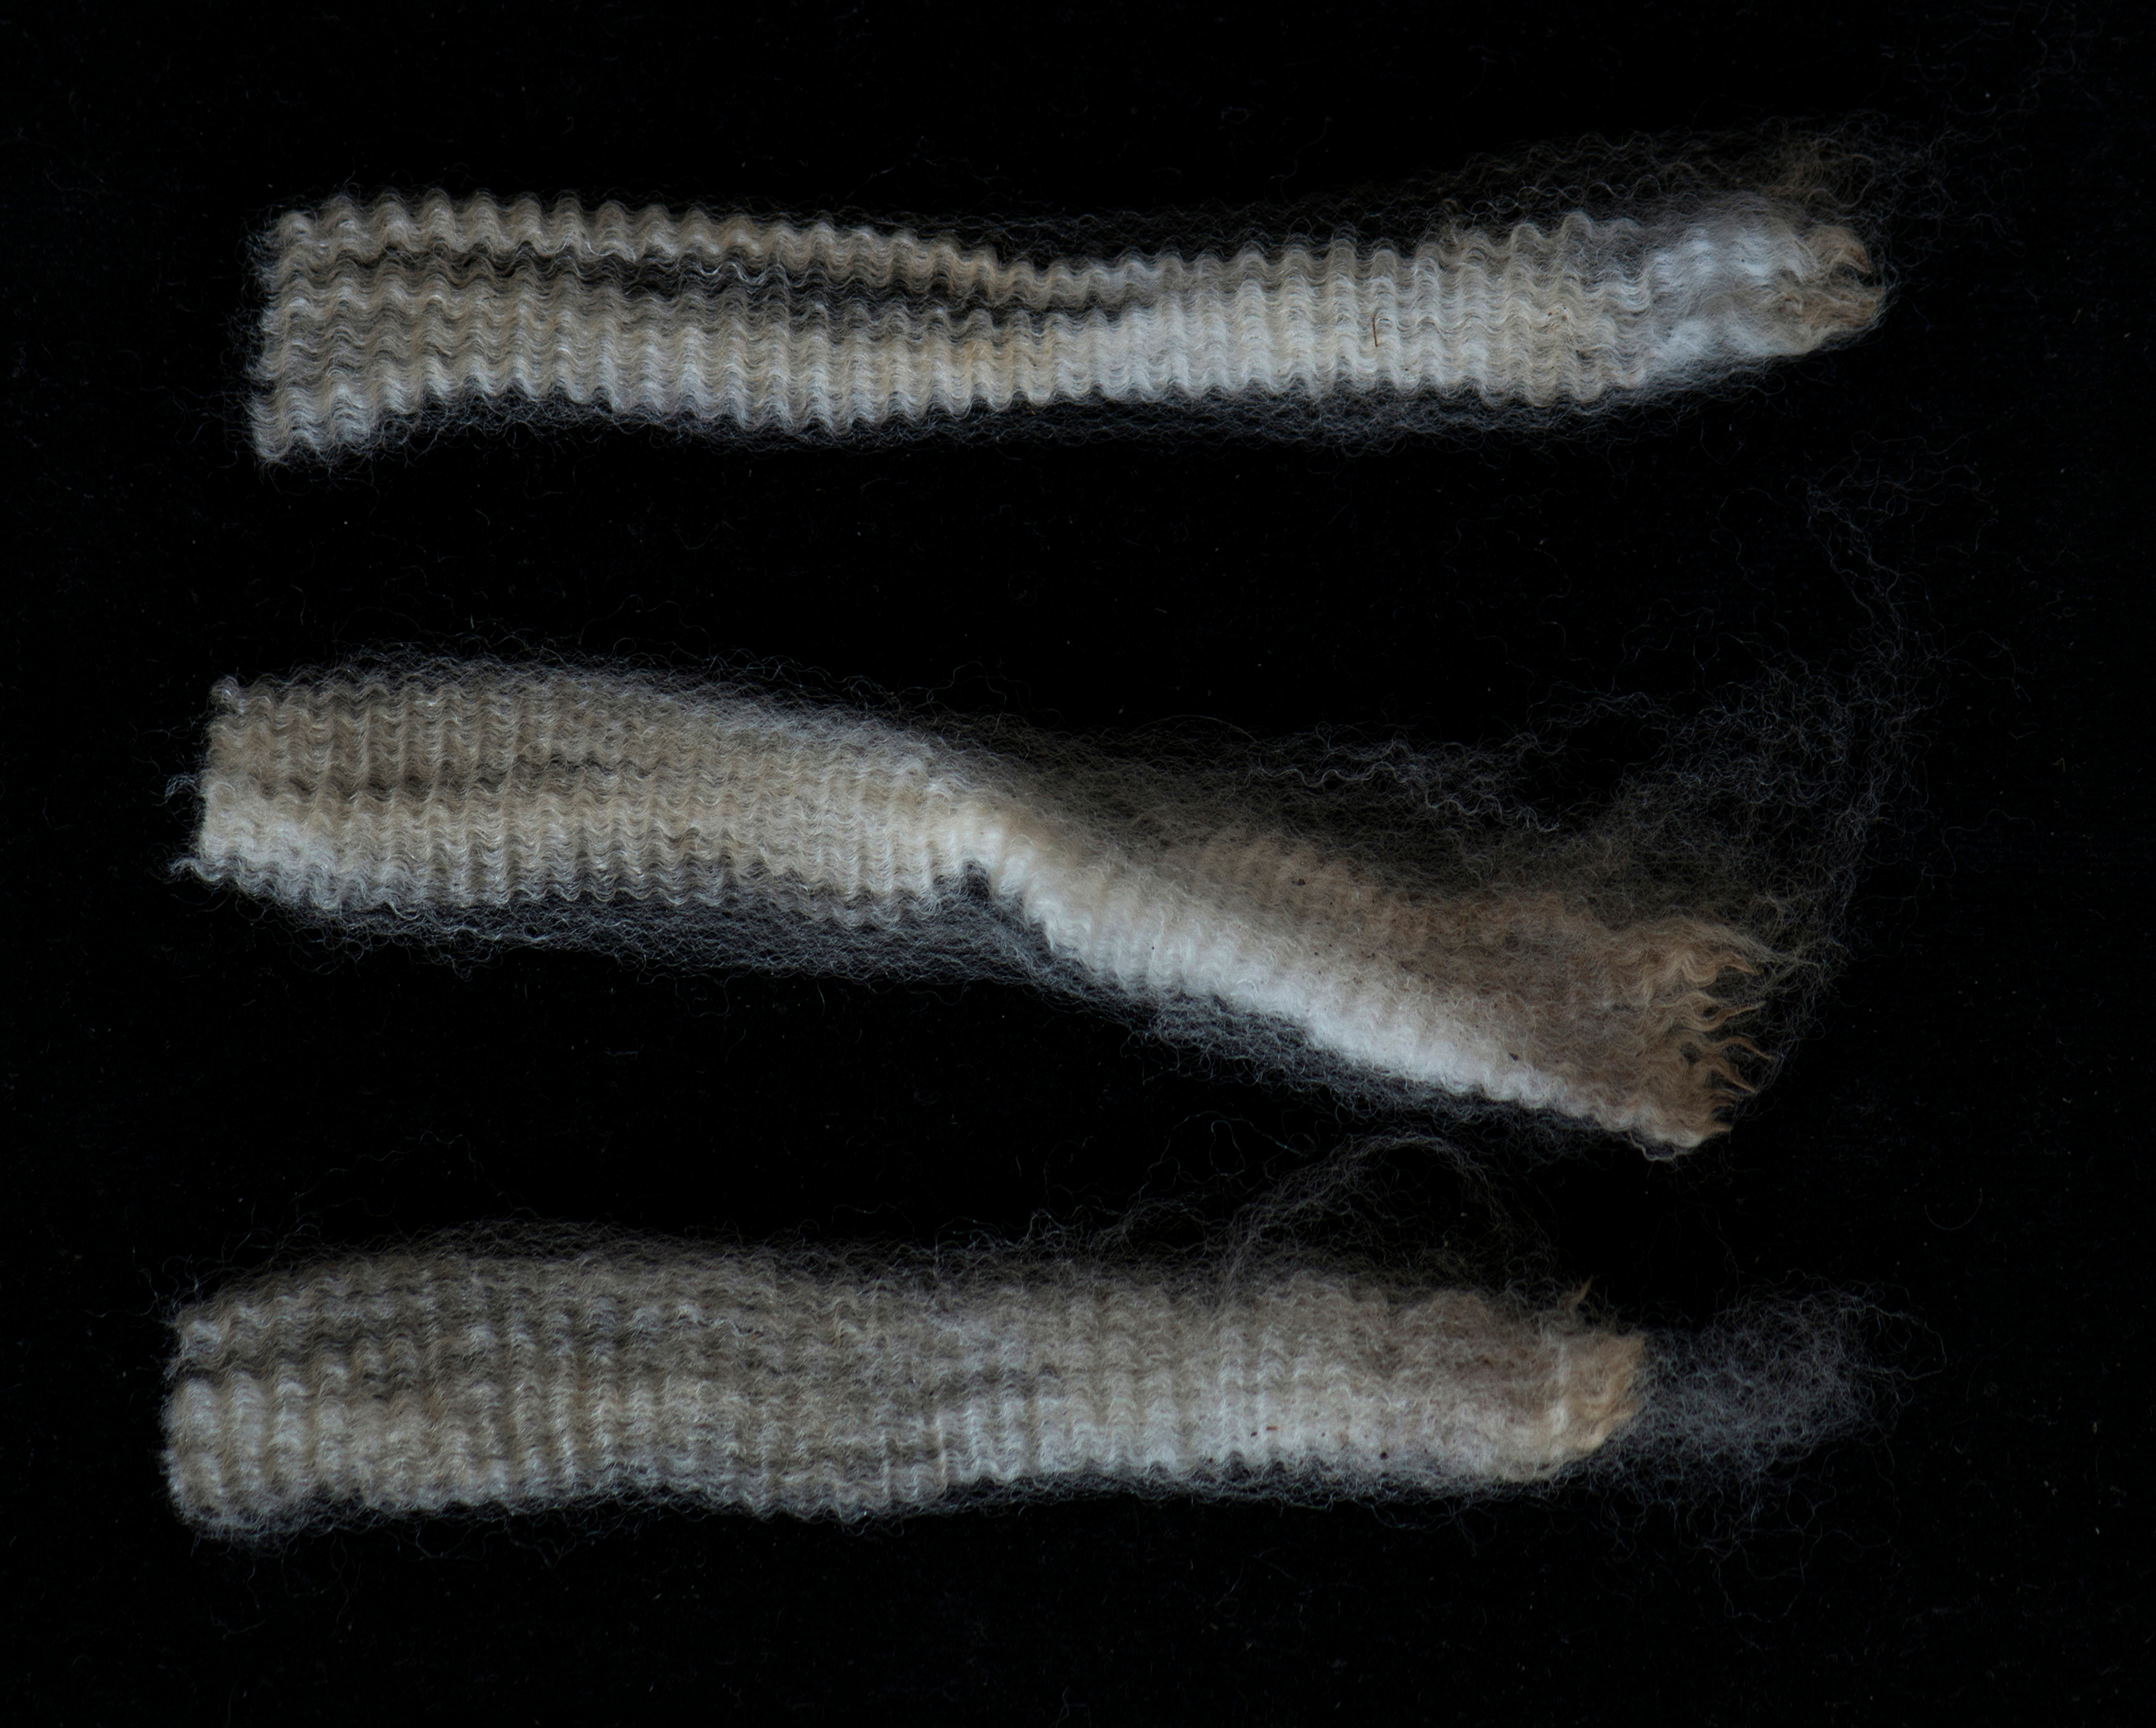
\includegraphics[width=1.0\textwidth,angle=180]{figwoolphoto.jpg}
  \includegraphics[scale=0.39]{figrule.jpg}
  \caption{Photograph of a ruler taken under the same conditions as Figure~\ref{fig:woolphoto}}
  \label{fig:ruler}
\end{figure}

%\end{document}



To determine the printed ( or screen) magnification of the Figure~\ref{fig:woolphoto} one measures a convenient length ( eg 10cm) on the ruler image in Figure~\ref{fig:ruler} and calculates the ratio of measured length to actual length, as above. For example when printed on an A4 page 10cm on the ruler image measures 8.5cm so the magnification of both the ruler image and Figure~\ref{fig:woolphoto} is 0.85.

\end{document}
